\chapter{Daten und Methodik}\label{daten-und-methodik}

\section{Korpus}\label{korpus}

\subsection{Auswahl der Zeitungen und des Untersuchungszeitraums}\label{auswahl-der-zeitungen-und-des-untersuchungszeitraums}

Für das dieser Arbeit zugrundeliegende Korpus wurden Artikel der Online-Ausgaben drei großer deutscher Zeitungen erhoben: \textsc{Spiegel} bzw. \textsc{Spiegel} \textsc{Online}, \textsc{Taz} bzw. \textsc{Taz} \textsc{Online} und \textsc{Welt} bzw. \textsc{Welt} \textsc{Online}. Obwohl alle genannten Zeitungen auch z.\,B. über das \emph{DeReKo} verfügbar sind, wurde entschieden, ein eigenes Korpus aufzubauen. Der Grund dafür ist, dass in großen Referenzkorpora aus urheberrechtlichen Gründen stets nur kleine Text-Ausschnitte zu Zeitungstexten ersichtlich sind. Zur explorativen Entwicklung einer Methode ist es jedoch notwendig, die vollen Texte zur Verfügung zu haben, sie nach eigenem Bedarf aufbereiten und in die einzelnen Verfahren einspeisen zu können.

Alle drei Online-Zeitungen stellen sogenannte ‚Leitmedien` \autocite{jarrenLeitmedienAlsQualitaetsmedien2011} dar. Für eine ausführliche Darstellung der Rolle, die die Analyse von Zeitungstexten aus Leitmedien in der Diskurslinguistik und für epistemologische Zugänge spielt, sei auf den rezenten und ausführlichen Überblick bei Drommler \autocite*{drommlerNationaleIdentitaetBerliner2024} verwiesen.\footnote{Der Autor bezieht sich dabei weitenteils auf gedruckte Zeitungen. Die Ausführungen sollten sich m.\,E. jedoch auf die Online-Ausgaben der Zeitungen übertragen lassen, zumal die Texte oft identisch sind.} Folgende Punkte möchte ich, ihm folgend, herausstellen:

\begin{enumerate}
\def\labelenumi{\arabic{enumi}.}
\item
  Zuvorderst ist der gegenstandskonstitutive Wert von Massenmedien hervorzuheben. Diese „schaffen oder strukturieren häufig überhaupt erst die interessierenden Diskurse/ Diskursphänomene, indem sie sie in der öffentlichen Arena erscheinen lassen`` \autocite[231]{drommlerNationaleIdentitaetBerliner2024}.
\item
  So tragen sie nicht nur zur Konstitution, sondern auch zur Verbreitung von Wissenselementen bei und sind „in modernen Gesellschaften nach wie vor von entscheidender Bedeutung, wenn es um die Distribution kollektiv geteilter Wissensbestände (in Prozessen der Meinungsbildung und -beeinflussung) geht, wenngleich mit abnehmender Tendenz`` \autocite[234]{drommlerNationaleIdentitaetBerliner2024}.
\item
  Sie sind des Weiteren von Bedeutung für gesellschaftliche Meinungsbildungsprozesse \autocite[236]{drommlerNationaleIdentitaetBerliner2024}, auch aufgrund ihrer „Resonanz {[}\ldots{]} innerhalb des Systems der Massenmedien sowie als Elitenmedium`` \autocite[237]{drommlerNationaleIdentitaetBerliner2024}.
\end{enumerate}

Ihre Rolle in diskurssemantischen Untersuchungen verdichtet Drommler des Weiteren in der Metapher von „Medien als Steinbruch sprachlichen Materials`` \autocite*[232]{drommlerNationaleIdentitaetBerliner2024}, die er einer akteursfokussierten Medienanalyse entgegenstellt:

\begin{quote}
Ich bevorzuge die Steinbruch-Metapher, weil sie es einerseits gestattet, zu fragen, weshalb eine diskursive Formation so beschaffen ist, wie sie zutage liegt, und somit zumindest Raum lässt, falls auf den Medienakteur bezogene Aspekte für eine Befundinterpretation relevant werden sollten {[}\ldots{]}. Andererseits (und im Gegensatz zur Fundus-Metapher) suggeriert sie nicht, dass das Untersuchungsmaterial lediglich entnommen werden müsste. Die Gewinnung des Materials ist ein eigenständiger Arbeitsgang mit eigenen Begründungspflichten, eigenen Werkzeugen, eigenen Handgriffen und eigenen Entscheidungen, die langfristige Folgen für alle weiteren Bearbeitungsschritte bergen. \autocite[232]{drommlerNationaleIdentitaetBerliner2024}
\end{quote}

Die getroffene Auswahl der Leitmedien soll das politische Meinungsspektrum innerhalb der Gruppe der Leitmedien abdecken, wobei der \textsc{Taz} gemeinhin eine eher linksalternative Position zugeschrieben wird, die der oft als eher rechtsliberal wahrgenommenen Position der \textsc{Welt} entgegensteht. Der \textsc{Spiegel} hingegen gilt als Medium der linken Mitte. Diese auf \textit{common sense} basierende Einschätzung wird auch durch eine aktuelle quantitativ-inhaltsanalytische Studie \autocite{maurerFehltWasPerspektivenvielfalt2024} gestützt.\footnote{Untersucht wurde die Berichterstattung 47 deutscher Medien im Zeitraum April bis Juni 2023 \autocite[4]{maurerFehltWasPerspektivenvielfalt2024}.} Diese zeigt zum einen, dass die \textsc{Taz} unter den genannten Zeitungen diejenige ist, die Parteien links der Mitte am positivsten und Parteien rechts der Mitte am negativsten bewertet.\textsuperscript{.}\footnote{Es geht hier jedoch nur um relativ-positive Bewertungen -- insgesamt ist die Bewertung „deutlich überwiegend negativ {[}\ldots{]}: Fast alle 47 von uns untersuchten Medien haben sowohl Parteien links der Mitte als auch Parteien rechts der Mitte im Schnitt überwiegend negativ bewertet``.} Im Gegensatz dazu bewertet die \textsc{Welt} linke Parteien negativer und rechte Parteien positiver, während der \textsc{Spiegel} jeweils zwischen den Polen positioniert ist. Diese Verteilung spiegelt sich auch in der grundsätzlichen ideologischen Ausrichtung der jeweiligen Zeitungen wider (siehe \figref{fig:medien-ideologie-verortung}). Die \textsc{Taz} vertritt deutlich liberal-progressive und sozialstaatsorientierte Positionen, während die \textsc{Welt} eher zu konservativ-autoritären und marktliberalen Haltungen tendiert. Der \textsc{Spiegel} ist erneut auf beiden Achsen zwischen den Zeitungen zu verorten, tendiert aber -- wie die große Mehrheit der betrachteten Medien -- jeweils zum linken Spektrum.

\begin{figure}[t]
  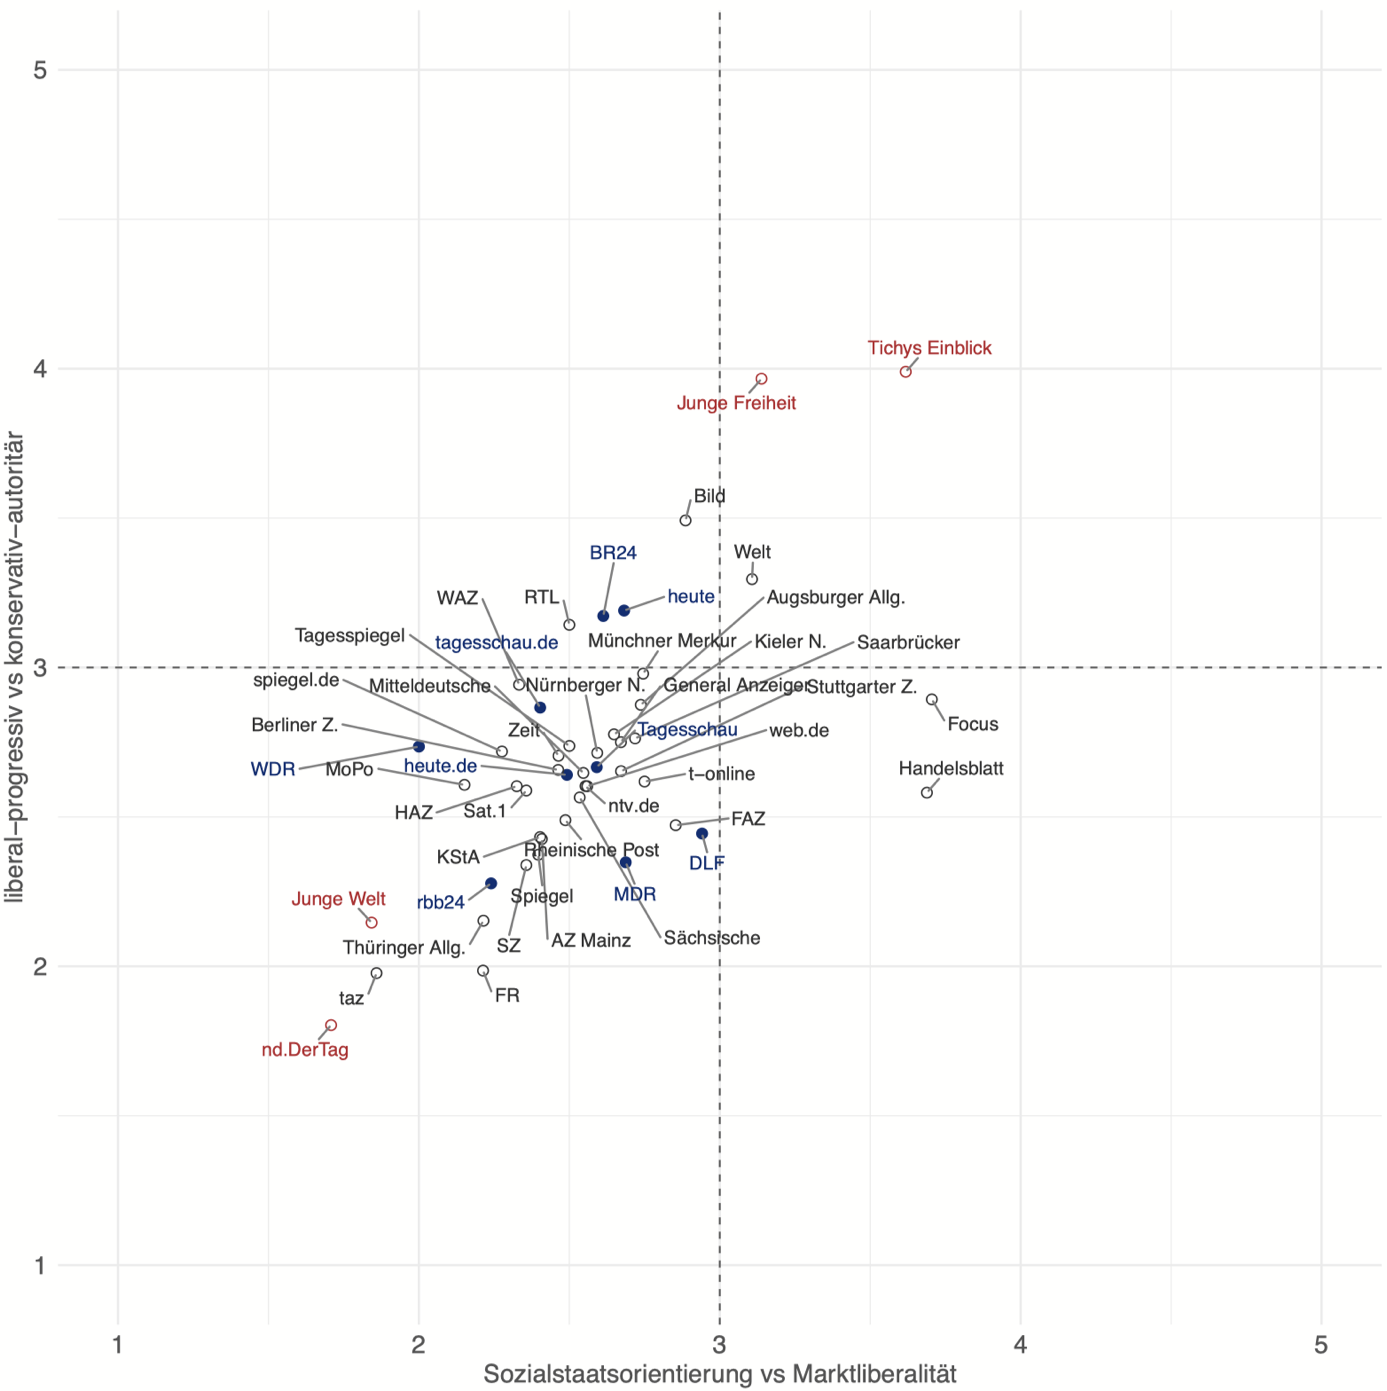
\includegraphics[width=\textwidth]{figures/media/image10.png}
  \caption{\label{fig:medien-ideologie-verortung}Verortung großer deutscher Medien in Hinblick auf ihre „ideologische Grundpositionierung`` (Abbildung 9 aus \citealt[17]{maurerFehltWasPerspektivenvielfalt2024}).}
\end{figure}

Dadurch, dass keine Boulevardmedien wie etwa die \textsc{Bild} oder Online-Medien des rechten Randes wie \textsc{Pi-News} oder \textsc{Compact} in das Korpus aufgenommen wurden, ist zu erwarten, dass die analytische Kontrastierung eher subtile Unterschiede im Framing von Extremismusvarianten zu Tage fördert denn grundlegend verschiedene Konzeptualisierungen. Es wurden also gewissermaßen Steinbrüche für die Erprobung des neu zu entwickelnden Werkzeugs ausgewählt, von denen eine gewisse Gleichartigkeit zu erwarten ist. Die ist auch insofern von Bedeutung, als die diachron geschichteten Subkorpora nicht nach Zeitungen getrennt untersucht werden und insofern eine gewisse Homogenität erfordern. Durch die ebenfalls erfolgende medienkonstrastive Analyse kann im Zeitungsvergleich divergierendes Framing im Anschluss genauer unter die Lupe genommen werden.

Letztlich ist auch zu reflektieren, dass sich mit der Entscheidung für Zeitungstexte auch eine Fortschreibung des „›written language bias‹ (vgl. Linell {[}1982{]} 2005), der in diskurslinguistischen Untersuchungen kritisch reflektiert werden sollte`` \autocite[39]{spitzmullerDiskurslinguistikEinfuhrungTheorien2011}, ergibt. Dies ist nicht von der Hand zu weisen und es wäre wünschenswert, mehr gesprochensprachliche Daten in Untersuchungen einzubeziehen; in der vorliegenden Untersuchung etwa journalistische Funk- und Fernsehbeiträge. Dem stehen jedoch forschungspraktische Gründe entgegen, da automatische Transkriptionsverfahren, die für den Aufbau eines Korpus in repräsentativer Größe notwendig sind, noch keine ausreichend guten Ergebnisse liefern. Es ist des Weiteren sinnvoll, im Rahmen der Entwicklung einer neuen korpuslinguistischen Methode auf vergleichsweise niedrigschwellig zu erlangende und zu prozessierende Daten zurückzugreifen, um sich nicht zu viele Herausforderungen zugleich ‚einzukaufen`.

\subsection{Verwendete Korpus-Software}\label{verwendete-korpus-software}

Die bei der Korpusaufbereitung und -Analyse eingesetzte Software musste in der Lage sein, ein sehr großes Korpus von über einer Milliarde Token verarbeiten zu können. Aus diesem Grund konnte auf verbreitete Tools wie die bezahl- bzw. lizenzpflichtige \emph{Sketch Engine} \autocite{kilgarriffSketchEngineTen2014} oder \emph{\#LancsBox} \autocite{brezinaLancsBoxV5x2020}, das nur vergleichsweise kleine Korpora von unter 10 Millionen Token noch effizient verarbeiten kann,\footnote{Siehe die FAQ unter \url{http://corpora.lancs.ac.uk/lancsbox/docs/pdf/FAQ.pdf}, S. 5. {[}18.12.2025{]}. Die neue Version \emph{\#LancsBox X} \autocite{brezinaLancsBox2023} ist auch in der Lage, größere Korpora zu händeln.} nicht zurückgegriffen werden. Es wurde daher entschieden, mit der \emph{Corpus Workbench} \autocite[CWB,][]{evertTwentyfirstCenturyCorpus2011} zu arbeiten, die in der Lage ist, große Korpora zu prozessieren und auf unterschiedlichen Annotationsebenen durchsuchbar bzw. analysierbar zu machen. Auch Kollokationsanalysen können flexibel auf unterschiedlichen Annotationen durchgeführt werden, was nicht in jedem Korpus-Tool möglich ist, in der hier entwickelten Methode jedoch genutzt wurde. Die Aufbereitung des Korpus folgte in Hinblick auf den Import in die CWB weitenteils Bubenhofers Einführung in die Korpuslinguistik \autocite*{bubenhoferEinfuhrungKorpuslinguistikPraktische2006}; weitere Schritte der Datenaufbereitung werden ausführlicher in den Kapiteln \ref{kenndaten-zum-korpus-und-korpusaufbereitung} und \ref{technisch-methodische-umsetzung-vom-rohen-text-zum-graphen} dargestellt.

Zur flexiblen Durchsuchung der CWB wurde mit dem \emph{R}-Package \emph{polmineR} \autocite{blaettePolmineRVerbsNouns2020} gearbeitet, das es ermöglicht, in der Programmiersprache \emph{R} mit der CWB zu kommunizieren. Es können so Abfragen gemacht werden, deren Ergebnisse unmittelbar im Anschluss in Visualisierungen überführt oder weiteren korpuslinguistischen Analysen unterzogen werden können. Es wurden mithilfe von \emph{polmineR} bzw. der CWB die Kollokations- und Keyword-Analysen sowie einzelne Konkordanz-Suchen durchgeführt.

Die Berechnung, das Clustering und die Exploration von Word Embeddings wurde in der Programmiersprache \emph{Python} und mithilfe des \emph{Word2Vec}-Moduls der \emph{Gensim}-Bibliothek \autocite{rehurekSoftwareFrameworkTopic2010} bzw. dessen Erweiterung \emph{Temporal Word Embeddings with a Compass} \autocite[TWEC,][]{dicarloTrainingTemporalWord2019} vorgenommen. Die Aufbereitung der Kollokations- und Word-Embedding-Daten als Netzwerkgraph geschah mit \emph{visNetwork}\footnote{\url{https://github.com/datastorm-open/visNetwork} {[}18.12.2025{]}}, der \emph{R}-Implementation des \emph{vis-network} Moduls der \emph{vis.js}-Bibliothek\footnote{\url{https://github.com/visjs/vis-network} {[}18.12.2025{]}}.

\subsection{Kenndaten zum Korpus und Korpusaufbereitung}\label{kenndaten-zum-korpus-und-korpusaufbereitung}
\largerpage
Im Rahmen der Datenerhebung wurden alle online ohne Zugangsbeschränkung verfügbaren Artikel der Online-Portale der Zeitungen bis einschließlich August 2021 gesammelt. Insgesamt wurden so 5\,207\,231 Texte bzw. rund 2 Mrd. Token erhoben, die sich in ungleichen Anteilen auf die drei Zeitungen verteilen (19,37 \% \textsc{Taz}, 18,40 \% \textsc{Spiegel}, 62,22 \% \textsc{Welt}). An Metadaten wurden neben publizierender Zeitung und Publikationsdatum auch Ressort, Autor*in, redaktionell vergebene Keywords und die URL erhoben. Im weiteren Verfahren werden davon jedoch nur das Publikationsdatum sowie die veröffentlichende Zeitung genutzt. In einem ersten Versuch konnte das Korpus aufgrund seiner Größe nicht in die CWB eingepflegt werden. Es wurde daher entschieden, ein Sampling der übermäßig repräsentierten \textsc{Welt}-Texte vorzunehmen und diese auf den Umfang der anderen Zeitungen zu reduzieren. Zu diesem Zweck wurden, diachron gleichmäßig verteilt, ca. 35 Prozent der \textsc{Welt}-Texte pro Monat zufällig aus dem Korpus entfernt, sodass das Korpus insgesamt (nicht jedoch in jedem Zeitabschnitt) medial ausgewogen ist (siehe~\figref{fig:subkorpora-umfang}). Es ergibt sich so ein 1\,282\,346\,988 Token umfassendes Korpus\footnote{Dieser und die nachfolgend genannten Token-Werte wurden in \emph{polmineR} mit der Funktion \emph{size()} ermittelt.}, das in acht diachrone sowie drei zeitungsspezifische Subkorpora untergliedert wurde.

Marchi geht ausführlich auf Fragen der diachronen Korpusgliederung ein und unterscheidet drei Varianten:

\begin{quote}
We can consider three ways to determine the level of aggregation of consecutive time periods in order to identify time units:

1 Text-lifecycle segmentation: based on the periodicity characterising the text type (e.g. a daily edition for a newspaper).

2 Top-down segmentation: based on standardised spans (typically a calendar year), or on contextual historical knowledge (e.g. a timeline of events), which is used to inform the segmentation (see for example Bartley \& Hidalgo-Tenorio 2016).

3 Bottom-up segmentation: based on internal variability, i.e. using distributional information to identify milestones in time, which can in turn be used to divide the corpus in subsets of data to compare against one another (Gries 2011).

I would like to argue that no one of these solutions is intrinsically optimal, but that the value of appropriateness always depends on the research questions. \autocite[179-180]{marchiDividingDataEpistemological2018}
\end{quote}

Die zeitliche Einteilung in dieser Arbeit entspricht Variante 2 und die diachronen Subkorpora umfassen jeweils drei Jahre. Eine Ausnahme ist das Subkorpus 2020--2021, das nur Daten bis einschließlich August 2021 umfasst. Dabei wurden also keine diskursspezifisch-inhaltlichen Kriterien wie einschneidende Gewaltereignisse bei Czulo et al. \autocite*{czuloEinflussExtremistischerGewaltereignisse2020} herangezogen, sondern kalendarische Einheiten. Diese sind in Bezug auf den Inhalt agnostisch und insofern zur datengeleiteten Ermittlung des Framings von Extremismus geeigneter, bei dem gewisse Ereignisse bzw. Handlungen extremistischer Akteure ja erst im Rahmen der Analyse aufgedeckt werden sollen. Möglichkeiten einer \emph{bottom-up segmentation} mithilfe strukturentdeckender Verfahren zu prüfen, wäre ein interessantes Desiderat, konnte aber im Rahmen dieser Arbeit nicht realisiert werden.

Der Umfang der Subkorpora wird in~\figref{fig:subkorpora-umfang} dargestellt; Tabelle 1 im Anhang umfasst die genauen Werte sowie die anteilige Verteilung der Zeitungen auf die diachronen Teilkorpora und \emph{vice versa}.

\begin{figure}
  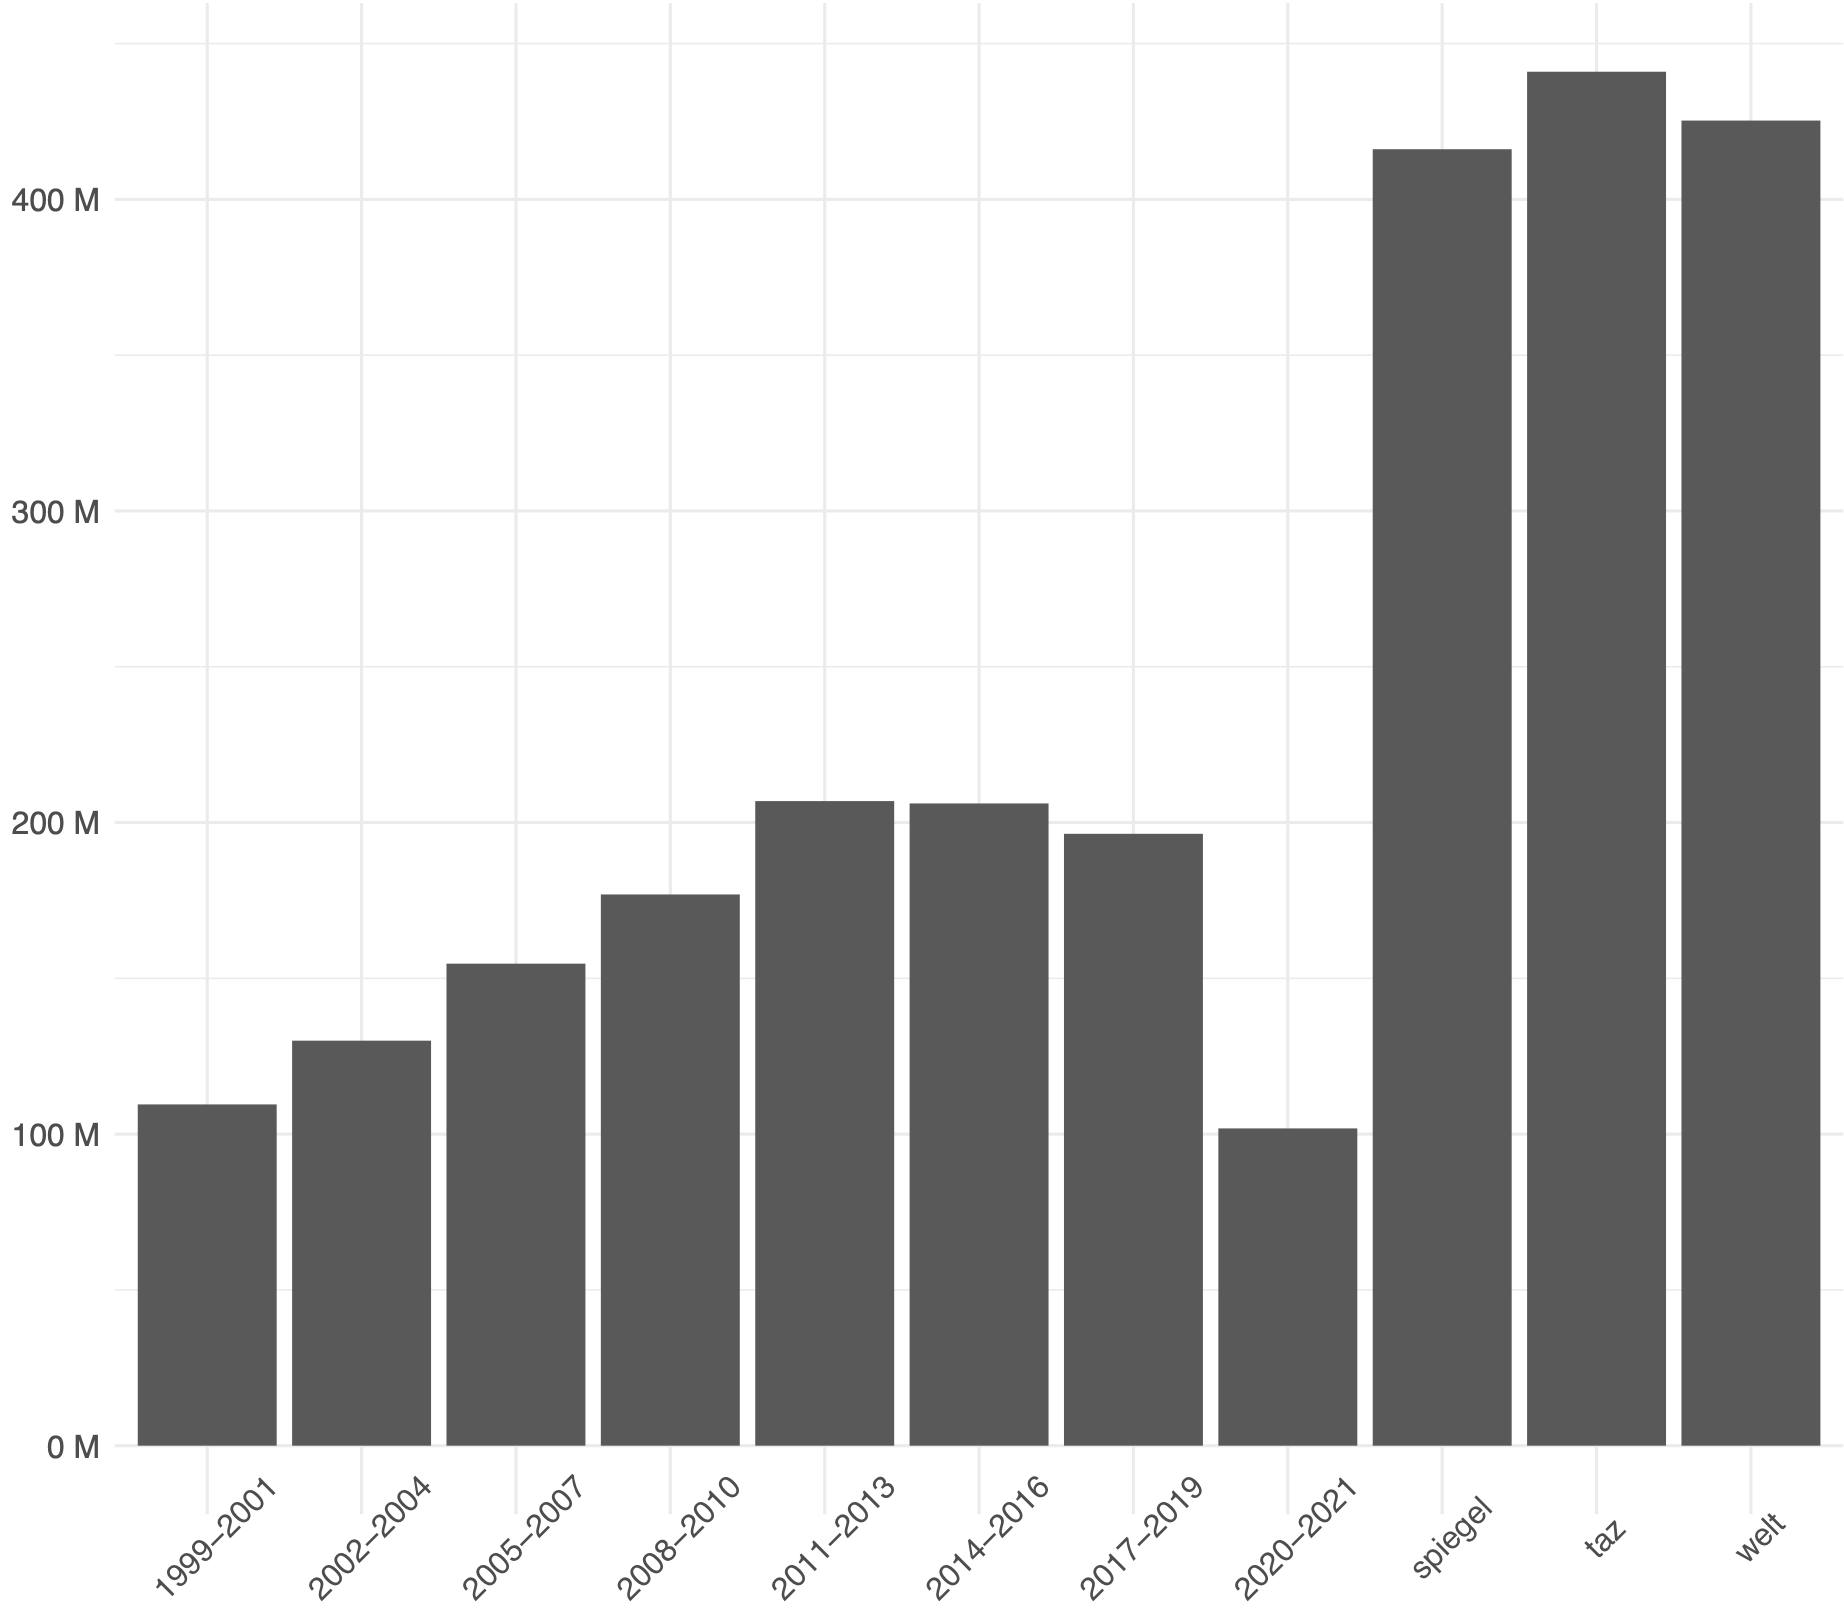
\includegraphics[width=\textwidth]{figures/media/image11.png}
  \caption{\label{fig:subkorpora-umfang}Umfang der Subkorpora in Millionen Token.}
\end{figure}


Die hier zugrundeliegende Tokenisierung wurde mit dem \emph{TreeTagger} \autocite{schmidProbabilisticPartSpeechTagging1994} vorgenommen, der zugleich ein POS-Tagging sowie eine Lemmatisierung des Korpus durchführte. Letztere Annotationen wurden im weiteren Verlauf jedoch kaum genutzt; einerseits um mögliche Fehlerquellen zu vermeiden, andererseits um das Bedeutungspotenzial der sprachlichen Oberfläche auszuschöpfen. Dass einzelne Wortformen einen deutlichen semantischen Mehrwert im Vergleich zur Arbeit mit Lemmata bieten, haben bereits Sinclair und Tognini-Bonelli herausgestellt (siehe \chapref{der-corpus-driven-ansatz}). Und auch Bubenhofer \autocite*[124-129]{bubenhoferSprachgebrauchsmusterKorpuslinguistikAls2009} weist auf das paradoxe Verhältnis hin, dass die Nutzung zusätzlicher Annotationen (auch) einen „Informationsverlust`` bedeutet. So zeigt sich auch im vorliegenden Korpus, dass z.\,B. im Zeitraum 2011--2013 das (ein Wort umfassende) Cluster \cluster{11\_Personen} eng mit dem thematischen Bereich ‚Straftaten \& Juristisches` assoziiert ist (u.\,a. \cluster{11\_Verdächtigen{\breakbar}Tatverdächtigen{\breakbar}mutmaßlichen\_Täter}, \cluster{11\_beschuldigt{\breakbar}verdächtigt{\breakbar}angeklagt}, \cluster{11\_Durchsuchungen{\breakbar}Razzia{\breakbar}Razzien}), während \cluster{11\_Person} im Singular ein deutlich anderes Kollokationsprofil aufweist und mit Clustern wie \cluster{11\_Verhalten}, \cluster{11\_Papst\_Franziskus{\breakbar}Franziskus{\breakbar}Vatikan}, \cluster{11\_Fragen} und \cluster{11\_Identität{\breakbar}Herkunft} vorkommt. Ein weiterer essenzieller Schritt bei der Korpusaufbereitung bestand darin -- Bubenhofer \autocite*{bubenhoferExplorationSemantischerRaeume2022} folgend --, signifikante, unmittelbar aufeinander folgende Wortverbindungen zu identifizieren und zu je einem Token zusammenzuführen. Dazu wurde die \emph{Phrases}-Funktion der \emph{Gensim}-\emph{Python}-Bibliothek eingesetzt (siehe auch \chapref{details-der-korpusaufbereitung}). Es wurden so zunächst signifikante Bi-Gramme identifiziert und -- markiert durch einen Unterstrich -- in das Korpus übernommen (z.\,B. \emph{Angela\_Merkel}). Der Vorgang wurde daraufhin wiederholt, um auch signifikante Tri-Gramme zu identifizieren. In seltenen Fällen, nämlich wenn zwei Bi-Gramme signifikant häufig aufeinander folgen, ergaben sich so auch 4-Gramme wie \emph{mutmaßlich\_rassistisch\_motivierten\_Anschlag}. Dieser Aufbereitungsschritt bildet nicht nur ab, dass sich Bedeutungseinheiten keinesfalls entlang von (orthographischen) Wortgrenzen ziehen lassen und approximiert so \emph{extended units of meaning} im Sinne Sinclairs \autocite*{sinclairUnitsMeaning1996}. Er leistet auch für Type-basierte Verfahren wie Kollokationen und Word Embeddings einen wichtigen Beitrag zur Disambiguierung. So wäre es in Bezug auf die Jugendorganisation der AfD wenig sinnvoll, Kollokationen oder benachbarte Embeddings zu \emph{Junge} oder \emph{Alternative} zu betrachten, da diese über alle Vorkommen der Ausdrücke berechnet werden. \tabref{tab:phrasing} zeigt die jeweiligen paradigmatischen Nachbarn der Ausdrücke und macht den Vorteil des Phrasings deutlich.\footnote{Die Tokenanzahl in den so prozessierten Korpora liegt etwa 20 \% unter den oben berichteten Werten, die genauen Werte finden sich in Tabelle 2 im Anhang.} Letztlich ist dieser Schritt auch unter Frame-semantischer Perspektive vorteilhaft, da auch \emph{FrameNet} Mehrworteinheiten als LE berücksichtigt \autocite[10]{ruppenhoferFrameNetIIExtended2016}.


\begin{table}
  \caption{Nächste Nachbarn im Word-Embedding-Modell 2020--2021 zu \emph{Junge}, \emph{Alternative} und \emph{Junge\_Alternative} mit Cosinus-Ähnlichkeit.}
  \label{tab:phrasing}
   \begin{tabularx}{\textwidth}{llX}
    \lsptoprule
              \emph{Junge}                    & \emph{Alternative}             & \emph{Junge\_Alternative} \\ % Header row
    \midrule
    \emph{junger\_Mann} (0.71)      & \emph{Ergänzung} (0.67)        & \emph{jA} (0.88)          \\
    \emph{Mann} (0.66)              & \emph{Alternativen} (0.66)     & \emph{Verfassungsschutz\_stuft} (0.80) \\
    \emph{Hund} (0.66)              & \emph{Option} (0.65)           & \emph{AfD-Flügel} (0.77)  \\
    \emph{Kleinkind} (0.65)         & \emph{echte\_Alternative} (0.62) & \emph{Nachwuchsorganisation} (0.75) \\
    \emph{Bub} (0.65)               & \emph{bessere\_Alternative} (0.56) & \emph{Beobachtungsfall} (0.73) \\
    \emph{elfjährige} (0.64)        & \emph{Lösung} (0.55)           & \emph{Gesamtpartei} (0.72) \\
    \emph{Säugling} (0.64)          & \emph{Blaupause} (0.54)        & \emph{rechtsextrem} (0.71) \\
    \emph{Teenager} (0.64)          & \emph{sinnvolle\_Ergänzung} (0.52) & \emph{rechtsextremen\_Verdachtsfall} (0.70) \\
    \emph{Baby} (0.63)              & \emph{Parallele} (0.52)        & \emph{Beobachtungsobjekt} (0.68) \\
    \emph{Senior} (0.63)            & \emph{Möglichkeit} (0.52)      & \emph{Identitäre\_Bewegung} (0.68) \\
    \lspbottomrule
   \end{tabularx}
  \end{table}

\tabref{tab:type_frequencies} weist die Type-Mengen pro Subkorpus aus und berichtet darüber hinaus, wie viele Types mindestens 25-mal im Korpus vorkommen und mithin bei der Berechnung der Word-Embedding-Modelle einbezogen wurden (siehe \chapref{berechnung-und-clustering-der-word-embedding-modelle}). Da durch die Mindestfrequenz ein großer Teil des \emph{long tail} der Zipfschen Häufigkeitsverteilung von Wörtern abgeschnitten wird, machen sie nur einen Bruchteil der gesamten Type-Menge aus.

\begin{table}
  \caption{Type-Anzahlen und Type-Anzahlen mit einer Mindestfrequenz von 25 pro Subkorpus.}
  \label{tab:type_frequencies}
   \begin{tabular}{lrr}
    \lsptoprule
    Subkorpus     & Types      & Types $\geq$ 25\\ %table header
    \midrule
    1999--2001  & 2541673  & 132041 \\
    2002--2004  & 2759025  & 148597 \\
    2005--2007  & 2994777  & 168204 \\
    2008--2010  & 3048237  & 183405 \\
    2011--2013  & 3196110  & 203417 \\
    2014--2016  & 3163474  & 201286 \\
    2017--2019  & 2910547  & 190915 \\
    2020--2021  & 1864503  & 110389 \\
    \textsc{Taz}  & 5789089  & 365815 \\
    \textsc{Spiegel} & 4883715  & 342740 \\
    \textsc{Welt} & 5002421  & 355619 \\
    \lspbottomrule
   \end{tabular}
  \end{table}

\section{Methodik und Operationalisierung}\label{methodik-und-operationalisierung}

\subsection{Prozess der Methodenentwicklung}\label{prozess-der-methodenentwicklung}

Dieses Kapitel soll einen kurzen Überblick über das Vorgehen bei der Entwicklung der Methode geben sowie ihre Funktionsweise in Kürze skizzieren. In den folgenden Abschnitten wird anschließend ausführlicher auf methodische Hintergründe, Operationalisierungen und die technische Realisierung eingegangen. Das Ansinnen war es, semantische Frames im Sinne Busses \autocite*{busseFrameSemantikKompendium2012} in einem datengeleiteten Zugriff kontextspezifisch zu rekonstruieren. Dabei sollte geprüft werden, inwiefern dies in einem quantitativen, datengeleiteten Zugriff möglich ist: Zum einen sollte die Bearbeitung großer und repräsentativer Korpora ermöglicht werden, zum anderen über einen distributionell-semantischen Zugriff die Bedeutung sprachlicher Einheiten erfasst und zu den ermittelten Frames bzw. Frame-Strukturen in Beziehung gesetzt werden. Die Hypothese ist dabei, dass (Frame\mbox{-})semantische Strukturen distributionellen Strukturen der sprachlichen Oberfläche entsprechen und dass beide in einem emergentistischen Zugang freigelegt werden können. Ein besonderes Potenzial der Nutzung quantitativer Verfahren liegt auch in der Ermöglichung einer probabilistischen Modellierung, die Frame-Relationen gegenstandsadäquat nicht absolut, sondern als graduelles Phänomen beschreiben kann.

Die Methode wurde in einem explorativen Prozess entwickelt, in dem mit unterschiedlichen korpuslinguistischen Verfahren experimentiert wurde, die sich in Diskursanalysen bewährt haben (siehe \chapref{distributionell-semantische-methodik}). Recht bald bewies sich das Potenzial von Word Embeddings, Wortsemantik zu erfassen und in einem quantitativen Zugang untersuchbar zu machen. Auch dass die paradigmatische Distribution der Wörter im Vektorraum als FE interpretierbar ist, wurde deutlich und durch eine Cluster-Analyse systematisch umgesetzt (siehe \chapref{geclusterte-word-embeddings-als-frame-elemente}). Frame-Relationen zwischen den FE wiederum konnten anschließend über das etablierte Verfahren der Kollokationsanalyse abgebildet werden. In \emph{corpus-driven} Manier wurden dabei die Kollokationen aller FE miteinander berechnet, was die Analyse und Visualisierung als rekursive Netzwerkstruktur, d.\,h. als Kollokationsnetzwerk, und mithin die Realisierung Frame-theoretischer Annahmen zur Organisation von Frames, ermöglichte (\chapref{kollokation-von-word-embedding-clustern-als-frame-relationen-und-perspektivierung-kollokationsnetzwerke-als-frames}--\ref{netzwerk-communities-als-thematische-teil-frames}). Nach weiteren methodischen Schritten der quantitativen Informationsanreicherung können die so korpus- bzw. kontextspezifisch ermittelten Frames dann interpretiert und kontrastiert werden. Leitlinien bei der Methodenentwicklung waren, dass die ermittelten diskursiven Frame-Strukturen sowohl in Hinblick auf Frame-semantische Annahmen als auch auf die kondensierten minimalen Anforderungen an einen Extremismus-Frame (\chapref{inhaltliche-mindestanforderungen-an-einen-extremismus-frame}) fruchtbar zu interpretieren sein mussten.

Die entwickelte Methode wurde unter dem Namen \emph{FDgrapher} (\emph{Frame and Discourse Grapher}) auf GitHub (\url{https://github.com/feldmueller/FDgrapher}) veröffentlicht.

\subsection{\texorpdfstring{Begriffsklärungen: Quantitativ und qualitativ -- \emph{corpus-driven} und \emph{corpus-based} sowie die Rolle von Hermeneutik}{Begriffsklärungen: Quantitativ und qualitativ -- corpus-driven und corpus-based sowie die Rolle von Hermeneutik}}\label{begriffsklaerungen-quantitativ-und-qualitativ-corpus-driven-und-corpus-based-sowie-die-rolle-von-hermeneutik}

\chapref{der-corpus-driven-ansatz} hat die grundlegenden Herangehensweisen von \emph{corpus-driven} und \emph{corpus-based} Ansätzen bereits skizziert. Im Folgenden sollen die Begriffe noch einmal präziser gefasst und in Hinblick auf konkrete Methoden sowie die Begriffe ‚quantitativ` und ‚qualitativ` (im Kontext korpuslinguistischer Arbeiten) verortet werden. Dies erscheint mir notwendig, da es seit der Prägung der Begriffe einerseits methodische Neuerungen, andererseits auch einen semantischen Wandel der Termini gegeben hat. Die Analyse einzelner Konkordanzen etwa, wie Tognini-Bonelli \autocite*{tognini-bonelliCorpusLinguisticsWork2001} sie zum zentralen Bestandteil ihrer Analysen macht, würdeheute wohl nicht mehr als \emph{corpus-driven} bezeichnet werden.

Die im Folgenden vorgenommene definitorische Unterteilung orientiert sich an Meißner et al. \autocite*{meissnerKorpusanalyse2016}, die korpuslinguistische Methoden einerseits in quantitative und qualitative, andererseits in korpus- und einheitenbezogene Verfahren unterteilen. Als ‚quantitative` Verfahren fasse ich mit Meißner et al. \autocite*[309]{meissnerKorpusanalyse2016} alle Korpusmethoden, die primär auf dem systematischen „Zählen von Einheiten`` beruhen und dabei sowohl Token bzw. Types als auch beliebige andere Korpusannotationen zur Grundlage der Zählung machen können. Im Gegensatz dazu begreife ich als ‚qualitativ` solche Methoden, die primär auf die Lektüre einzelner Belegstellen oder ganzer Texte zurückgreifen.

Zusätzliche Definitionselemente stellen m.\,E. eine unnötige Verengung der Begriffe dar. So heißt es bei Meißner et al. weiter zur quantitativen Methodik:

\begin{quote}
Ein Vorgehen im Sinne einer quantitativen Korpusanalyse bedeutet, den Untersuchungsgegenstand in suchbarer und auszählbarer Form zu operationalisieren und dabei theoretische Konzepte in empirische Häufigkeiten zu übersetzen. Die Fragestellung wird dabei so formuliert, dass die Häufigkeit, welche im Korpus unter den in Frage stehenden Bedingungen ermittelt wird, die abhängige Variable darstellt (vgl. Stefanowitsch 2005). \autocite[309]{meissnerKorpusanalyse2016}
\end{quote}

Dieses Vorgehen ist in der Praxis zwar in der Tat häufig anzutreffen und entspricht der klassischen quantitativen hypothesentestenden Methodik. Die Definition lässt jedoch \emph{corpus-driven} verfahrende Ansätze außer Acht, die gerade nicht mit vorausgesetzten theoretischen Konzepten und deren Operationalisierung arbeiten, sondern aus frequenzbasierten Daten theoretische Konzepte ableiten. Auch „das Ziel bestimmte in den Korpusdaten abgebildete (sprachliche) Phänomene zunächst zu ermitteln, sie zu klassifizieren, einzuordnen und zu interpretieren``, wie Meißner et al. \autocite*[312]{meissnerKorpusanalyse2016} im Anschluss an Scherer \autocite*{schererKorpuslinguistik2006} als Charakteristikum qualitativer Methoden ansetzen, gilt nur, wenn man quantitativ-datengeleitete Ansätze ignoriert, die ja ebenso verfahren. Letztlich ist gerade die Annahme, dass Interpretation bzw. ein „hermeneutisches Vorgehen`` \autocite[313]{meissnerKorpusanalyse2016} qualitative von quantitativen Ansätzen abgrenzt m.\,E. nicht sinnvoll, wenn auch weit verbreitet.\footnote{So etwa bei Busse \autocite*[202]{busse33LexikFrameanalytisch2017}, der eine „{[}q{]}uantitative oder qualitative (‚objektivistische` oder ‚hermeneutische`) Form der Analyse`` unterscheidet, bei Römer \& Wengeler \autocite*{roemerBackRootsVerteidigungsrede2022} oder aus quantitativer Perspektive bei Ziem \autocite*{ziem3WortschatzII2017}. Siehe aber kritisch z.\,B. Storjohann \& Schröter \autocite*[190-191]{storjohannPrasenzUndAbsenz2013}.} Digitale, quantitative Methoden stellen eine Möglichkeit dar, sprachliche Zeichen durch Transformationen auf neue Art lesbar zu machen \autocite{bubenhoferDigitaleKulturlinguistikDigitalitaet2022}. Sie werden dabei ihrem ursprünglichen Verwendungszusammenhang enthoben und somit -- wie Bubenhofer \autocite*{bubenhoferVisuelleLinguistikZur2020} herausarbeitet -- dekontextualisiert und desequenzialisiert, was zunächst einen Verlust an Informationen bedeutet. Zugleich werden sie jedoch zu anderen -- unter Umständen über das gesamte Korpus verteilten -- Zeichen in Bezug gesetzt und so rekontextualisiert. Eine Keyword-in-Context-Liste (KWiC-Liste) etwa ist

\begin{quote}
eine Anleitung zur Interpretation, die entweder jedem einzelnen Eintrag der Liste gerecht werden will oder aber eine Musterhaftigkeit in ihrem Ensemble sieht. Damit ist die Liste eben nicht nur einfach ein Verweisindex auf die ursprünglichen Kontexte, sondern bildet zusätzlich einen neuen Kontext. \autocite[195]{bubenhoferVisuelleLinguistikZur2020}
\end{quote}

Neben diesem -- gerade für die Diskurslinguistik zentralen -- Potenzial\footnote{Zentral für die Diskursanalyse ist dieses Potenzial besonders dann, wenn Diskursanalyse mit Spitzmüller \& Warnke \autocite*{spitzmullerDiskurslinguistikEinfuhrungTheorien2011} als ‚transtextuelle` Analyse begriffen wird oder mit Busse \autocite*[24]{busseDiskursSpracheGesellschaftliches2013} „als eine Form der Wort-, Satz- oder Textsemantik {[}\ldots{]}, die Beziehungen zwischen Wort- oder Satzbedeutungen und Texten auch dann analysiert, wenn die Bezugsgrößen aus verschiedenen Texten stammen sollten``.} liegt der Wert quantitativ-korpuslinguistischer Verfahren auch darin, Gütekrieterien wie Validität und Reliabilität gerecht zu werden \autocite{scharlothWuchernRhizomeLinguistische2013}. Dies bedeutet jedoch nicht, dass Analyseergebnisse ‚objektiv` wären oder für sich selbst sprechen könnten. Stattdessen müssen sie in einem Zugang, den man mit Schröter \autocite*[363-364]{schroeterWennMenschenAuseinandergehn2012} als ‚quantitative Hermeneutik`\footnote{Ihr Vorgehen ist allerdings primär qualitativ ausgerichtet und die quantitativen Analysen haben nur ergänzenden Charakter, sodass es sich durchaus um eine Neuausrichtung des Begriffs handeln würde.} bezeichnen könnte, gelesen werden. Dabei ist klar, dass der Zugang nicht voraussetzungsfrei ist. Gerade der häufig erhobene Einwand, dass ja das Korpus und seine Zusammenstellung durch die Forschungsperson einen gewichtigen Einfluss auf die Analyseergebnisse habe, trifft natürlich vollkommen zu. Er ist jedoch insofern auch etwas eigentümlich, als es in korpuspragmatischen Analysen ja geradezu darum geht, den Einfluss des Kontextes, den man im Korpusaufbau modellieren möchte, abzubilden; also gerade nicht „die Sprache`` abzubilden, sondern „auf der Basis verschiedener Datensätze unterschiedliche semantische Räume zu modellieren und miteinander zu vergleichen`` \autocite[218]{knuchelMachineLearningUnd2023}. Auch die Wahl der eingesetzten Algorithmen hat einen fundamentalen Einfluss auf die Analyseergebnisse. ‚Objektiv` -- oder vielleicht eher ‚unvoreingenommen` -- sind diese jedoch insofern, als sie „konsequent anti-intentionalistisch{[}{]}`` \autocite[724]{wilkSturmNieWar2021} sind. Sie fördern zwar, gesteuert durch die Forschungsperson, eine bestimmte Musterhaftigkeit zu Tage, etwa in Bezug auf Wortdistributionen. Über diskursive Inhalte wissen sie jedoch nichts. Wenn also durch die Wahl solcher inhaltlich agnostischer Algorithmen Wort-Cluster wie \cluster{14\_Fremdenfeindlichkeit{\breakbar}Intoleranz{\breakbar}Antisemitismus} emergent werden, ist das ein überdeutlicher Hinweis darauf, dass Charakteristika des (Rechts\mbox{-})Extremismus als solche diskursiv realisiert werden, eine Rolle im Framing von Extremismus spielen und für die Frame-Semantik als lexikalische Evokationsmuster einzubeziehen sind. Zusammenzufassen ist also, dass „quantitativ{[}e{]} Analysen {[}\ldots{]} nicht Antworten auf Fragestellungen {[}sind{]}, sondern neue Daten, die vor einem geistes- und sozialwissenschaftlichen Hintergrund genauso hermeneutisch gedeutet werden müssen wie einzelne Texte`` \autocite[25]{bubenhoferWennLinguistikKorpuslinguistik2018}.

Die hier vorgenommene und vergleichsweise einfache Unterteilung ermöglicht es, alle wichtigen korpuslinguistischen Methoden trennscharf zu verorten. Zu den ‚quantitativen` Verfahren zählen so die folgenden von Meißner et al. \autocite*{meissnerKorpusanalyse2016} zusammengetragenen Methoden: die Berechnung und Analyse von Wort- bzw. Frequenzlisten, Keywords, N-Grammen, Kennwerten wie der Type-Token-Ratio, die quantitative Konkordanzsuche\footnote{Bei quantitativen Konkordanzsuchen geht es, anders als in ihrem qualitativen Pendant, nicht um die Lektüre einzelner Belegstellen, sondern um die Ermittlung der Frequenz eines Suchmusters im Korpus.} sowie die Kollokations- und die Kollostruktionsanalyse \autocite{stefanowitschCollostructionsInvestigatingInteraction2003}. Zu ergänzen sind Methoden bzw. Sprachmodelle, die auf komplexen statistischen Verfahren bzw. dem Training neuronaler Netze beruhen wie etwa Word Embeddings, Topic Modelling, Transformer-Sprachmodelle wie BERT \autocite{devlinBERTPretrainingDeep2019} und auch Large Language Models (LLMs) der neuesten Generation wie ChatGPT \autocite{openaiGPT4TechnicalReport2023}. Zu den ‚qualitativen` Verfahren zähle ich lediglich die eingehende Lektüre von Konkordanzen oder ganzer Korpustexte.

Die Unterteilung in \emph{corpus-based} und \emph{corpus-driven} Verfahren weist Überlappungen mit der quantitativ-qualitativ-Abgrenzung auf, ist jedoch von dieser zu unterscheiden. So unterliegt zwar allen \emph{corpus-driven} Korpusmethoden zugleich eine quantitative Funktionsweise und zumindest die qualitative Lektüre einzelner Konkordanzen ist immer \emph{corpus-based}, jedoch können \emph{corpus-based} Methoden sowohl qualitativer als auch quantitativer Natur sein. Im Verständnis dieser Arbeit entspricht die Differenzierung in \emph{corpus-based} und \emph{corpus-driven} Ansätze grob der Unterteilung von Meißner et al. in korpus- und einheitenbezogene Verfahren. Als \emph{corpus-based} bzw. einheitenbezogen verstehe ich alle Methoden, die zu einem vorgegebenen Suchmuster Ergebnisse liefern. Darunter fällt prototypisch die Konkordanzsuche, die in einem qualitativen Zugang genutzt werden kann, um Kotexte des Suchmusters in der KWIC-Ansicht zu betrachten oder auch die „Quantitative Konkordanzsuche`` \autocite[311]{meissnerKorpusanalyse2016}, die nicht auf die Sichtung einzelner Belegstellen, sondern auf die Ermittlung der Frequenz des abgefragten Suchmusters zielt. Als weiteres wichtiges Verfahren fällt die klassische Kollokationsanalyse, die zu einem Suchmuster Kollokate ermittelt, in diese Kategorie. Bei \emph{corpus-driven} bzw. korpusbezogenen Methoden wird hingegen darauf verzichtet, Suchausdrücke zu formulieren. Stattdessen wird das gewählte Verfahren auf das gesamte Korpus und alle auf der anvisierten Korpusebene enthaltenen sprachlichen Einheiten angewandt. So wird etwa bei einer Keyword-Analyse nicht ein einzelnes Wort vorgegeben und daraufhin ermittelt, ob dieses im Korpus signifikant häufiger als in einem Referenzkorpus vorkommt. Stattdessen werden \emph{alle} im Korpus enthaltenen Wörter zu Tage gefördert, die überzufällig häufig im Vergleich zu einem Referenzkorpus vorkommen. Ebenfalls zu den etablierten \emph{corpus-driven} Methoden zählen Wortlisten, N-Gramme, Kennwerte wie die Type-Token-Ratio, Word Embeddings, Topic Modelling, aber auch die Berechnung ganzer Kollokationsnetze, bei denen für jede sprachliche Einheit ein Kollokationswert in Bezug auf jede andere sprachliche Einheit ermittelt wird (so auch im Rahmen dieser Arbeit realisiert). Word Embeddings wiederum können auch in \emph{corpus-based} Manier genutzt werden, wenn nur zu ausgesuchten Wörtern distributionelle Eigenschaften abgefragt werden.

Letztlich ist festzuhalten, dass mithilfe dieser Definitionen zwar eine trennscharfe Zuordnung von Methoden möglich ist, in der Forschungspraxis jedoch quantitative und qualitative Verfahren zumeist kombiniert werden. Insbesondere die qualitative Sichtung von Konkordanzen zu quantitativ ermittelten sprachlichen Einheiten kann ein wichtiger Analyseschritt sein, um quantitative Zusammenhänge zu verstehen und insbesondere detailbezogene Analyseergebnisse abzusichern. So stellt Baker fest:

\begin{quote}
we have to make sure that what we \emph{think} is being counted is actually what the computer is counting. A wise corpus linguist always checks concordance data before drawing conclusions. \autocite[44]{bakerAcceptableBiasUsing2012}
\end{quote}

Während dem ersten Teil des Zitats vollumfänglich zuzustimmen ist und ein gutes Verständnis der verwendeten Methoden und ihrer Aussagekraft immer notwendig ist, ist die umfängliche Sichtung von Textbelegen bei frequenten Mustern und großen Korpora kaum noch möglich. Sie ist aufgrund der (re)kontextualisierenden Eigenschaft korpuslinguistischer Analyseergebnisse aber auch gar nicht immer notwendig:

\begin{quote}
So stehen beispielsweise maschinell berechnete Mehrworteinheiten, die statistisch für bestimmte Akteure, Institutionen oder Zeitepochen typisch sind, im Vordergrund, die anschließend diskurslinguistisch gedeutet werden. Diese Menge an Mehrworteinheiten mit gemeinsamer Typik hinsichtlich eines bestimmten Aspektes sind eine rekontextualisierte Liste -- mit Sprengkraft. Denn -- so die Kritik -- wie sollen die einzelnen Mehrworteinheiten ohne Rückgriff auf die „ursprünglichen`` Kontexte in den „eigentlichen`` Texten korrekt gedeutet werden? Dieser Einwand wird dann zur Konstruktion einer Dichotomie zwischen quantitativen und qualitativen Methoden verwendet und im besten Fall gefordert, dass beides miteinander verbunden werden müsse (Spitzmüller{\slash}Warnke 2011, 39; Niehr 2015, 144). Die Frage ist also, ob die rekontextualisierte Liste ernst genommen wird oder nicht -- ob der Pakt mit dem Teufel eingegangen wird, wie es der Literaturwissenschaftler Franco Moretti ausgedrückt hat: „what we really need is a little pact with the devil: we know how to read texts, now let's learn how not to read them`` (Moretti 2000, 57). \autocites[195]{bubenhoferVisuelleLinguistikZur2020}[siehe auch][]{bubenhoferDreiThesenVisualisierungspraktiken2016}
\end{quote}

Es findet sich des Weiteren eine Reihe methodologischer Vorschläge zur Kombination eher quantitativ-\emph{corpus-driven} ausgerichteter Verfahren mit qualitativ-\emph{corpus-based} Ansätzen. So sprechen etwa Stulpe \& Lemke \autocite*{stulpeBlendedReading2016} von \emph{blended reading} als eine Kombination von \emph{close} und \emph{distant reading} \autocite{morettiConjecturesWorldLiterature2000}; Kalwa \autocite*{kalwaKonstitutionKonzeptenDiskursen2019} spricht von \emph{Zooming in}{\slash}\emph{out} und Bubenhofer \autocite*{bubenhoferQuantitativInformierteQualitative2013} schlägt eine „quantitativ informierte qualitive Diskursanalyse`` vor, bei der qualitativere Analysen auf der Folie quantitativer Ergebnisse vorgenommen werden. In dieser von Bubenhofer vorgeschlagenen Heuristik werden qualitative Untersuchungen vor dem Hintergrund quantitativer Daten vorgenommen. Die Idee ist, dass diskursive Veränderungen und Regelmäßigkeiten besonders gut bei Kenntnis der musterhaften „seriellen Verwendung -- oder gerade auch der seriellen Vermeidung`` \autocite*[130]{bubenhoferQuantitativInformierteQualitative2013} gefunden bzw. aufgezeigt werden können.

\subsection{Methoden der Distributionellen Semantik: Word Embeddings und Kollokationen}\label{methoden-der-distributionellen-semantik-word-embeddings-und-kollokationen}

\subsubsection{Kollokationen als syntagmatische distributionelle Muster}\label{kollokationen-als-syntagmatische-distributionelle-muster}

\subsubsubsection{Was sind Kollokationen?}\label{was-sind-kollokationen}

Die Berechnung von Kollokationen ist eine der wichtigsten Methoden der semantisch interessierten Korpuslinguistik. Begrifflich sind Kollokationen jedoch keinesfalls klar umrissen, Evert \autocite*[15]{evertStatisticsWordCooccurrences2005} spricht von „serious terminological confusion that surrounds the concept of collocations today``. Auf den Punkt bringt es Schmid \autocite*[235]{schmidCollocationHardPin2003}: Kollokationen sind „hard to pin down, but bloody useful``. Während der Begriff bei seinem Schöpfer John Rupert Firth \autocite*[194-195]{firthPapersLinguistics193419511957} noch eine eher vage Bedeutung hatte und das übliche (auch im Sinne des frequenten) gemeinsame Vorkommen von Wörtern bezeichnete (siehe auch \chapref{distributionelle-semantik}), haben sich im Laufe der Zeit in unterschiedlichen Forschungstraditionen verschiedene Definitionen etabliert. Zugrundegelegt werden dabei zum Teil eher frequenzbezogene, sprachstatistische Kriterien, zum Teil auch grammatische Dependenzbeziehungen oder Idiomatizität. Zur terminologischen Differenzierung wird mitunter der Begriff der ‚Kookkurrenz` herangezogen, der jedoch gleichermaßen heterogen verwendet wird. So sind für Bubenhofer Kollokationen durch ihr statistisch signifikant häufiges gemeinsames Auftreten in einem Korpus gekennzeichnet, wohingegen der Begriff der ‚Kookkurrenz` einfach gemeinsames Ko-Vorkommen meint:

\begin{quote}
Unter ‚Kollokationen` verstehe ich statistisch auffällige Kookkurrenzen. Das Plus von Kollokationen gegenüber Kookkurrenzen liegt also nur im statistischen Maß der überzufälligen Kombination. Kookkurrenzen beschreiben demnach in einem Syntagma aufeinander treffende Wörter, von denen nicht weiter bekannt ist, ob ihre Verbindung statistisch signifikant oder überhaupt besonders frequent ist. \autocite[122]{bubenhoferSprachgebrauchsmusterKorpuslinguistikAls2009}
\end{quote}

Auch bei Lemnitzer und Zinsmeister ist der Kollokationsbegriff ein Hyponym des Kookkurrenzbegriffes, sie setzen das Kriterium der statistischen Signifikanz allerdings bereits für Kookkurrenzen an und definieren Kollokationen sodann systemlinguistisch:

\begin{quote}
Eine Kollokation muss natürlich den oben genannten Kriterien {[}zur Kookkurrenz, T.F.{]} genügen, darüber hinaus aber auch eine innere Struktur, in Form einer Hierarchie zwischen Kollokationsbasis und Kollokator aufweisen. Darüber hinaus müssen die Glieder einer Kollokation in einer syntaktischen Beziehung zueinander stehen, z.\,B. als Kopf einer Verbalphrase und Kopf einer gleich- oder untergeordneten Nominalphrase, oder als Kopf einer Nominalphrase und Kopf einer untergeordneten Adjektivphrase. \autocite[179]{lemnitzerKorpuslinguistikEinfuhrung2015}
\end{quote}

Als Beispiele für so definierte Kollokationen geben sie etwa \emph{Zähne putzen}, \emph{Schlange stehen}, \emph{den Tisch decken} und \emph{dichtes Haar} an. Vor dem Hintergrund der vorliegenden umfangreichen (Überblicks\mbox{-})Literatur zu Kollokationen \autocites[siehe etwa][]{storjohannKookkurrenzAusKorpuslinguistischer2016, almela-sanchezLexicalCollocationAnalysis2018, bubenhoferSprachgebrauchsmusterKorpuslinguistikAls2009, evertStatisticsWordCooccurrences2005, stefanowitschCorpusLinguisticsGuide2020} sei an dieser Stelle darauf verzichtet, weitere Begriffsdefinitionen und -ansätze darzustellen. Definitorisch folge ich Bubenhofer und fasse Kollokationen als das überzufällig häufige Ko-Vorkommen von sprachlichen Einheiten auf, das korpuslinguistisch mithilfe unterschiedlicher Maße gemessen werden kann und so auch eine graduelle Auskunft über die Kollokationsstärke gibt. Dass dieser Ansatz „lumps together units that are linguistically quite different`` \autocite[231]{grangerFormulaicSequencesLearner2018}, also unterschiedliche Wortarten und neben Autosemantika auch Synsemantika zu Tage fördert, ist dabei in einer datengeleiteten Diskursanalyse nicht problematisch, sondern hat das Potenzial, auch unauffällige musterhafte Sprechweisen freizulegen.

\subsubsubsection{Wie funktioniert die Berechnung von Kollokationen?}\label{wie-funktioniert-die-berechnung-von-kollokationen}

Grundlage der Berechnung von Kollokationen sind drei wesentliche Parameter: die Suchanfrage, das Kollokationsfenster und das statistische Maß, das über Signifikanz und Rangfolge der Ergebnisse entscheidet. Mit der Suchanfrage wird das sprachliche Muster festgelegt, zu dem Kollokatoren im Korpus ermittelt werden sollen. In der Regel sind dies einzelne Wörter, d.\,h. Wortformen oder Lemmata. Es ist jedoch auch denkbar -- je nach Möglichkeiten der Korpussoftware -- auf beliebigen anderen Annotationsebenen zu suchen. So lässt sich z.\,B. abfragen, welche POS-Tags miteinander vorkommen oder -- wie in der folgenden Analyse -- welche Wort-Cluster Kollokationen bilden. Die Suchanfrage zu den Ergebnissen der Kollokationsanalyse in \tabref{tab:collocation_analysis}, die mit \emph{polmineR} im Teilkorpus 2020--2021 durchgeführt wurde, lautet etwa \emph{cooccurrences(``{[}word = `Hanau'{]}'', l = 5, r = 5, method = ``ll'', cqp = TRUE)}. Sie legt fest, dass Kollokationen zur Wortform \emph{Hanau} berechnet werden sollen, dass das Kollokationsfenster je fünf Wörter zur linken und rechten des Wortes umfassen soll, dass als statistisches Maß die \emph{Log-Likelihood} \autocite{dunningAccurateMethodsStatistics1993} verwendet werden soll sowie als Abfragesprache CQP \autocite{evertTwentyfirstCenturyCorpus2011}. \tabref{tab:collocation_analysis} listet die von \emph{polmineR} bzw. der unterliegenden CWB ausgegebenen Werte. \emph{Count\_coi} zeigt dabei an, dass z.\,B. \emph{Anschlag} 358 Mal im Umfeld von \emph{Hanau} auftaucht; \emph{count\_ref}, dass \emph{Anschlag} 3179 Mal ohne \emph{Hanau} auftritt. Bei einer zufälligen Verteilung der Wörter im Korpus wäre allerdings davon auszugehen, dass \emph{Anschlag} nur 1,42 Mal (\emph{exp\_coi}) mit \emph{Hanau} kookkurriert und 3535,58 Mal ohne \emph{Hanau} (\emph{exp\_ref}). Diese Diskrepanz bedingt sodann den errechneten \emph{Log-Likelihood}-Wert (\emph{ll}) von 3288,71.

\begin{table}
\caption{Beispiel-Output einer Kollokationsanalyse mit \emph{polmineR} zu \emph{Hanau} im Subkorpus 2020--2021.}
\small
\label{tab:collocation_analysis}
 \begin{tabular}{lrrrrr}
  \lsptoprule
  word & count\_coi & count\_ref & exp\_coi & exp\_ref & ll \\
  \midrule
  \emph{Anschlag}              & 358   & 3179    & 1.42   & 3535.58   & 3288.71 \\
  \emph{Halle}                 & 245   & 5235    & 2.20   & 5477.80   & 1837.30 \\
  \emph{in}                    & 1856  & 1749678 & 701.88 & 1750832.12 & 1344.40 \\
  \emph{Opfer}                 & 227   & 11983   & 4.89   & 12205.11  & 1303.45 \\
  \emph{von}                   & 1122  & 837359  & 336    & 838145    & 1153.76 \\
  \emph{rassistischen\_Anschlag} & 78  & 15      & 0.04   & 92.96     & 1138.29 \\
  \emph{nach}                  & 681   & 335175  & 134.59 & 335721.41 & 1125.60 \\
  \emph{neun}                  & 172   & 9137    & 3.73   & 9305.27   & 985.25 \\
  \emph{Hanau}                 & 100   & 3160    & 1.31   & 3258.69   & 673.52 \\
  \emph{Anschlags}             & 60    & 409     & 0.19   & 468.71    & 580.38 \\
  \lspbottomrule
 \end{tabular}
\end{table}

Das Kollokationsfenster als zweiter festzulegender Parameter bestimmt, wie viele Wörter zur Rechten und Linken der jeweiligen Treffer der Suchanfrage als potenzielle Kollokatoren berücksichtigt werden sollen. Einen Standardwert stellt hier ein Suchfenster von 5 Token zu beiden Seiten dar.

Das statistische Maß entscheidet letzten Endes darüber, ob die im Kollokationsfenster gezählten Token signifikante Kollokate des Suchmuster sind und wie stark die statistische Bindung zwischen ihnen ist. Würde man die Ergebnisse der \tabref{tab:collocation_analysis} zugrundeliegenden Analyse einfach nach der Frequenz des gemeinsamen Auftretens ordnen, würden die ersten fünf Ränge durch \emph{die}, \emph{der}, \emph{und}, \emph{in} und \emph{das} besetzt. Da diese Wörter jedoch generell häufig im Korpus vorkommen, ist es nicht weiter überraschend, dass sie auch gemeinsam mit \emph{Hanau} auftreten. Hier wird also das Prinzip der statistischen Signifikanz relevant, das mit einer gewissen Sicherheit ausschließen kann, dass die Types im Korpus einfach zufällig verteilt sind, sodass im Umkehrschluss von einer Kollokation auszugehen ist. Konventionell werden Signifikanzlevel verwendet, die mindestens eine Wahrscheinlichkeit von 5 \% (p \textless{} .05) versprechen, dass das Ergebnis „is not due to some sort of accidental sampling fluke, but rather reflects an actual difference in the language use of the two populations being examined`` \autocite[63]{bakerSociolinguisticsCorpusLinguistics2010}. Dieses Signifikanzlevel entspricht einem \emph{Log-Likelihood}-Wert von mindestens 3,84.

Verwendet man \emph{Pointwise Mutual Information} (PMI) statt \emph{Log-Likelihood} als statistisches Maß für die gleiche Analyse, ändert sich das Bild vollkommen und man erhält als Top-Kollokate \emph{mutmaßlich\_rassistisch\_motivierten\_Anschlag}, \emph{Wehrhafte\_Demokratie} und \emph{zentrale\_Trauerfeier}. Dies liegt daran, dass PMI seltenen, aber gegenseitig exklusiven Kollokationen einen deutlich höheren Stellenwert einräumt bzw. im Falle von \emph{Log-Likelihood} sogar eine Voraussetzung ist, dass Kollokate mindestens ein Mal außerhalb des Kollokationsfensters vorkommen.\footnote{Im Falle von \emph{Log-Likelihood} besteht eine Voraussetzung sogar darin, dass Kollokate mindestens ein Mal außerhalb des Kollokationsfensters vorkommen \autocite{blaetteComputeLoglikelihoodStatistics2020}.} D.\,h. immer, wenn im Korpus das 4-Gramm \emph{mutmaßlich\_rassistisch\_motivierten\_Anschlag} vorkommt, kommt auch \emph{Hanau} vor. Insgesamt ist die Kollokation mit nur 16 Vorkommen jedoch sehr selten im Vergleich zu denen in \tabref{tab:collocation_analysis} \autocites[siehe zu einem ausführlichen Überblick zu Kollokationsmaßen][]{evertStatisticsWordCooccurrences2005, evert58CorporaCollocations2009}.

\subsubsection{Word Embeddings als paradigmatische distributionelle Muster}\label{word-embeddings-als-paradigmatische-distributionelle-muster}

\subsubsubsection{Was sind Word Embeddings?}\label{was-sind-word-embeddings}

Embeddings bezeichnen in der Computerlinguistik

\begin{quote}
Repräsentationen von lexikalischen Einheiten wie Wörtern, Sätzen oder Texten, welche diese Einheiten in einen hochdimensionalen Vektorraum einbetten. Ein Embedding besteht aus einem reellwertigen Vektor, welcher als Punkt in diesem Raum interpretiert werden kann. \autocite[218]{biemannWissensrohstoffTextEinfuehrung2022}
\end{quote}

Die Idee, auch Wörter in Zahlen zu überführen, um mit ihnen rechnen zu können, hat erst mit der ressourceneffizienten Nutzbarkeit von Algorithmen des neuronalen Lernens große Verbreitung gefunden \autocite[siehe zu einem Überblick zu früheren Ansätzen etwa][]{widdowsGeometryMeaning2004}. Letzten Endes steht hinter Word Embeddings das Ansinnen, die Semantik von Wörtern über die systematische Analyse der Kotexte, in denen sie auftreten, zu erfassen und numerisch abzubilden. Dies geschieht über \emph{n}-dimensionale Vektoren, also Listen einer festgelegten Menge von Zahlen, deren einzelne Werte auf den die jeweiligen Wörter umgebenden Wörtern beruhen, d.\,h. im weiteren Sinne auf ihrem Kollokationsprofil. ‚Wörter` entsprechen dabei immer Korpus-Types, da – wie bei der Berechnung von Kollokationen – alle formseitig identischen Token bei der Berechnung der Embeddings gleichermaßen einbezogen werden. Es handelt sich also um ein Type-basiertes Verfahren. Zur Illustration des Prinzips zeigt \tabref{tab:collocation_matrix} die \emph{Log-Likelihood}-Assoziationsstärke, mit der Wortcluster, die jeweils unterschiedliche Städte umfassen, mit den in den Spalten abgebildeten Clustern vorkommen (siehe zur Berechnung der Cluster \chapref{clustering-von-word-embeddings} und \ref{berechnung-und-clustering-der-word-embedding-modelle}).

\begin{sidewaystable}
\caption{Kollokationsmatrix zu Wort-Clustern des Zeitraumes 2020--2021 mit \emph{Log-Likelihood}-Werten. Dargestellt ist die gerichtete Kollokationsstärke der Zeilen-Cluster zu den Spalten-Clustern. Vermerkte Signifikanzlevel: *p \textless{} .05 (LL \textgreater= 3,84), **p \textless{} .01 (LL \textgreater= 6,63), ***p \textless{} .001 (LL \textgreater= 10,38), ****p \textless{} .0001 (LL \textgreater= 15,13).}
\label{tab:collocation_matrix}
\begin{tabularx}{\textwidth}{X YYYYY}
  \lsptoprule
  & \cluster{in} & \cluster{Altstadt{\breakbar}Innenstadt{\breakbar}Parks} & \cluster{rechtsra\-dikalen{\breakbar}rechtsradikale{\breakbar}rechtsextremistischen} & \cluster{Anschlag{\breakbar}Angriff} & \cluster{Fußball} \\
  \midrule
  \cluster{Dresden{\breakbar}Chemnitz{\breakbar}Leipzig}    & 11460.33**** & 13.32***  & 185.32**** & 1122.20**** & -0.02 \\
  \cluster{Gladbach{\breakbar}Hoffenheim{\breakbar}Schalke} & 189.88****   & -28.98    & -80.60     & 0.56        & 172.23**** \\
  \cluster{Hanau}                                       & 1373.56****  & 5.19*     & 183.96**** & 2655.73**** & -0.23 \\
  \cluster{Mannheim{\breakbar}Ulm{\breakbar}Aachen}         & 14882.43**** & 58.44**** & -1.92      & -1.64       & -11.46 \\
  \cluster{Potsdam{\breakbar}Magdeburg{\breakbar}Erfurt}    & 45767.35**** & 0.81      & 8.10**     & 6.00*       & -34.82 \\
  \lspbottomrule
 \end{tabularx}
\end{sidewaystable}

Es fällt auf, dass die Cluster einige Gemeinsamkeiten aufweisen. So kommen alle Städte mit dem nur ein Wort umfassenden Cluster \cluster{20\_in} vor. In Hinblick auf das Thema \cluster{20\_Fußball} weist hingegen nur das Cluster \cluster{20\_Gladbach{\breakbar}Hoffenheim{\breakbar}Schalke} (das allerdings auch vor allem Stadtteile enthält) eine Kollokation auf. \cluster{20\_Anschlag{\breakbar}Angriff} und rechtsextremistische Zuschreibungen kommen hingegen in der syntagmatischen Nähe von \cluster{20\_Hanau} sowie \cluster{20\_Dresden{\breakbar}Chemnitz{\breakbar}Leipzig} vor. In letzterem Cluster ist auch die Stadt \emph{Halle} enthalten, in der in diesem Zeitraum der rechtsextreme Anschlag auf eine Synagoge stattfand. Auch die ostdeutschen Großstädte weisen hier im Gegensatz zu den westdeutschen eine statistisch signifikante Assoziation auf. Dieser Befund lässt sich im Sinne einer distributionell-semantischen Sichtweise als Unterschiede im „semantisch{[}en{]} Profil`` \autocite[565]{bubenhoferSemantischeAquivalenzGeburtserzahlungen2020} der Wörter deuten: Es ist nur plausibel, dass Städte wie \emph{Mannheim}, \emph{Ulm} oder \emph{Aachen} nicht mit Ausdrücken wie \emph{Anschlag} oder \emph{Angriff} vorkommen, da hier schlicht keine (in diesem Diskursausschnitt relevanten) Anschläge stattgefunden haben. Natürlich ist dies auch nur für das Ziel einer Beschreibung des gesamten verstehensrelevanten (Frame-semantischen) Wissens von Interesse, die lexikalisch-extensionale Bedeutung der Städte ändert sich durch extremistische Gewaltereignisse nicht.

Bedeutungsaspekte schlagen sich also, wie auch schon im vorigen Kapitel gezeigt, im gemeinsamen Auftreten (bzw. eben auch dem unabhängigen Auftreten) von Wörtern nieder. Diese syntagmatische Blickrichtung entspricht bislang der im vorigen Kapitel. Word Embeddings ermöglichen nun aber dadurch, dass zu jedem Wort ein syntagmatisches distributionelles Profil vorliegt (der \emph{n}-dimensionale Vektor), auch eine paradigmatische Analyserichtung. So lassen sich die Vektoren in einem gemeinsamen Vektorraum abbilden, miteinander vergleichen und in Hinblick auf ihre Nähe zueinander in diesem Vektorraum untersuchen. Sind zwei Wörter in diesem Raum nah beieinander, weisen sie einen ähnlichen Vektor, d.\,h. ein ähnliches Kollokationsprofil und damit auch eine ähnliche Semantik auf. Und da paradigmatisch ähnliche Wörter in ähnliche Syntagmen passen müssen und die Distribution von Wörtern auch für die Wortartenbestimmung eine wichtige Rolle spielt \autocite[insbesondere etwa bei][]{helbigDeutscheGrammatikHandbuch2013}, spiegelt sich neben semantischer auch morpho-syntaktische Ähnlichkeit im vektorgeometrischen Raum wider.

~\figref{fig:staedte-loglikelihood-cluster} veranschaulicht den Zusammenhang zwischen Nähe im Vektorraum und Ähnlichkeit des Kollokationsprofils, indem die Vektoren (d.\,h. die in den Tabellenzeilen vermerkten Werte) der fünf Stadt-Cluster in einem Koordinatensystem dargestellt werden. Für die Darstellung werden die Vektoren aus \tabref{tab:collocation_matrix}, die ja 5-dimensional sind (eine Dimension pro Spalte), auf zwei Dimensionen gekürzt. So wird nur das Verhältnis der Städte zu \cluster{20\_rechtsradikalen{\breakbar}rechtsradikale{\breakbar}rechtsextremistischen} und \cluster{20\_Altstadt{\breakbar}Innenstadt{\breakbar}Parks} dargestellt. Cluster von Städten, die sowohl in Hinblick auf ihre Architektur als auch in Hinblick auf Rechtsextremismus diskutiert werden (z.\,B. \cluster{20\_Dresden{\breakbar}Chemnitz{\breakbar}Leipzig} und \cluster{20\_Hanau}), sind sich nah, während solche Stadt-Cluster, die nicht gemeinsam mit diesen Themen im Korpus auftreten, weit von ihnen entfernt sind (z.\,B. \cluster{20\_Gladbach{\breakbar}Hoffenheim{\breakbar}Schalke}).

\begin{figure}[b]
  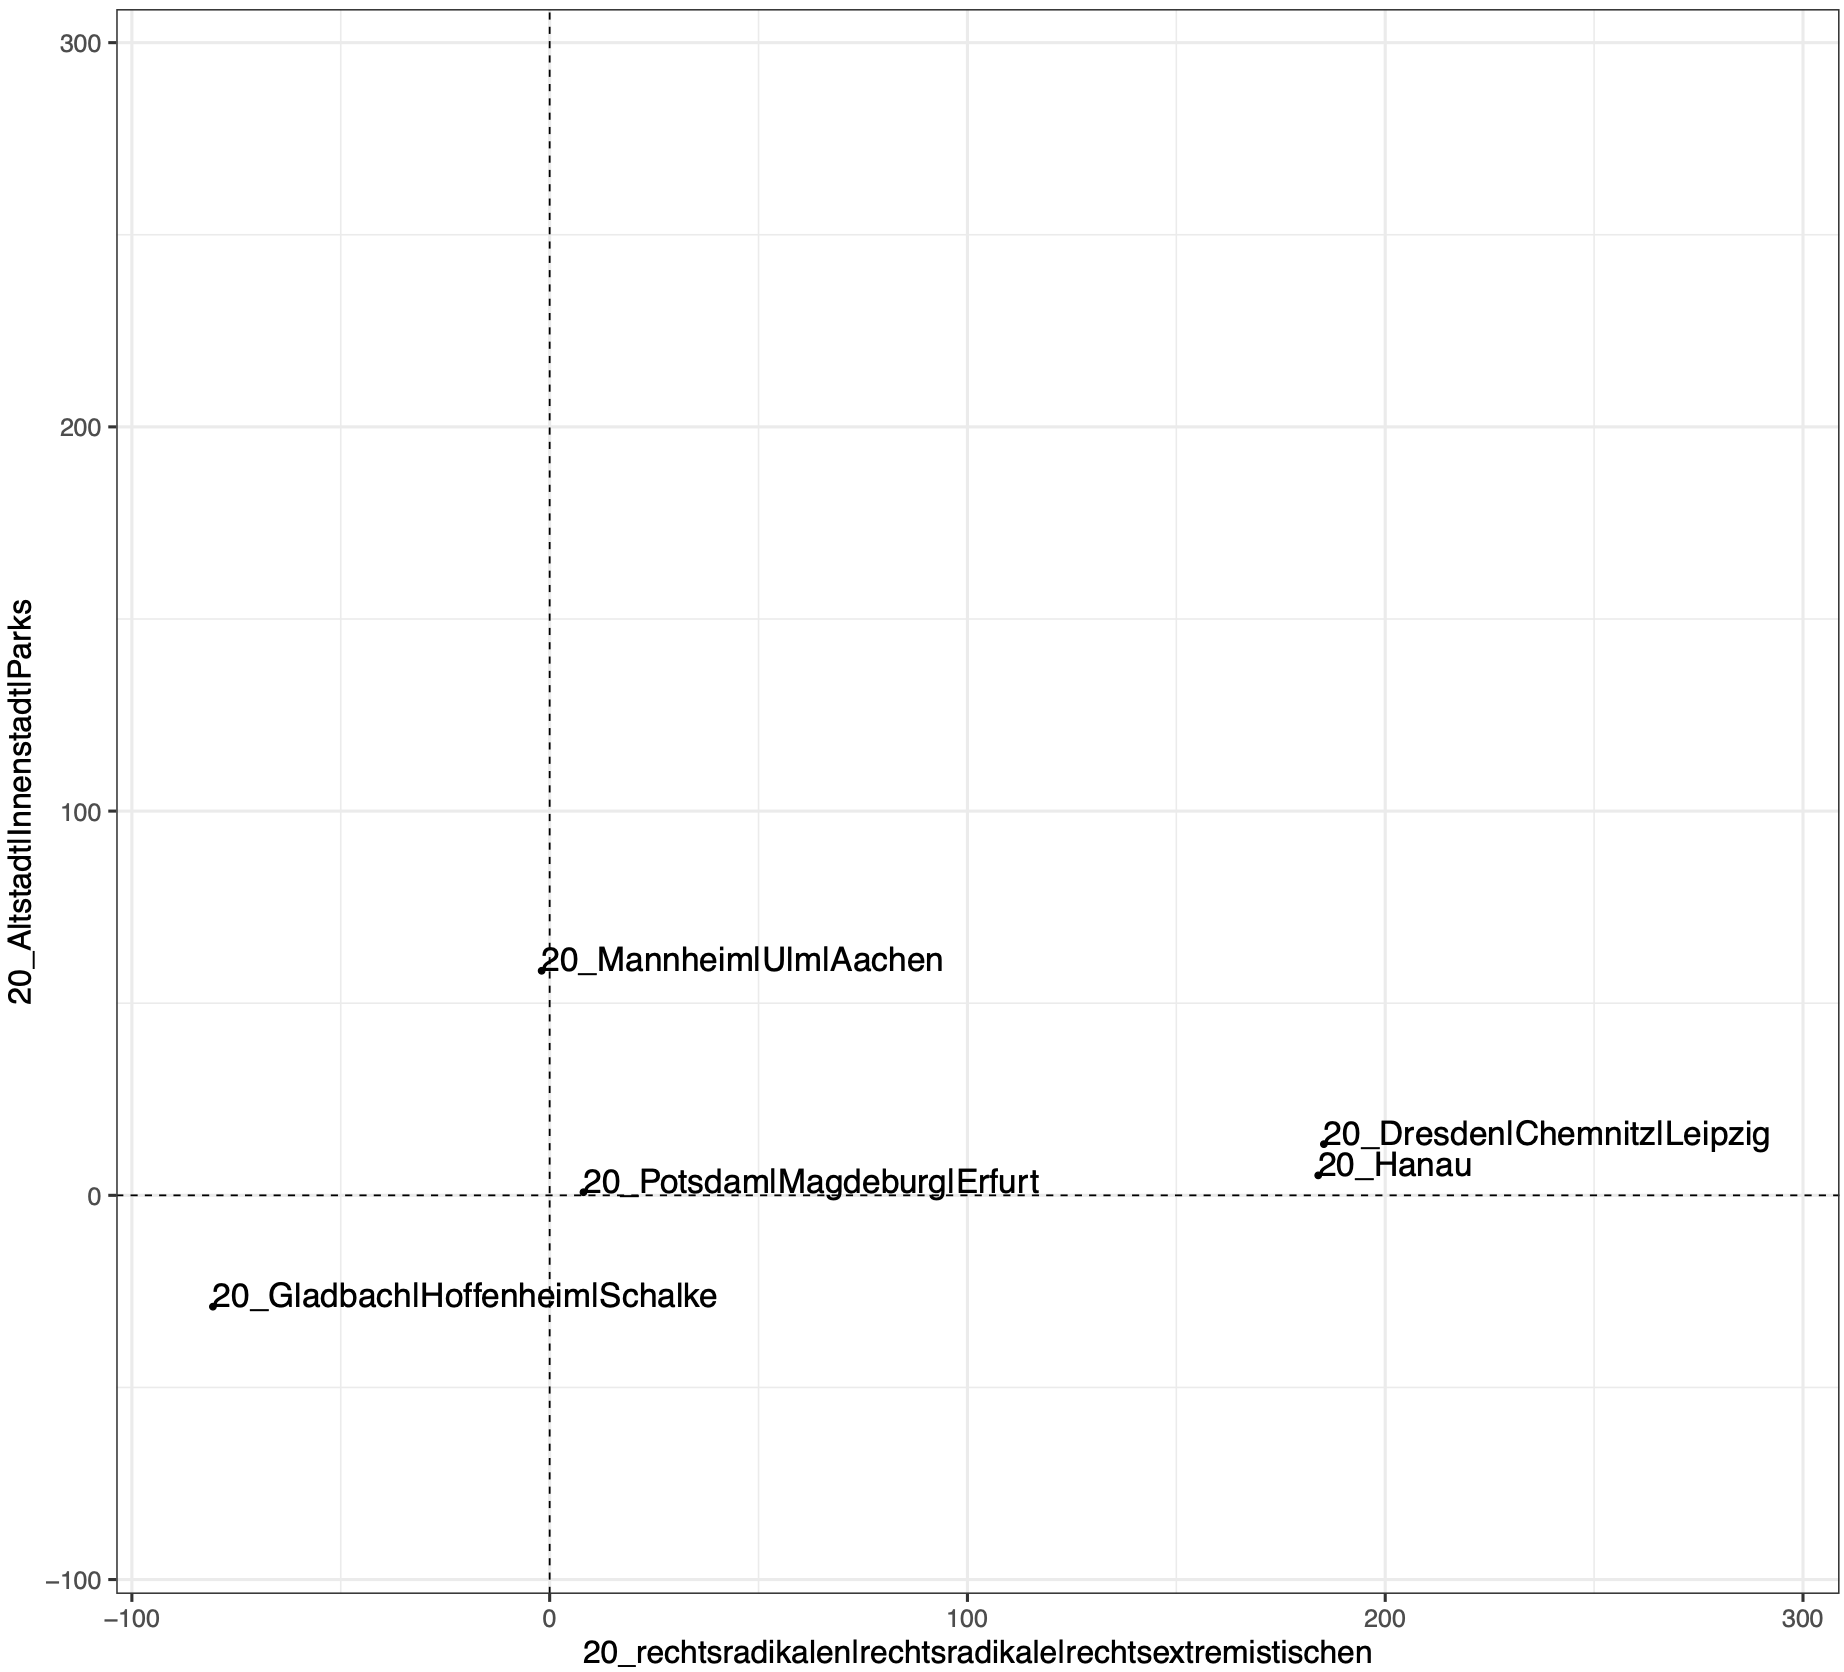
\includegraphics[width=\textwidth]{figures/media/image12.png}
  \caption{\label{fig:staedte-loglikelihood-cluster}Räumliche Darstellung der \emph{Log-Likelihood}-Werte der Städte im Verhältnis zu zwei Clustern aus \tabref{tab:collocation_matrix}.}
\end{figure}

Zu beachten ist, dass zur Messung der Distanz von Word Embeddings in der Regel die Cosinus-Distanz verwendet wird, d.\,h. es wird der Winkel zwischen zwei Punkten im Vektorraum gemessen, nicht ihr ‚direkter` Abstand (euklidische Distanz). Das Cluster \cluster{20\_Potsdam{\breakbar}Magedburg{\breakbar}Erfurt} ist also nur im Sinne der euklidischen Distanz näher an \cluster{20\_Gladbach{\breakbar}Hoffenheim{\breakbar}Schalke} als an \cluster{20\_Hanau} und \cluster{20\_Dresden{\breakbar}Chemnitz{\breakbar}Leipzig}.\footnote{Es sei außerdem noch einmal betont, dass diese Ausführungen nur illustrativen Charakter haben. Zwar approximieren auf klassischen Kollokationen (PMI) beruhende Vektoren durchaus W\emph{ord2Vec}-Skip-Gram-Vektoren \autocite{levyNeuralWordEmbedding2014}. Die tatsächliche Berechnung von neuronalen Word Embeddings, wie in der folgenden Analyse vorgenommen, unterscheidet sich jedoch wesentlich (siehe Kapitel \ref{wie-funktioniert-die-berechnung-von-word-embeddings}).} Misst man hingegen die Cosinus-Distanz, sind sich die Cluster \cluster{20\_Potsdam{\breakbar}Magedburg{\breakbar}Erfurt}, \cluster{20\_Hanau} und \cluster{20\_Dresden{\breakbar}Chemnitz{\breakbar}Leipzig} sehr nahe, da ihre Vektoren vom Koordinatenursprung aus in eine ähnliche Richtung zeigen, während das Cluster \cluster{20\_Gladbach{\breakbar}Hoffenheim{\breakbar}Schalke} von ihnen am weitesten entfernt ist.

Betrachtet man Nachbarschaften von Wörtern im Vektorraum, wird die paradigmatische Relation, die Distanzen in ebendiesem zugrunde liegt, deutlich. So sind die nächsten Nachbarn zum Wort \emph{gesund} im Teilkorpus 2020--2021 etwa \emph{fit}, \emph{krank}, \emph{topfit}, \emph{symptomfrei} und \emph{wohlauf}, also Wörter, die in einer teilsynonymen oder antonymen Beziehung zum Ausgangswort stehen. Was an diesem Beispiel ebenfalls deutlich wird, ist der Einfluss des Korpus, auf dem die Embeddings trainiert wurden. So ist \emph{symptomfrei} im vorigen Zeitraum 2017--2019 nicht unter den nächsten Nachbarn des Wortes, dafür finden sich die Ausdrücke \emph{ungesund}, \emph{schmerzfrei}, \emph{gesünder}, \emph{hungrig} und \emph{fit} als fünf nächste Nachbarn, was anzeigt, dass es hier viel mehr um Fragen des \emph{gesunden} Lebensstils bzw. anderersartige Krankheiten (\emph{schmerzfrei}) geht als während der Corona-Pandemie. Word Embeddings repräsentieren also nicht einfach eine kontextabstrakte Bedeutung im Sinne einer lexikalischen Semantik, die pragmatische Aspekte ausklammert. Während es sinnvoll erscheinen könnte, sehr große und in Hinblick auf unterschiedliche Strata ausgewogene Referenzkorpora zu verwenden, um solche kontextuellen semantischen Verschiebungen zu nivellieren, ist dies gerade in korpuspragmatischen Ansätzen nicht sinnvoll. Word Embeddings stellen hier, gerade weil sich Kontexte in sie einschreiben, ein hervorragendes Mittel dar, um kontextbedingte diskursive Veränderungen -- operationalisiert als Subkorpora -- analysieren zu können. Unterschiede, die sich durch die Wahl des Korpus bzw. Subkorpus ergeben, sind hier also kein Stichprobenproblem, sondern intendierte Datengrundlage für die Analyse \autocite[siehe auch][217-218]{knuchelMachineLearningUnd2023}.

Mithilfe von Word-Embeddings gelingt es also, einen von Tognini-Bonelli zentral gesetzten methodischen Schritt des \emph{corpus-driven} Vorgehens systematisch für jeden Type des Korpus durchzuführen, nämlich die Analyse von Konkordanzen auf der vertikalen Achse in Hinblick auf Muster (hier: im Kotext vorkommende Wörter) und diese nur in der Zusammenschau ersichtlichen Muster als für das Sprachsystem unmittelbar relevant zu deuten:

\begin{quote}
The patterns on the vertical axis are the patterns of \emph{langue} and these are just as physical and concrete as those of \emph{parole}, but they could not be observed until the instances were gathered together - until the advent of computer corpora. The theorists of the earlier part of last century thought that the organisation of \emph{langue} was abstract and unobservable, but that position was an indication of the state of the technology and not the state of the language. The \emph{langue} of Italian, as it relates to the profile of \emph{saper} and of \emph{sapere}, for instance, is there on the page, every bit as physically present as each of its component utterances. \autocite[98-99]{tognini-bonelliCorpusLinguisticsWork2001}
\end{quote}

Im Vergleich zum Vorgehen bei Tognini-Bonelli, das noch auf der Betrachtung von Konkordanzlisten zu einzelnen Suchanfragen beruhte, hat die Technologie nun erneut einen großen Schritt gemacht und das Type-Inventar ganzer Korpora kann auf syntagmatische Gebrauchsmuster untersucht werden.

\subsubsubsection{Wie funktioniert die Berechnung von Word Embeddings?}\label{wie-funktioniert-die-berechnung-von-word-embeddings}

% Zum Durchbruch verhalfen Word Embeddings die von Mikolov et al. \autocite*{mikolovEfficientEstimationWord2013} bei Google entwickelten \emph{Word2Vec}-Algorithmen, mit denen die Ermittlung der Vektoren effizient und für große Datenmengen mit überschaubarem Hardware-Bedarf möglich wurde. Dabei wird ein neuronales Netz verwendet, mit dessen Hilfe Embeddings mit üblicherweise zwischen 200 und 600 Dimensionen berechnet werden können. Die Anzahl der Dimensionen liegt hier also deutlich unter der des oben zu Zwecken der Illustration skizzierten Beispiels, das die gesamte Type-Anzahl des Korpus als Dimensionen erfordern würde. Die Kehrseite dieses effizienteren Verfahrens ist, dass die einzelnen Werte der Dimensionen nicht unmittelbar interpretierbar sind. Sie stellen nun statt konkreten \emph{latente} semantische Features dar. Eine einzelne Dimension kann also etwas über das Kollokationsverhalten mit einer ganzen (unbekannten) Reihe anderer Wörter aussagen. Die Funktionsweise des neuronalen Netzes im Fall von \emph{Word2Vec} \autocite{mikolovEfficientEstimationWord2013} soll im Folgenden skizziert werden \autocite[siehe ausführlich][]{rongWord2vecParameterLearning2016}. Zunächst ist zwischen zwei Varianten des Algorithmus zu unterscheiden: \emph{Continuous Bag of Words} (CBOW) und \emph{Continuous Skip-gram} (Skip-Gram). Für beide Algorithmen wird das Korpus zunächst tokenisiert und in Sätze gegliedert. Im Anschluss erfolgt ein Training des neuronalen Netzes, indem es Vorhersagen über die Wörter im Satz -- in Abhängigkeit der sie umgebenden Wörter -- treffen muss. Während das Training neuronaler Netze in der Regel ein Trainingsdatenset voraussetzt, in dem die zu lernenden Features bereits (oftmals händisch) annotiert sind, nutzen Word-Embedding-Algorithmen das Korpus selbst als Trainingsgrundlage. Sie maskieren einzelne Wörter und sagen sie in Abhängigkeit anderer sie umgebender Wörter voraus -- kennen dabei ja aber stets die richtige Antwort und können so den Erfolg ihrer Vorhersage bewerten. Im Fall von CBOW wird ein Wort des Satzes maskiert und das Netz muss auf Basis des Kotextes (ein festzulegender Wert von per Default zwei Wörtern zur Linken und Rechten des Fokus-Wortes) vorhersagen, um welches Wort es sich handelt. Bei \emph{SkipGram} wird umgekehrt ein Wort vorgegeben und die Vorhersage erfolgt zum maskierten Kontext. Wesentliche Parameter für den Algorithmus sind die Anzahl der Dimensionen, die Variante (CBOW oder \emph{SkipGram}) und das Kontextfenster. Die Architektur des verwendeten neuronalen Netzes (siehe \figref{fig:cbow-architektur}) umfasst eine Eingabeschicht (\emph{input layer}), eine interne Repräsentation (\emph{projection layer}) sowie eine Ausgabeschicht (\emph{output layer}). Alle \emph{layer} entsprechen Vektoren einer bestimmten Länge und beinhalten Zahlenwerte. \emph{In}- und \emph{output layer} haben die Länge des Korpusvokabulars, während die Länge des \emph{projection layers} der festzulegenden Dimensionsanzahl entspricht.
%
% \begin{figure}[t]
%   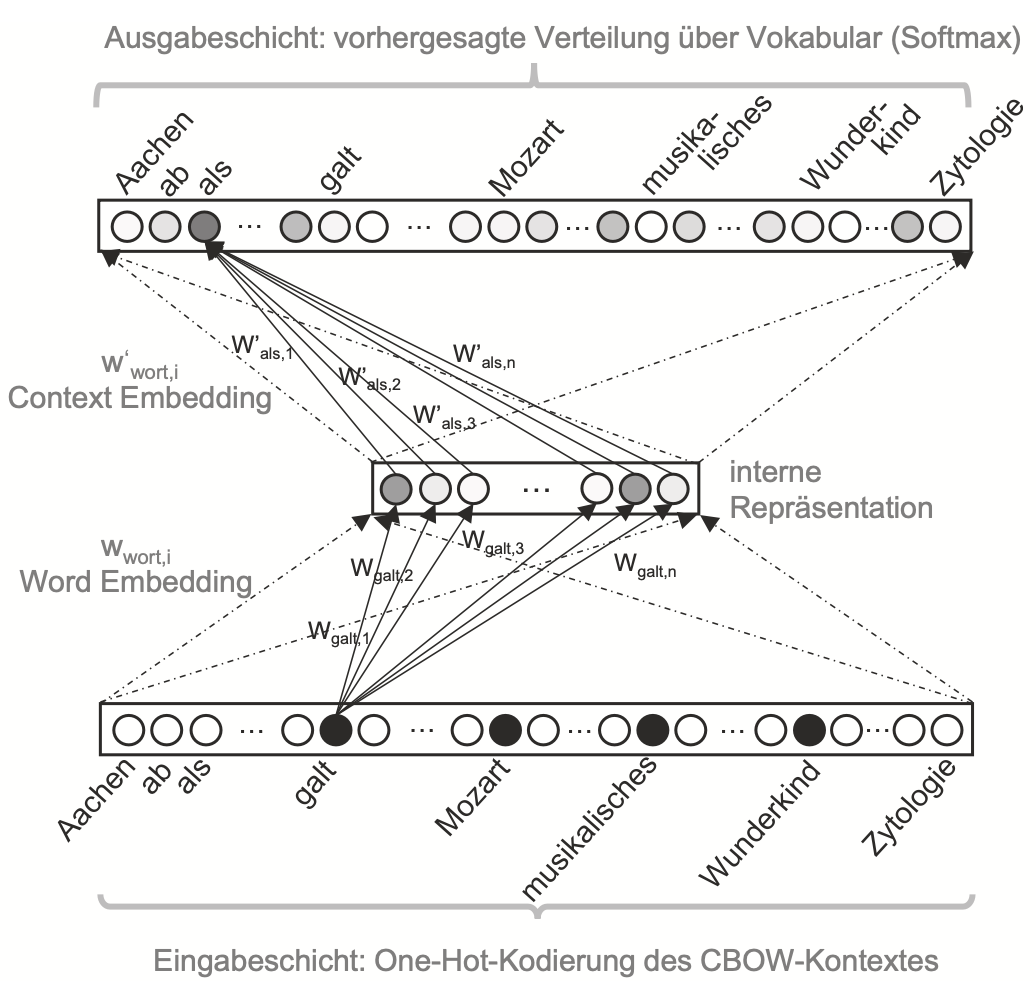
\includegraphics[width=\textwidth]{figures/media/image13.png}
%   \caption{\label{fig:cbow-architektur}Schematische Darstellung der CBOW-Architektur für die Vorhersage von \emph{als} im Satz \emph{Mozart galt als musikalisches Wunderkind} (Abbildung 5.11 aus \citealt[221]{biemannWissensrohstoffTextEinfuehrung2022}).}
% \end{figure}
%
% ~\figref{fig:cbow-architektur} zeigt eine schematische Darstellung für die CBOW-Variante des Algorithmus. Im unteren \emph{input layer} ist ausschnittsweise ein Vektor der Länge des Korpusvokabulars dargestellt, in dem die vier Kontextwörter \emph{galt}, \emph{Mozart}, \emph{musikalisch} und \emph{Wunderkind} markiert sind. Genau genommen verbergen sich dahinter vier Vektoren, jeweils in der Länge des Korpusvokabulars, die an jeder Stelle des Vokabulars eine 0 aufweisen, außer an der Stelle des jeweiligen Kontext-Wortes, das mit 1 markiert ist (sogenannte \emph{One-Hot}-Vektoren). Es finden im Anschluss in zwei Schritten Matrix-Multiplikationen statt: Zunächst wird jeder der vier \emph{One-Hot}-Vektoren mit \emph{n} zufällig initialisierten Werten, den sogenannten Gewichten, multipliziert und das arithmetische Mittel dieser vier Matrix-Multiplikationen (die ‚latente` oder ‚interne Repräsentation`) vom \emph{projection layer} in Richtung \emph{output layer} weitergegeben. Es findet nun erneut eine Matrix-Multiplikation mit zufällig initialisierten Werten statt. Dieses Mal entspricht die Anzahl der Gewichte jedoch der Größe des Vokabulars, d.\,h. der Anzahl der Korpus-Types. Das Ergebnis der Multiplikation sowie der nachfolgenden Anwendung der \emph{softmax}-Funktion\footnote{Mithilfe der \emph{softmax}-Funktion können die Werte von Vektoren in eine Wahrscheinlichhkeitsverteilung überführt werden.} findet sich im \emph{output layer}. Es handelt sich um einen Vektor der Länge des Vokabulars, wobei jeder Wert der Wahrscheinlichkeit des jeweiligen Wortes des Vokabulars in Abhängigkeit der Kontext-Wörter \emph{Mozart}, \emph{galt}, \emph{musikalisches} und \emph{Wunderkind} entspricht (das sogenannte \emph{context embedding}). Durch die dunkle Färbung der Vektordimension zu \emph{als} zeigt die Grafik an, dass das Training bereits fortgeschritten ist und das richtige Wort vorhergesagt wird. Der Ausgabevektor wird sodann mit dem Eingabevektor (Zielwort = 1, andere Wörter = 0) abgeglichen und die gemessene Differenz zwischen beiden zur Adjustierung der Gewichte genutzt (\emph{back propagation}). Während die \emph{context embeddings} i.d.R. nicht weiter genutzt werden,\footnote{Siehe aber z.\,B. Fankhauser \& Kupietz \autocite*{fankhauserCountBasedPredictiveLanguage2022}, die mit ihrer Hilfe Kollokationen \emph{prediction-} statt \emph{count-based} berechnen.} finden sich die eigentlichen \emph{n}-dimensionalen Word Embeddings in den Gewichten zwischen \emph{input} und \emph{projection layer}.
%
% \hspace{-1mm} Zu beachten bei der Berechnung bzw. der Interpretation von Word-Embedding-Modellen (WEM) ist, dass ein WEM immer nur in sich schlüssig ist und die Embeddings eines Modells nicht mit denen anderer, unabhängig trainierter, Modelle verglichen werden können. Dies liegt in den Zufallskomponenten begründet, die beim Training des neuronalen Netzes wirksam sind. Man spricht bei diesen Algorithmen von nicht-deterministischen Algorithmen. Im Gegensatz zu ihren deterministischen Äquivalenten liefern sie auch bei gleicher Datengrundlage und gleichen Parametern keine identischen Ergebnisse. Es ist außerdem wichtig, auf eine möglichst große Datengrundlage und mithin eine möglichst große Anzahl an Kotexten für jedes Wort zurückgreifen zu können, um Zufallseinflüsse zu mindern.

Zum Durchbruch verhalfen Word Embeddings die von Mikolov et al. \autocite*{mikolovEfficientEstimationWord2013} bei Google entwickelten \emph{Word2Vec}-Algorithmen, mit denen die Ermittlung der Vektoren effizient und für große Datenmengen mit überschaubarem Hardware-Bedarf möglich wurde. Dabei wird ein neuronales Netz verwendet, mit dessen Hilfe Embeddings mit üblicherweise zwischen 200 und 600 Dimensionen berechnet werden können. Die Anzahl der Dimensionen liegt hier also deutlich unter der des oben zu Zwecken der Illustration skizzierten Beispiels, das die gesamte Type-Anzahl des Korpus als Dimensionen erfordern würde. Die Kehrseite dieses effizienteren Verfahrens ist, dass die einzelnen Werte der Dimensionen nicht unmittelbar interpretierbar sind. Sie stellen nun statt konkreten \emph{latente} semantische Features dar. Eine einzelne Dimension kann also etwas über das Kollokationsverhalten mit einer ganzen (unbekannten) Reihe anderer Wörter aussagen. Die Funktionsweise des neuronalen Netzes im Fall von \emph{Word2Vec} \autocite{mikolovEfficientEstimationWord2013} soll im Folgenden skizziert werden \autocite[siehe ausführlich][]{rongWord2vecParameterLearning2016}. Zunächst ist zwischen zwei Varianten des Algorithmus zu unterscheiden: \emph{Continuous Bag of Words} (CBOW) und \emph{Continuous Skip-gram} (Skip-Gram). Für beide Algorithmen wird das Korpus zunächst tokenisiert und in Sätze gegliedert. Im Anschluss erfolgt ein Training des neuronalen Netzes, indem es Vorhersagen über die Wörter im Satz -- in Abhängigkeit der sie umgebenden Wörter -- treffen muss. Während das Training neuronaler Netze in der Regel ein Trainingsdatenset voraussetzt, in dem die zu lernenden Features bereits (oftmals händisch) annotiert sind, nutzen Word-Embedding-Algorithmen das Korpus selbst als Trainingsgrundlage. Sie maskieren einzelne Wörter und sagen sie in Abhängigkeit anderer sie umgebender Wörter voraus -- kennen dabei ja aber stets die richtige Antwort und können so den Erfolg ihrer Vorhersage bewerten. Im Fall von CBOW wird ein Wort des Satzes maskiert und das Netz muss auf Basis des Kotextes (ein festzulegender Wert von per Default fünf Wörtern zur Linken und Rechten des Fokus-Wortes) vorhersagen, um welches Wort es sich handelt. Bei \emph{SkipGram} wird umgekehrt ein Wort vorgegeben und die Vorhersage erfolgt zum maskierten Kontext. Wesentliche Parameter für den Algorithmus sind die Anzahl der Dimensionen, die Variante (CBOW oder \emph{SkipGram}) und das Kontextfenster. Die Architektur des verwendeten neuronalen Netzes (siehe \figref{fig:cbow-architektur}) umfasst eine Eingabeschicht (\emph{input layer}), eine interne Repräsentation (\emph{projection layer}) sowie eine Ausgabeschicht (\emph{output layer}). Alle \emph{layer} entsprechen Vektoren einer bestimmten Länge und beinhalten Zahlenwerte. \emph{In}- und \emph{output layer} haben die Länge des Korpusvokabulars, während die Länge des \emph{projection layers} der festzulegenden Dimensionsanzahl entspricht.

\begin{figure}[t]
  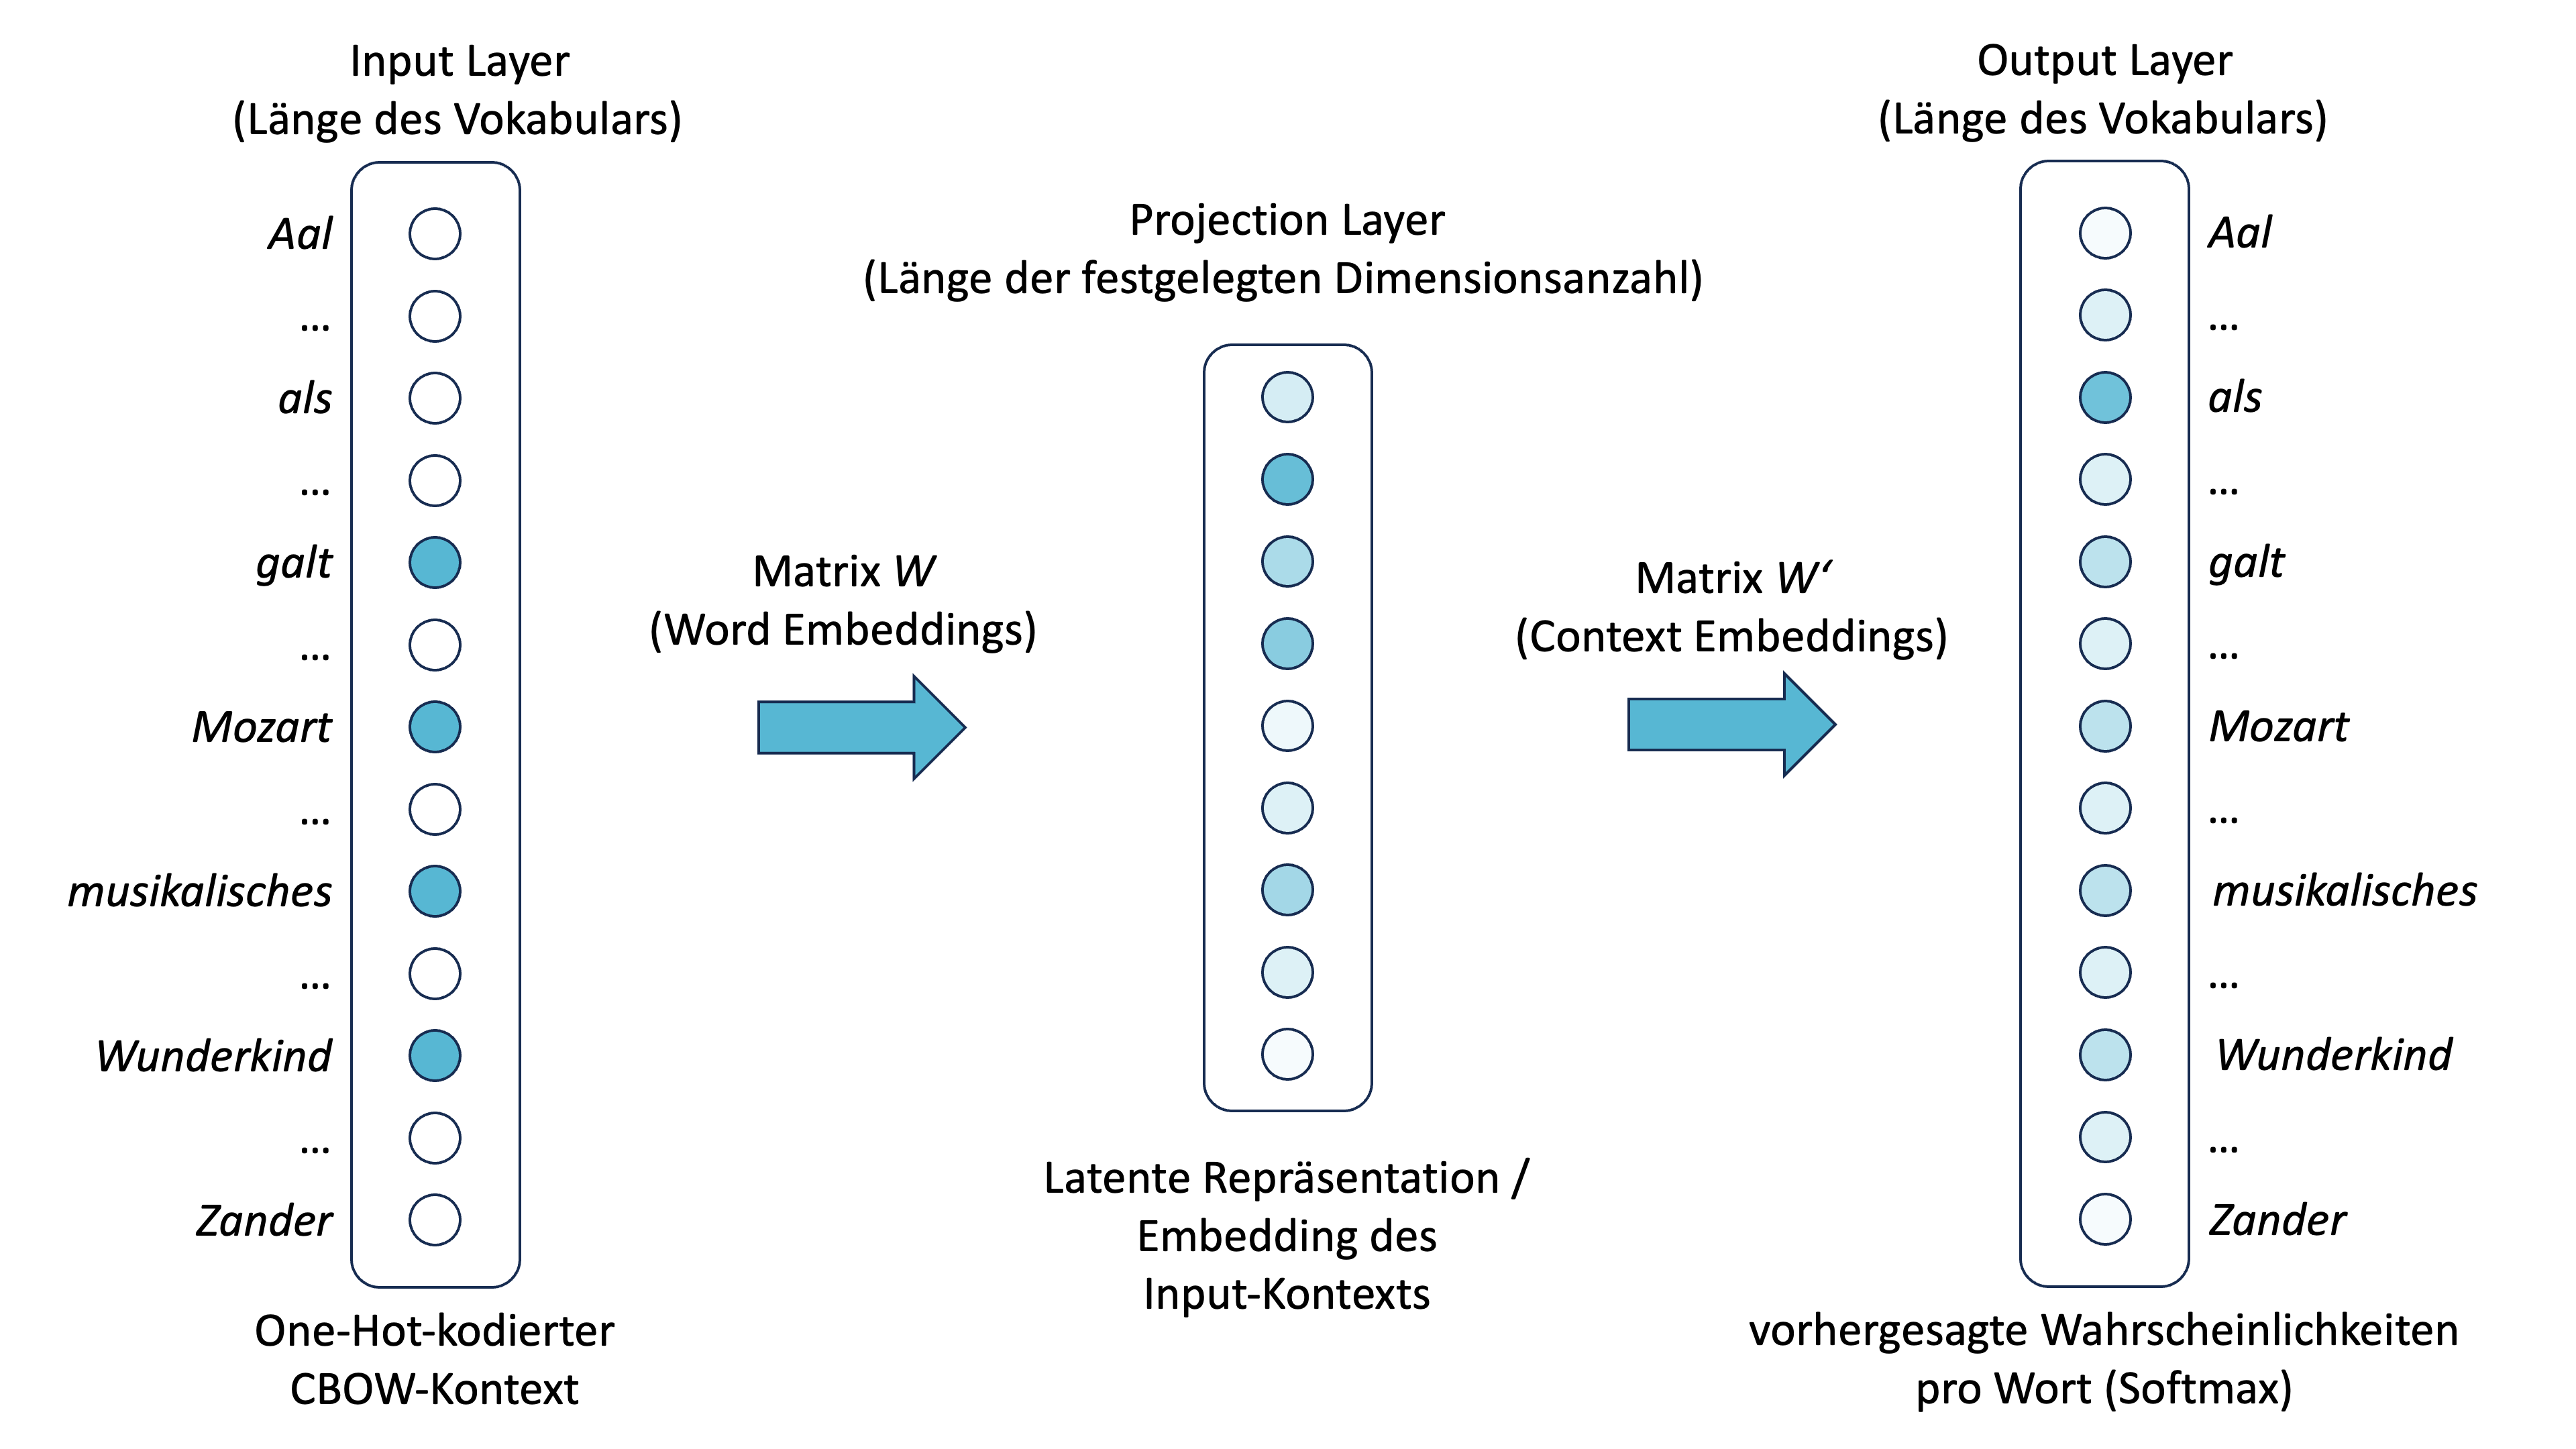
\includegraphics[width=\textwidth]{figures/media/grafik_cbow.png}
  \caption{\label{fig:cbow-architektur}Schematische Darstellung der CBOW-Architektur für die Vorhersage von \emph{als} im Satz \emph{Mozart galt als musikalisches Wunderkind} (Adaption von Abbildung 5.11 aus \citealt[221]{biemannWissensrohstoffTextEinfuehrung2022}).}
\end{figure}

~\figref{fig:cbow-architektur} zeigt eine schematische Darstellung für die CBOW-Variante des Algorithmus. Im unteren \emph{input layer} ist ausschnittsweise ein Vektor der Länge des Korpusvokabulars dargestellt, in dem die vier Kontextwörter \emph{galt}, \emph{Mozart}, \emph{musikalisch} und \emph{Wunderkind} markiert sind. Genau genommen verbergen sich dahinter vier Vektoren, jeweils in der Länge des Korpusvokabulars, die an jeder Stelle des Vokabulars eine 0 aufweisen, außer an der Stelle des jeweiligen Kontext-Wortes, das mit 1 markiert ist (sogenannte \emph{One-Hot}-Vektoren). Es finden im Anschluss in zwei Schritten Matrix-Multiplikationen (\emph{W} und \emph{W'}) statt: Zunächst wird jeder der vier \emph{One-Hot}-Vektoren mit \emph{n} zufällig initialisierten Werten, den sogenannten Gewichten, multipliziert und das arithmetische Mittel dieser vier Matrix-Multiplikationen (die ‚latente` oder ‚interne Repräsentation`) vom \emph{projection layer} in Richtung \emph{output layer} weitergegeben. Es findet nun erneut eine Matrix-Multiplikation mit zufällig initialisierten Werten statt. Dieses Mal entspricht die Anzahl der Gewichte jedoch der Größe des Vokabulars, d.\,h. der Anzahl der Korpus-Types. Das Ergebnis der Multiplikation sowie der nachfolgenden Anwendung der \emph{softmax}-Funktion\footnote{Mithilfe der \emph{softmax}-Funktion können die Werte von Vektoren in eine Wahrscheinlichhkeitsverteilung überführt werden.} findet sich im \emph{output layer}. Es handelt sich um einen Vektor der Länge des Vokabulars, wobei jeder Wert der Wahrscheinlichkeit des jeweiligen Wortes des Vokabulars in Abhängigkeit der Kontext-Wörter \emph{Mozart}, \emph{galt}, \emph{musikalisches} und \emph{Wunderkind} entspricht. Durch die dunkle Färbung der Vektordimension zu \emph{als} zeigt die Grafik an, dass das Training bereits fortgeschritten ist und das richtige Wort vorhergesagt wird. Der Ausgabevektor wird sodann mit dem Eingabevektor (Zielwort = 1, andere Wörter = 0) abgeglichen und die gemessene Differenz zwischen beiden zur Adjustierung der Gewichte genutzt (\emph{back propagation}). Während die \emph{context embeddings} i.d.R. nicht weiter genutzt werden,\footnote{Siehe aber z.\,B. Fankhauser \& Kupietz \autocite*{fankhauserCountBasedPredictiveLanguage2022}, die mit ihrer Hilfe Kollokationen \emph{prediction-} statt \emph{count-based} berechnen.} finden sich die eigentlichen \emph{n}-dimensionalen Word Embeddings in den Gewichten zwischen \emph{input} und \emph{projection layer}, d.h. in Matrix \emph{W}.

\hspace{-1mm} Zu beachten bei der Berechnung bzw. der Interpretation von Word-Embedding-Modellen (WEM) ist, dass ein WEM immer nur in sich schlüssig ist und die Embeddings eines Modells nicht mit denen anderer, unabhängig trainierter, Modelle verglichen werden können. Dies liegt in den Zufallskomponenten begründet, die beim Training des neuronalen Netzes wirksam sind. Man spricht bei diesen Algorithmen von nicht-deterministischen Algorithmen. Im Gegensatz zu ihren deterministischen Äquivalenten liefern sie auch bei gleicher Datengrundlage und gleichen Parametern keine identischen Ergebnisse. Es ist außerdem wichtig, auf eine möglichst große Datengrundlage und mithin eine möglichst große Anzahl an Kotexten für jedes Wort zurückgreifen zu können, um Zufallseinflüsse zu mindern.

\subsubsubsection{Vergleichbarkeit von Word-Embedding-Modellen}\label{vergleichbarkeit-von-word-embedding-modellen}

Um das Problem der Nicht-Vergleichbarkeit unabhängig trainierter Word-Embedding-Modelle zu lösen, wurden in der Computerlinguistik unterschiedliche Lösungsansätze entwickelt \autocites[siehe etwa][]{dubossarskyBottomApproachCategory2015, fankhauserAnalyzingDomainSpecific2019, yaoDynamicWordEmbeddings2018, dicarloTrainingTemporalWord2019}. Aufgrund der guten Performance-Werte sowie der einfachen Handhabbarkeit des Algorithmus verwende ich die Erweiterung des \emph{Word2Vec} Algorithmus \emph{Temporal Word Embeddings with a Compass} (TWEC) von Di Carlo et al. \autocite*{dicarloTrainingTemporalWord2019}, die das Training von WEM im gleichen Vektorraum für unterschiedliche Subkorpora erlaubt. Die Funktionsweise von TWEC lässt sich wie folgt skizzieren: Zunächst wird ein reguläres Word-Embedding-Modell (der sogenannte \emph{compass}) auf dem gesamten Korpus trainiert, wobei die CBOW-Variante von \emph{Word2Vec} zum Einsatz kommt. Im Anschluss wird die fertig trainierte zweite Matrix des neuronalen Netzes eingefroren und für das Training aller weiteren Modelle für Subkorpora desselben Korpus (sogenannte \emph{slices}) verwendet. Aktualisiert werden dabei dann nur noch die Gewichte zwischen \emph{input} und \emph{projection layer} was dazu führt, dass die resultierenden Wortvektoren zwar in den gleichen Vektorraum eingebettet, jedoch kontextspezifisch trainiert sind. \tabref{tab:diachronic_neighbors} führt die jeweils nächsten Nachbarn zu einzelnen Word Embeddings in unterschiedlichen mit TWEC berechneten diachronen Modellen auf. Fixiert ist jeweils der Ursprungskontext der Wörter. Es werden also z.\,B. in der ersten Zeile nicht die nächsten Nachbarn des Ausdrucks \emph{Querdenker} in den unterschiedlichen Teilkorpora abgefragt, was auch ohne alignierte Modelle möglich wäre, sondern die nächsten Nachbarn zu dem Punkt im semantischen Raum, an dem \emph{Querdenker} in den Jahren 1999--2001 lag. Es handelt sich also um eine onomasiologische statt einer semasiologischen Analyserichtung. Während sich diese Bedeutung kaum verändert hat -- es fällt allerdings auf, dass \emph{Querdenker} selbst im Jahr 2020--2021 nicht mehr an diesem Punkt auftaucht --, zeigt sich an der Abfrage des gleichen Wortes mit Ursprungskontext 2020--2021 ein gänzlich anderes Bild und mithin der Bedeutungswandel des Wortes in der Coronapandemie. Es wird ersichtlich, dass es mithilfe der Methode sehr gut gelingt, Bedeutungswandel einzelner Wörter zu erfassen. Es eröffnet sich zudem eine datengeleitete Zugriffsmöglichkeit auf dieses Phänomen, indem etwa im Vergleich zweier diachroner Word-Embedding-Modelle abgefragt werden kann, welche Wörter die größte Distanz im Vektorraum vom einen zum anderen Zeitpunkt zurückgelegt haben.

\begin{sidewaystable}\small
\caption{Nächste Nachbarn einzelner Embeddings mit Cosinus-Ähnlichkeit im zeitlichen Verlauf.}
\label{tab:diachronic_neighbors}
 \begin{tabularx}{\textwidth}{>{\hsize=0.8\hsize}Q >{\hsize=1.066\hsize}Q >{\hsize=1.066\hsize}Q >{\hsize=1.066\hsize}Q}
  \lsptoprule
  Ausgangsvektor & 1999--2001 & 2011--2013 & 2020--2021 \\
  \midrule
  \emph{Querdenker (99--01)} & \emph{Querdenker} (1.0), \emph{Pragmatiker} (0.73), \emph{Provokateur} (0.71), \emph{Selbstdarsteller} (0.69), \emph{Querkopf} (0.68) & \emph{Querdenker} (0.76), \emph{Netzwerker} (0.73), \emph{Freigeist} (0.70), \emph{Vordenker} (0.69), \emph{Pragmatiker} (0.69) & \emph{Pragmatiker} (0.66), \emph{Netzwerker} (0.66), \emph{Vordenker} (0.66), \emph{Liberaler} (0.65), \emph{Intellektueller} (0.64) \\
  \emph{Querdenker (20--21)} & \emph{Autonome} (0.75), \emph{Rechtsextreme} (0.70), \emph{Neonazis} (0.70), \emph{Rechtsextremen} (0.69), \emph{Rechtsradikale} (0.68) & \emph{Rechtsextreme} (0.73), \emph{Rechtsradikale} (0.71), \emph{Burschenschafter} (0.70), \emph{gewaltbereite} (0.70), \emph{Islamfeinde} (0.68) & \emph{Querdenker} (1.0), \emph{Coronaleugner} (0.80), \emph{Reichsbürger} (0.79), \emph{Corona-Leugner} (0.79), \emph{Impfgegner} (0.78) \\
  \emph{Hanau (20--21)} & \emph{Mölln} (0.63), \emph{Guben} (0.63), \emph{Rostock-lichtenhagen} (0.59), \emph{Solingen} (0.58), \emph{Düsseldorfer\_Synagoge} (0.57) & \emph{Mölln} (0.70), \emph{Solingen} (0.66), \emph{Rostock-lichtenhagen} (0.65), \emph{Newtown} (0.61), \emph{Lichtenhagen} (0.59) & \emph{Hanau} (1.0), \emph{Christchurch} (0.66), \emph{Mölln} (0.66), \emph{Hanauer} (0.64), \emph{Anschlag} (0.64) \\
  \emph{Björn\_Höcke (20--21)} & \emph{Christian\_Worch} (0.67), \emph{Horst\_Mahler} (0.65), \emph{NPD} (0.64), \emph{Aktionsbüro\_Norddeutschland} (0.63), \emph{Reps} (0.63) & \emph{Holger\_Apfel} (0.81), \emph{Udo\_Pastörs} (0.79), \emph{Udo\_Voigt} (0.77), \emph{Pastörs} (0.73), \emph{NPD-Kader} (0.72) & \emph{Björn\_Höcke} (1.0), \emph{Höcke} (0.88), \emph{Andreas\_Kalbitz} (0.85), \emph{Jörg\_Meuthen} (0.80), \emph{Thüringer\_AfD-Chef\_Björn\_Höcke} (0.79) \\
  \emph{Bin\_Laden (02--04)} & \emph{Bin\_Laden} (0.94), \emph{Osama\_Bin\_Laden} (0.90), \emph{Ussama\_Bin\_Laden} (0.87), \emph{bin\_Laden} (0.85), \emph{al-Qaida} (0.80) & \emph{Bin\_Laden} (0.86), \emph{bin\_Laden} (0.82), \emph{al-Qaida} (0.81), \emph{Osama\_Bin\_Laden} (0.76), \emph{Al-Qaida-Chef} (0.75) & \emph{al-Qaida} (0.69), \emph{Terroristen} (0.66), \emph{Soleimani} (0.64), \emph{iS} (0.64), \emph{Al-Qaida} (0.64) \\
  \lspbottomrule
 \end{tabularx}
\end{sidewaystable}

\subsubsubsection{Clustering von Word Embeddings}\label{clustering-von-word-embeddings}
\largerpage
Um Wörter nach ihrer paradigmatischen distributionellen Ähnlichkeit systematisch zusammenfassen und mithin FE induktiv erschließen zu können, bietet sich ein Clustering der berechneten Word Embeddings an, das in der Diskurslinguistik bereits erfolgreich angewandt wurde (siehe \chapref{distributionell-semantische-methodik}). Zum Clustering von Vektoren steht eine Vielzahl unterschiedlicher Algorithmen bereit, die jeweils unterschiedliche Vor- und Nachteile in Hinblick auf die bearbeitbare Datenmenge, die Laufzeit des Algorithmus, oder die Notwendigkeit, eine bestimmte Cluster-Anzahl vorab festzulegen, bieten.\footnote{Eine anschauliche Übersicht zu unterschiedlichen Clustering-Algorithmen steht unter \url{https://scikit-learn.org/stable/modules/clustering.html} zur Verfügung {[}18.12.2025{]}.} Gerade aus einer datengeleitet-explorativen Perspektive sind auch hierarchische Clustering-Algorithmen und solche, die keine vordefinierte Anzahl von Clustern benötigen und die Datenpunkte automatisch in Cluster sowie \emph{noise} gliedern, wie z.\,B. HDBSCAN \autocite{campelloDensityBasedClusteringBased2013} interessant. Mit ihnen wurde experimentiert, letztlich wurde jedoch aufgrund der großen Anzahl zu verarbeitender Datenpunkte (bis zu 365\,815 Types im \textsc{Taz}-Subkorpus) entschieden, den \emph{k-Means}-Algorithmus \autocite{macqueenMethodsClassificationAnalysis1967} zu verwenden, der große Datenmengen effizient in eine festgelegte Anzahl von \emph{k} Clustern einteilen kann und sich auch in Bubenhofers Analysen (siehe \chapref{distributionell-semantische-methodik}) bewährt hat. Bei einem \emph{k-Means}-Clustering wird jeder Datenpunkt, d.\,h. jedes Word Embedding, einem einzigen Cluster zugeordnet. Eine vorherige inhaltliche Definition der zu erwartenden Cluster ist jedoch nicht nötig; die Cluster-Erkennung erfolgt allein aufgrund der Verteilung der Datenpunkte, es handelt sich also um einen unüberwachten -- aus korpuslinguistischer Perspektive also \emph{corpus-driven} -- Algorithmus. Die Funktionsweise ist vergleichsweise simpel: Bei der Berechnung werden zunächst \emph{k} zufällige Cluster-Mittelpunkte (Centroids) im Vektorraum festgelegt. Danach werden alle Datenpunkte ihrem nächsten Cluster-Centroid zugeordnet und es wird pro Cluster aus allen zugeordneten Datenpunkten ein neuer Mittelpunkt berechnet. Im Anschluss beginnt der Prozess von vorne und es werden erneut alle Datenpunkte zugeordnet sowie daraufhin neue Centroids berechnet. Der Algorithmus endet, sobald sich die Zuordnung der Datenpunkte zu den Clustern nicht mehr oder nur noch geringfügig ändert. \figref{fig:kmeans-beispiel-k2} illustriert den Algorithmus an einem Beispiel.

\begin{figure}[t]
%   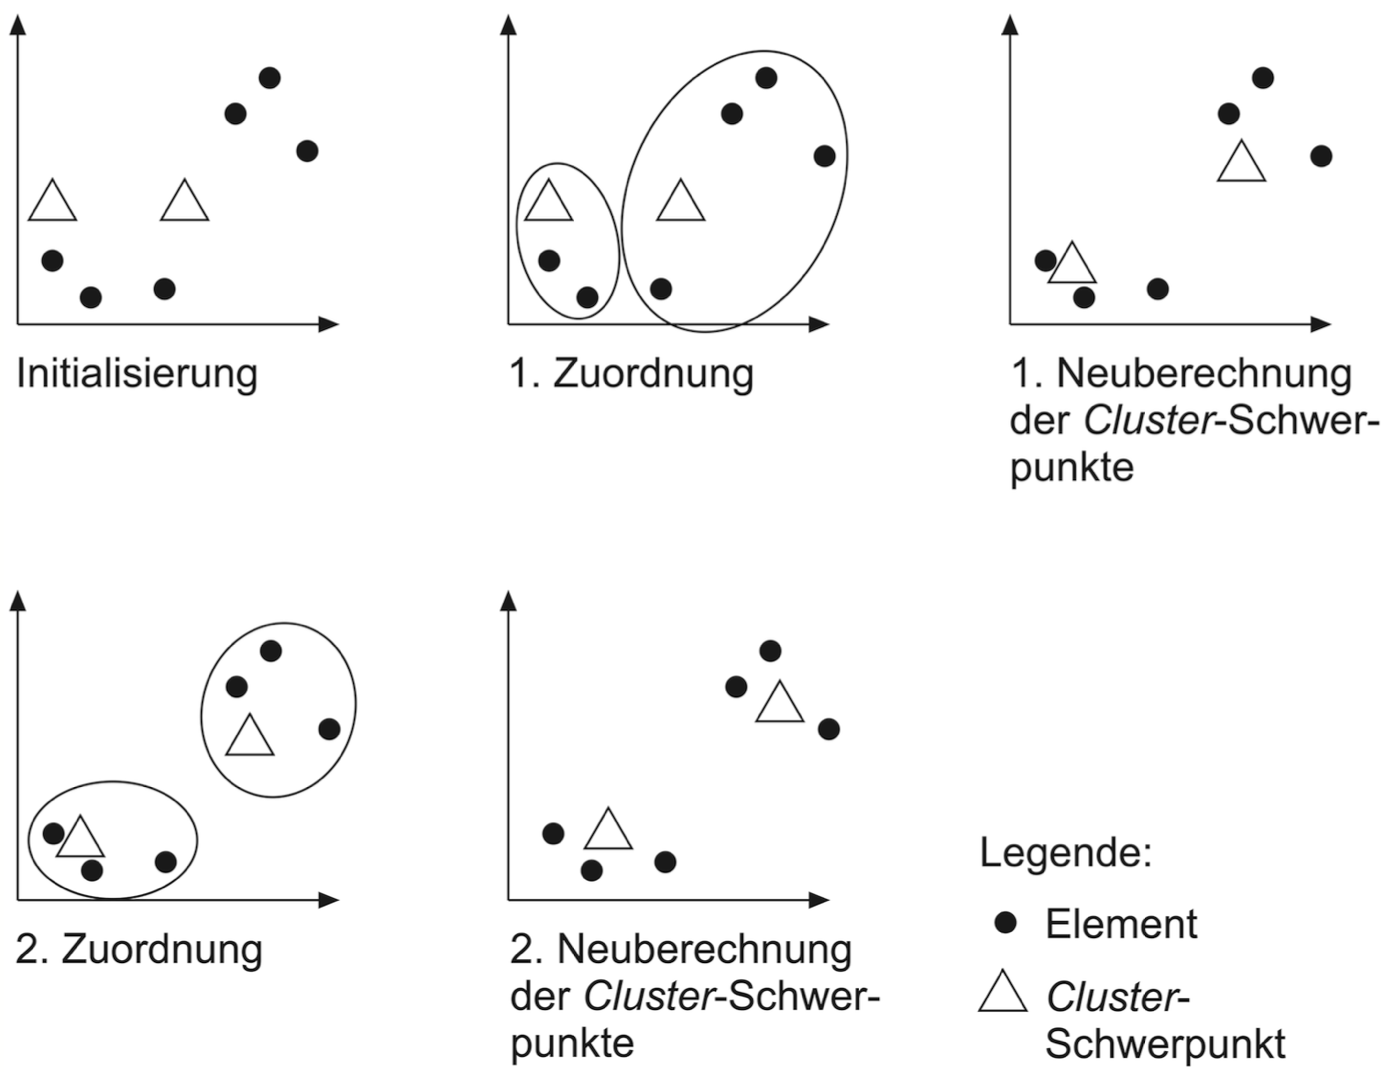
\includegraphics[width=\textwidth]{figures/media/image14.png}
%   \caption{\label{fig:kmeans-beispiel-k2}Illustration des \emph{k-Means}-Algorithmus bei \emph{k} = 2 und sechs Vektoren (Abbildung 6.5 aus \citealt[270]{biemannWissensrohstoffTextEinfuehrung2022}).}
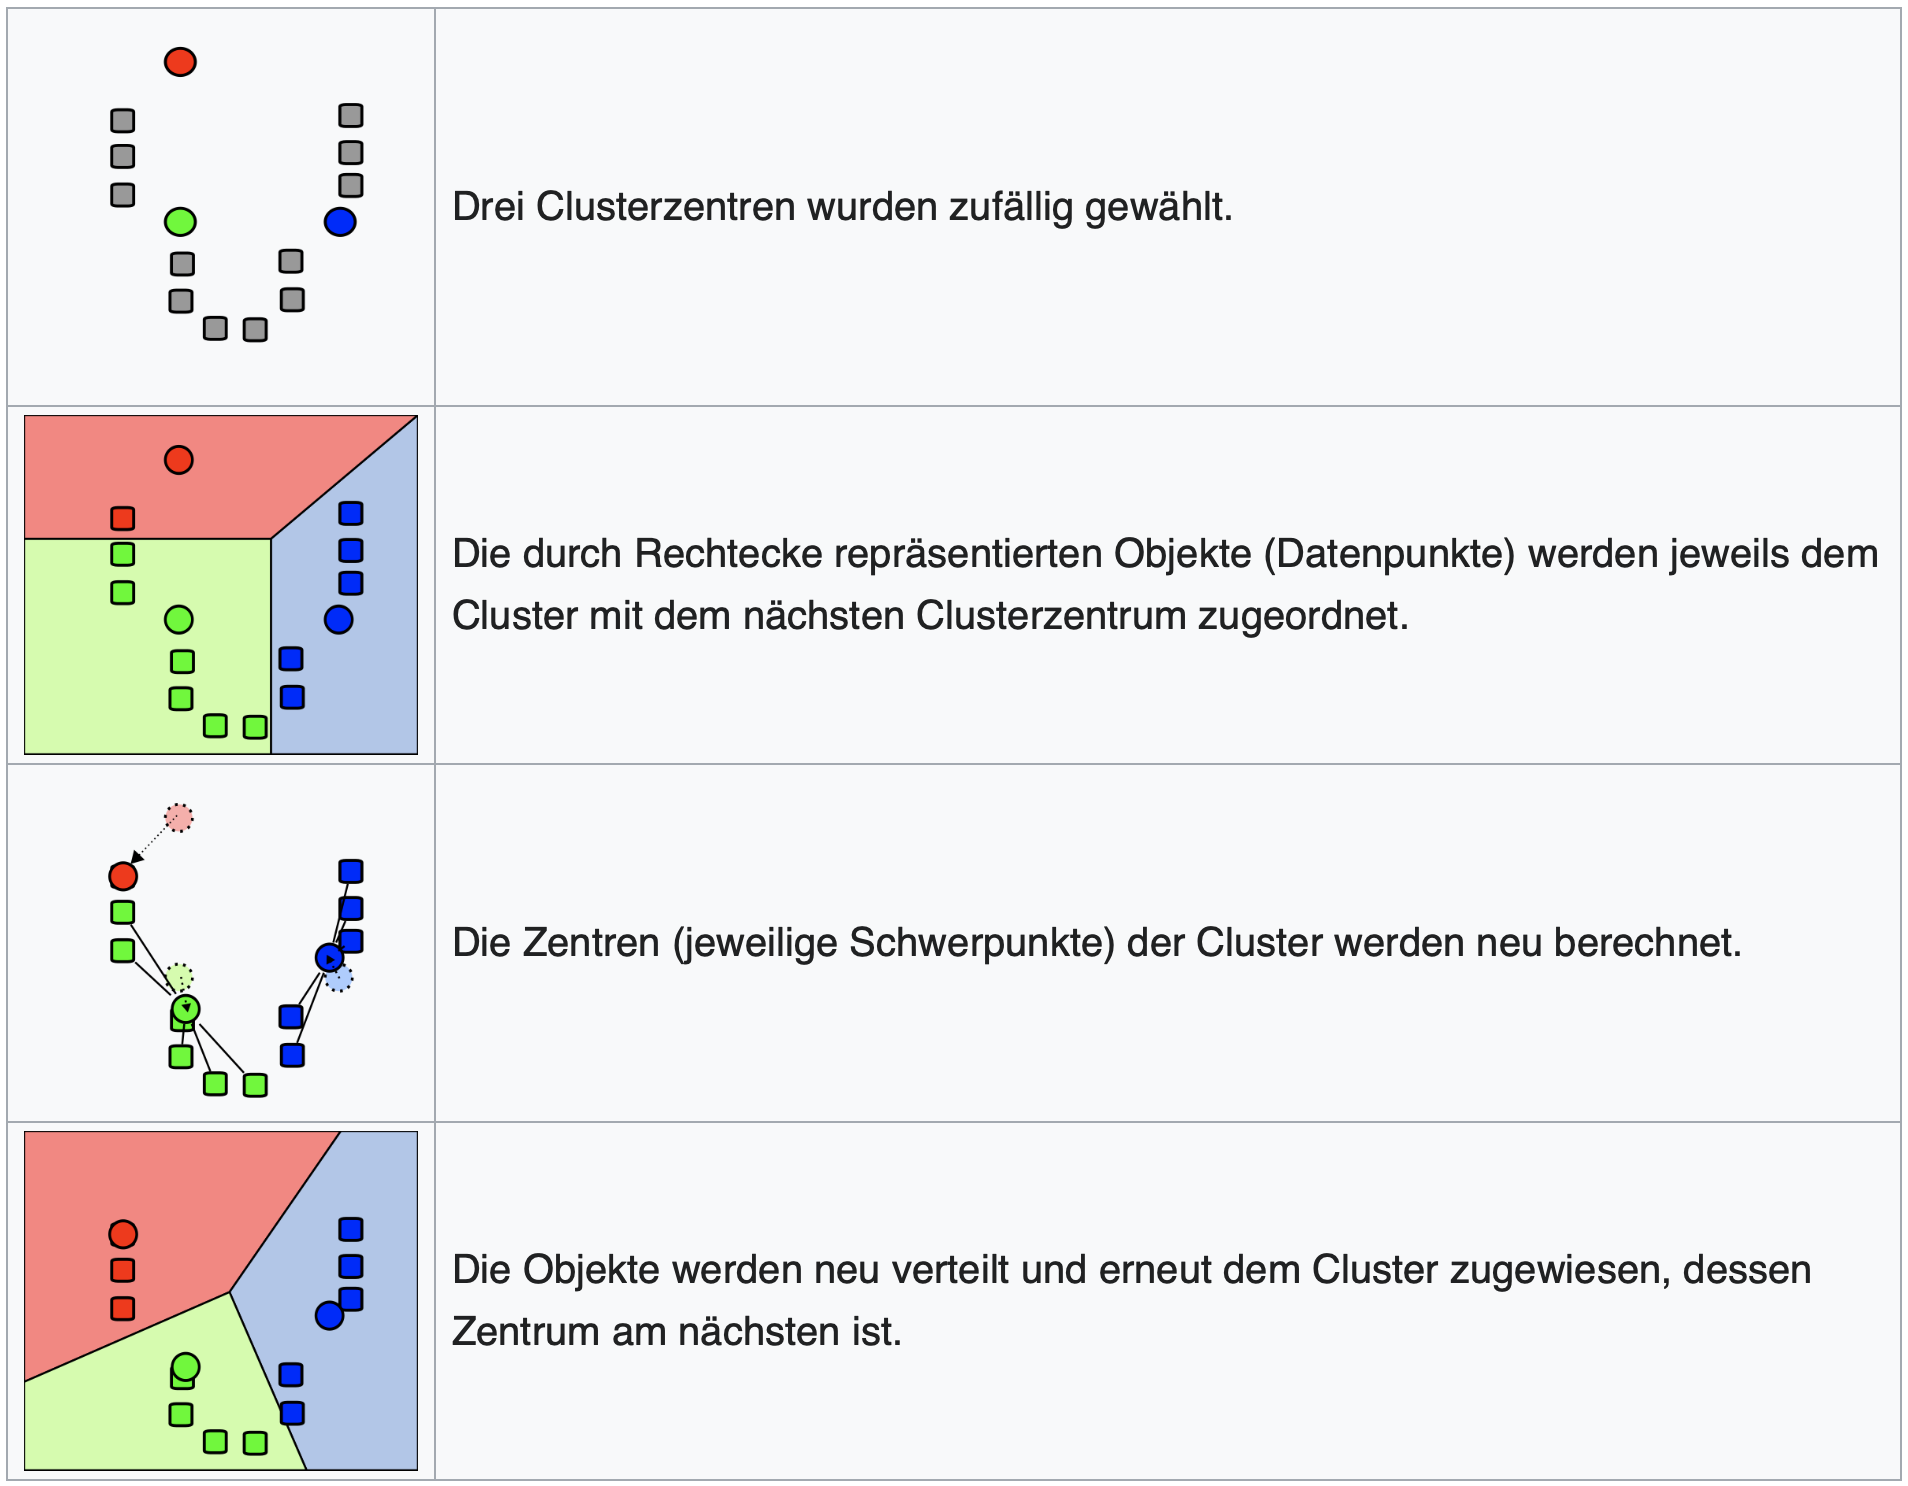
\includegraphics[width=\textwidth]{figures/media/kmeans.png}
  \caption{\label{fig:kmeans-beispiel-k2}Illustration des \emph{k-Means}-Algorithmus bei \emph{k} = 3 und zwölf Vektoren (Urheber der Grafiken: weston.pace, CC BY-SA 3.0, \url{https://de.wikipedia.org/wiki/K-Means-Algorithmus} [31.01.2026]).}
\end{figure}

\largerpage
Durch die Zufallskomponente bei der Initialisierung handelt es sich auch bei \emph{k-Means} um einen nicht-deterministischen Algorithmus, sodass die Zuordnungen der Wörter zu Clustern im Verlauf mehrerer Ausführungen variieren kann. Zu beachten ist darüber hinaus, dass wie Grand et al. \autocite*{grandSemanticProjectionRecovers2022} hervorheben, Nähe von Word Embeddings im Vektorraum immer auf einer globalen semantischen Ähnlichkeit beruht, die sich eigentlich in die Positionierung entlang einer Vielzahl semantischer Dimensionen aufspalten ließe. Je nachdem, was als \emph{tertium comparationis} gewählt ist, können also unterschiedliche Nachbarschaften von Wörtern entstehen. So weisen die Wörter \emph{dolphin} und \emph{tiger} eine geringe Distanz auf, wenn man sie auf die Dimension \emph{size} projiziert; jedoch eine große Distanz bei Projektion auf die Dimension \emph{danger} (siehe \emph{Figure 2a} in \citealt{grandSemanticProjectionRecovers2022}).

%
% \begin{figure}
%   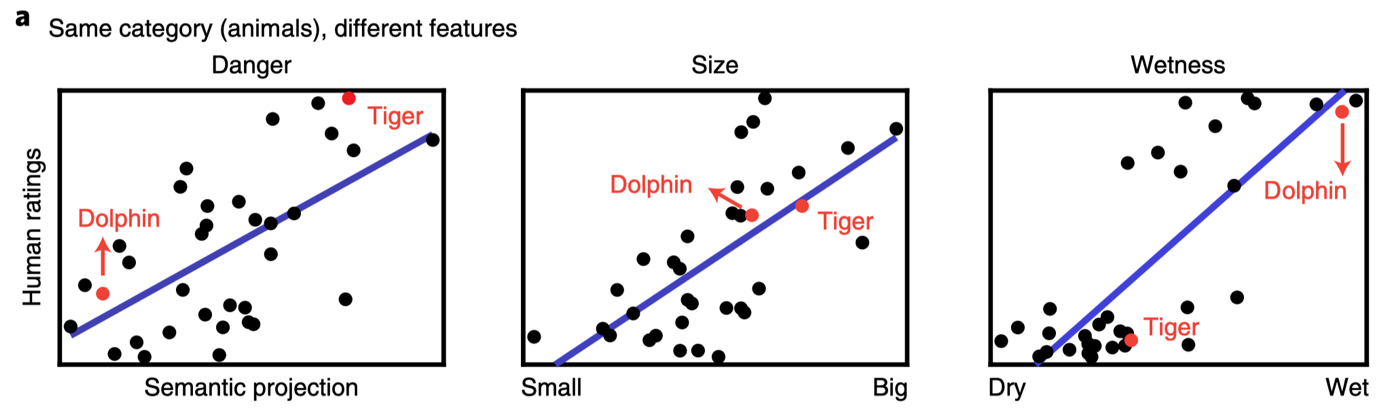
\includegraphics[width=\textwidth]{figures/media/image15.png}
%   \caption{\label{fig:tiere-embeddings-semantik}Korrelation zwischen der Projektion der Word Embeddings unterschiedlicher Tiere auf unterschiedliche semantische Achsen und menschlichen Bewertungen (\emph{Figure 2a} aus \citealt{grandSemanticProjectionRecovers2022}).}
% \end{figure}

Darüber hinaus spielen auch morphosyntaktische Faktoren eine große Rolle bei der Einteilung in Cluster, sodass etwa bestimmte Flexionsformen oder Wortarten häufig im gleichen Cluster anzutreffen sind. Welche semantischen oder morphosyntaktischen Kriterien der Einteilung zugrunde liegen, kann jedoch immer nur im Nachhinein durch Interpretation erschlossen werden und ist Teil der Analyse.

\subsection{Operationalisierung von Frames für distributionelle Methoden}\label{operationalisierung-von-frames-fuer-distributionelle-methoden}

\subsubsection{Geclusterte Word Embeddings als Frame-Elemente}\label{geclusterte-word-embeddings-als-frame-elemente}

Wie im Laufe der Arbeit immer wieder angedeutet, erscheinen korpuslinguistische, auf der Distribution von Wörtern operierende Methoden geeignet, um semantische Frames im Sinne Busses \autocite*{busseFrameSemantikKompendium2012} -- zumindest in Teilen -- induktiv zu erschließen. In diesem Kapitel stelle ich, beginnend mit den Word-Embedding-Clustern, dar, wie ich die über die sprachliche Oberfläche gewonnenen musterhaften Strukturen interpretiere und warum es möglich ist, sie als Elemente semantischer Frames aufzufassen und zu operationalisieren. Zugrunde liegt die Annahme, dass distributionelle, korpuslinguistische Daten „vor einem geistes- und sozialwissenschaftlichen Hintergrund genauso hermeneutisch gedeutet werden müssen wie einzelne Texte`` \autocite[25, siehe ausführlicher \chapref{begriffsklaerungen-quantitativ-und-qualitativ-corpus-driven-und-corpus-based-sowie-die-rolle-von-hermeneutik}]{bubenhoferWennLinguistikKorpuslinguistik2018}.

Wie in den Kapiteln \ref{distributionell-semantische-methodik} und \ref{word-embeddings-als-paradigmatische-distributionelle-muster} ausgeführt, stellen Word-Embeddings eine Möglichkeit dar, die reichhaltige Semantik von Wörtern (Types) eines Korpus zu erfassen, zueinander in Beziehung zu setzen und mithin untersuchbar zu machen. Der semantische Gehalt einzelner Embeddings ist dabei nie unmittelbar abzulesen. Zum einen weil sie, genau wie Wörter, ihre Semantik nur durch ihren Stellenwert im Sinne des Saussureschen \emph{valeur} im gesamten Symbolsystem erhalten \autocite{sahlgrenDistributionalHypothesis2008}; zum anderen weil die mathematischen Dimensionen der Vektoren nicht mit (interpretierbaren) semantischen Dimensionen gleichzusetzen sind, sondern latente Features darstellen \autocite[156-157]{lenciDistributionalModelsWord2018}. Um die Semantik von Word-Embeddings zu erschließen, ist es also notwendig, ihre Verortung im Vektorraum zu betrachten, wobei insbesondere Nähe (Cosinus-Ähnlichkeit) als semantische (und morphosyntaktische) Ähnlichkeit bzw. Äquivalenz interpretierbar ist \autocite{bubenhoferSemantischeAquivalenzGeburtserzahlungen2020, belicaSemantischeNaheAls2011}. Formal beruht diese Ähnlichkeit auf geteilten Kotexten, d.\,h. einer paradigmatischen Ähnlichkeit.

Durch die Nutzung eines Dimensionsreduktionsverfahrens\footnote{Verwendet wurde die \emph{Principal Component Analysis} (PCA) und als Visuialisierungstool der \emph{TensorBoard-Embedding-Projector} (\url{https://projector.tensorflow.org} {[}18.12.2025{]}).}, das die 200 Dimensionen des verwendeten WEM auf zwei Dimensionen reduziert, ist es sodann möglich, sich einen ersten Eindruck über die semantische Einbettung einzelner Wörter des Extremismusdiskurses zu verschaffen. \figref{fig:pca-nachbarn-extremistische} zeigt exemplarisch die nächsten Nachbarn des Wortes \emph{extremistische} im Vektorraum des Zeitraums 2020--2021.

\begin{figure}[t]
  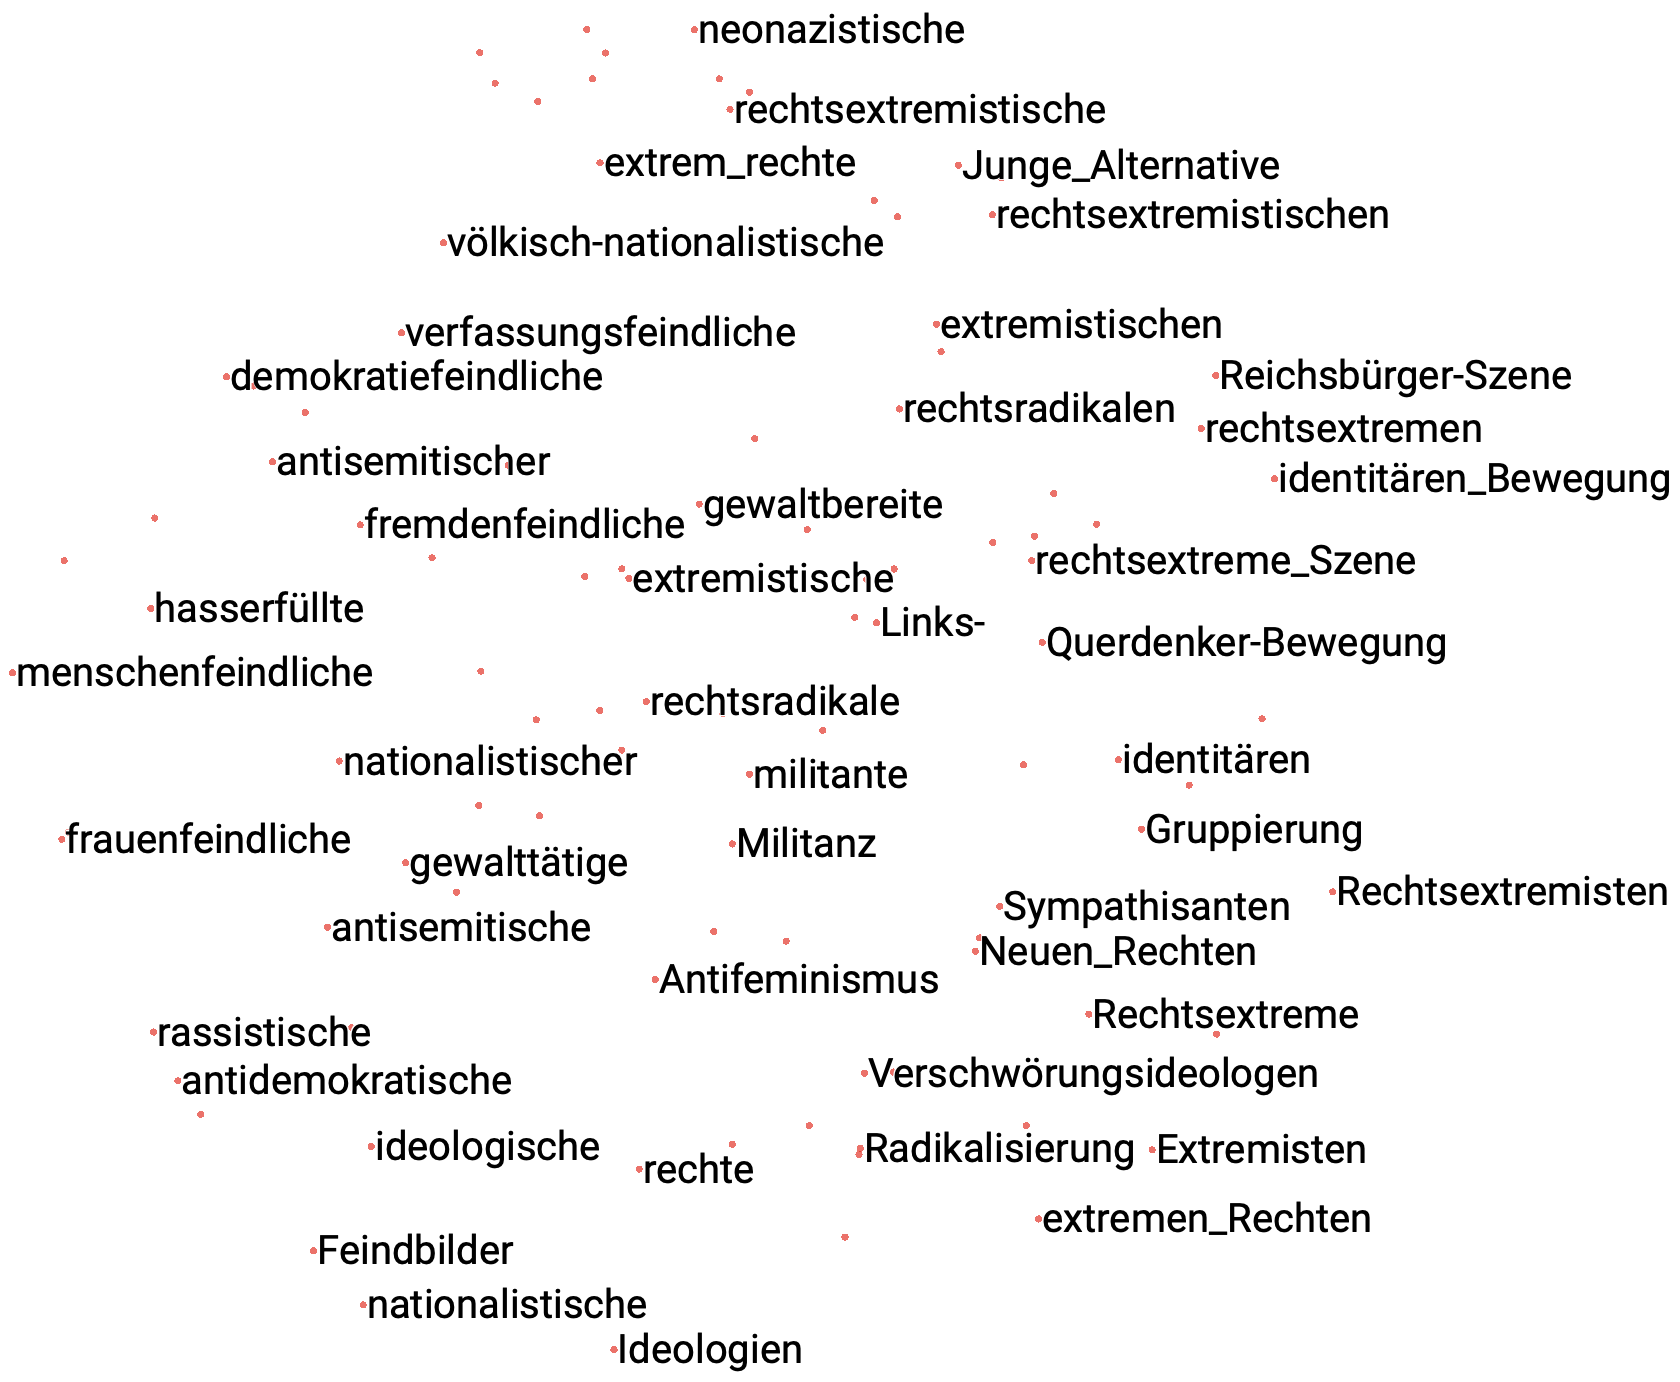
\includegraphics[width=\textwidth]{figures/media/image16.png}
  \caption{\label{fig:pca-nachbarn-extremistische}Nächste paradigmatische Nachbarn zu \emph{extremistische} im Zeitraum 2020--2021 (Dimensionsreduktion mit PCA).}
\end{figure}

Es wird deutlich, dass sich eine Vielzahl semantisch und oft zugleich morphosyntaktisch sehr ähnlicher Wörter im Umfeld des Wortes befinden, wie z.\,B. \emph{neonazistische}, \emph{rechtsradikale} oder \emph{extremistischen}. Andere Ausdrücke erscheinen nicht gleichermaßen bedeutungsähnlich, lassen sich jedoch unschwer als zum Extremismusdiskurs gehörig identifizieren und spielen in diesem etwa als Akteure bzw. Organisationen (u.\,a. \emph{Querdenker-Bewegung}, \emph{Reichsbürger-Szene}, \emph{Neuen\_Rechten}, \emph{Gruppierung}), oder geradezu definitorische Charakteristika (u.\,a. \emph{antidemokratische}, \emph{verfassungsfeindliche}, \emph{ideologische}) eine Rolle. Es deutet sich zudem an, dass es nicht notwendig ist, diese Kategorien im Vorhinein zu definieren und auf die Daten anzuwenden. Vielmehr finden wir sie in der Struktur des Vektorraums bereits wieder und können Cluster erkennen (rechts: Akteure und Organisationen; links: Charakteristika von Extremismus; oben: globalere attributive Bezeichnungen für Extremismus(-formen)). Die Kategorien sind darüber hinaus in diskursanalytischer Literatur bereits als für den Extremismusdiskurs bedeutsam und strategisch veränderlich herausgearbeitet (\chapref{extremismus-in-den-sozialwissenschaften} und \ref{extremismus-diskurs}) und in \chapref{inhaltliche-mindestanforderungen-an-einen-extremismus-frame} als Kandidaten für FE eines Extremismus-Frames ins Auge gefasst worden. Es liegt daher nahe, Cluster von Word Embeddings als FE zu operationalisieren.

Um nicht bei einer visuellen Inspektion einzelner Cluster um ausgewählte Wörter zu verbleiben, ist es sinnvoll, den gesamten Datensatz einem Clustering-Verfahren zu unterziehen. Hierzu wurde der in \chapref{clustering-von-word-embeddings} beschriebene \emph{k-Means}-Algorithmus verwendet, der auch große Datenmengen prozessieren und in eine zuvor festgelegte Anzahl von \emph{k} Clustern gliedern kann. Die Wahl des Parameters ‚\emph{k}` ist dabei natürlich entscheidend und es bestehen unterschiedliche Möglichkeiten, diesen auszuwählen. Mitunter wird von Seiten korpuslinguistischer Diskursanalytiker*innen die Kritik geäußert, dass sich Arbeiten, die solche Verfahren verwenden, zwar einen objektivistischen Anstrich geben wollen, durch die Wahl einzelner Parameter ihre Ergebnisse aber auf eine Art vorformen, die dem \emph{cherry-picking} nahekommt. So formulieren Brookes \& McEnery in Bezug auf die Auswahl von \emph{k} bei Topic Modeling:

\begin{quote}
Total accountability and falsifiability present a way for discourse analysts to avoid the charge of cherry-picking examples to prove a particular argument (Widdowson, 2004). Similarly, topic modelling appears objective and data-driven in as much as the topic discovery procedure is automatic and there seems to be limited scope for the human user to impose any extra-data or pre-analytical categories onto the topics generated. However, as we pointed out earlier in this section, the human researcher is still required to make an important decision about the number of topics generated. This decision is relatively arbitrary. \autocite[7]{brookesUtilityTopicModelling2019}
\end{quote}

Während die Autoren durchaus relevante Probleme am Beispiel der datengeleiteten Generierung von \emph{topics} aufzeigen, die in vielen Beiträgen mehr reflektiert werden müssten, ist ihre Kritik in Bezug auf die Wahl von \emph{k} m.\,E. nicht berechtigt, zumindest wenn die Festlegung gar nicht als ‚objektive` Entscheidung intendiert ist. Vielmehr stellt die Wahl des Parameters eben eine Strukturierungsmöglichkeit der Daten dar, die unterschiedlich fein- oder grobgranulare Ergebnisse zu Tage fördern kann. Ähnlich wie bei einem Mikroskop gilt es also, das methodische Instrument so einzustellen, dass für die jeweilige Forschungsfrage relevante Strukturen sichtbar werden. Dabei kann es auch sinnvoll sein, mit verschiedenen \emph{k} parallel zu arbeiten, wenn es so gelingt, Makro- und Mikrostrukturen herauszuarbeiten und zu kontrastieren. Anstatt den Output eines solchen Verfahrens also als ‚objektiv` anzusehen und zu versuchen, sich der einen ‚richtigen` Variante anzunähern, sollten die Resultate als eine mögliche Strukturierung unter vielen gesehen werden. Auch der Vergleich verschiedener Outputs könnte dann von Interesse sein. Zum Beispiel wäre es denkbar, nachzuverfolgen, welche Wörter bei geringerer Cluster-Größe zusammengefasst und bei höherem \emph{k} voneinander getrennt werden, um lexikalisch-semantische Hierarchien sichtbar zu machen.

In der vorliegenden Arbeit wurde mit unterschiedlichen Cluster-Mengen experimentiert. Beginnend mit einer Einstellung von \emph{k} = 2000, wie sie von Bubenhofer \autocite*{bubenhoferExplorationSemantischerRaeume2022} für Pressedaten verwendet wurde, wurden verschiedene Einstellungen erprobt, wobei sich eine Orientierung an der Korpusgröße bzw. der Anzahl der Vektoren als sinnvoll erwiesen hat. Es erschien also nicht so zu sein, dass das semantische Kategorieninventar von einem Punkt an ausdifferenziert war und zusätzliche Types einfach in diese Kategorien eingeordnet werden. Stattdessen war die Folge einer höheren Type-Anzahl bei gleichbleibendem \emph{k}, dass einzelne Cluster heterogen wurden, also z.\,B. Akteure und ihre Handlungen in den gleichen Clustern zu finden waren. Letztlich wurde entschieden, \emph{k} auf 2,4 \% der Embedding-Anzahl, d.\,h. der Types mit einer Mindestfrequenz von 25 (siehe zu den Type-Anzahlen \chapref{kenndaten-zum-korpus-und-korpusaufbereitung}) einzustellen. So ergaben sich für die diachronen Subkorpora zwischen 2649 (2020--2021) und 4882 (2011--2013) Cluster, für die Zeitungskorpora zwischen 8225 (\textsc{Spiegel}) und 8779 (\textsc{Taz}) Cluster. \tabref{tab:example_clusters} zeigt drei Beispiel-Cluster aus dem Subkorpus 2014--2016, die jeweils nach den drei zentralsten enthaltenen Wortvektoren benannt sind.
\largerpage[-1]
\begin{table}
\caption{Drei Beispiel-Cluster des Zeitraums 2014--2016 und alle enthaltenen Wörter (gereiht nach Nähe zum Cluster-Centroid).}
\label{tab:example_clusters}
 \begin{tabularx}{\textwidth}{>{\hsize=0.5\hsize}X >{\hsize=1.5\hsize}X}
  \lsptoprule
  Cluster & Enthaltene Wörter \\
  \midrule
  \cluster{rechtsradikale{\breakbar}rechtsradikalen{\breakbar}rechtsextreme} & \emph{rechtsradikale, rechtsradikalen, rechtsextreme, rechtspopulistischen, rechtsextremen, rechte, rassistischen, fremdenfeindliche, fremdenfeindlichen, nationalistische, nationalistischen, rechtspopulistische, rechter, antisemitischen, rassistische, antisemitische, rechten, radikalen, radikale, linker, Erstarken} \\
  
  \cluster{Asylbewerber\-unterkunft{\breakbar}Asylunterkunft{\breakbar}Asylbewerberheim} & \emph{Asylbewerberunterkunft, Asylunterkunft, Asylbewerberheim, Gaststätte, Flüchtlingsheim, Lagerhalle, Mehrfamilienhaus, Scheune, Kaserne, Brandstiftung, Synagoge} \\
  
  \cluster{Heidenau{\breakbar}Freital{\breakbar}Bautzen} & \emph{Heidenau, Freital, Bautzen, Clausnitz, Tröglitz, Hoyerswerda} \\
  \lspbottomrule
 \end{tabularx}
\end{table}
Mithilfe des Clusterings gelingt es also, datengeleitet semantische Kategorien, die in der sprachlichen Oberfläche enkodiert und als FE eines Extremismus-Frames lesbar sind, zu erschließen. Hier könnte man die FE als ‚Attribute rechtsextremener Akteure`, ‚Ziele rechter Brandanschläge` und ‚Orte rechtsextremer Anschläge in Ostdeutschland` lesen. Dabei ist die Sichtung der zu einem Cluster gehörigen Wörter und ihre Interpretation als FE ein hermeneutischer Akt. Sein Ziel besteht darin, den größtmöglichen gemeinsamen semantischen Nenner der im Cluster enthaltenen Wörter zu identifizieren. Dabei muss nicht auf das reduktionistische Konzept einer lexikalischen Ausdrucksbedeutung zurückgegriffen werden. Stattdessen können paradigmatische (die anderen Wörter des Clusters) und syntagmatische (kookkurrierende Cluster) Kontextualisierungshinweise einbezogen werden; insbesondere wenn die Interpretation auf Basis des visualisierten Graphen erfolgt. So wird schnell ersichtlich, dass etwa \cluster{14\_Heidenau{\breakbar}Freital{\breakbar}Bautzen} mit anderen Clustern wie u.\,a. \cluster{14\_Notunterkunft{\breakbar}Erstaufnahmeeinrichtung{\breakbar}Unterkunft}, \cluster{14\_Bränden{\breakbar}Unfällen{\breakbar}Zwischenfällen}, \cluster{14\_Ausschreitungen} vorkommt und insofern nicht einfach als ‚Orte` oder ‚Kleinstädte` gelesen werden kann. Es kommt dabei regelmäßig vor, dass sich ein solcher gemeinsamer Nenner für die meisten Wörter finden lässt, jedoch einzelne andere Wörter des Clusters davon mehr oder weniger abweichen. Dies zeigt sich z.\,B. beim Cluster \cluster{14\_rechtsradikale{\breakbar}rechtsradikalen{\breakbar}rechtsextreme}, das auch \emph{linker} und \emph{Erstarken} an seinen Rändern enthält. Auf dieses und andere potenzielle Probleme bei der Auswertung der gewonnenen distributionellen Muster wird in \chapref{wie-der-graph-zu-lesen-ist-und-moegliche-fallstricke} noch vertieft eingegangen.

\subsubsection{Nähe im Vektorraum als Frame-Evokationspotenzial und Perspektivierung}\label{naehe-im-vektorraum-als-frame-evokationspotenzial-und-perspektivierung}

Auf Basis des geclusterten WEM ist es nun möglich, nicht nur die benachbarten Wörter, sondern auch benachbarte Cluster zu Wörtern oder anderen Clustern zu berechnen. Jedes Cluster wird dabei durch den Vektor repräsentiert, der den Mittelpunkt des Clusters, d.\,h. mathematisch das arithmetische Mittel der beinhalteten Vektoren, darstellt. So ist das Embedding \emph{Npd} in der \textsc{Welt} umgeben von den Clustern \cluster{we\_Rechtsextremisten{\breakbar}Neonazis{\breakbar}Rechtsextremen}, \cluster{we\_Linkspartei{\breakbar}Pds{\breakbar}Linken}, \cluster{we\_Gauland{\breakbar}Meuthen{\breakbar}Petry}, \cluster{we\_Verfassungsschutz} und \cluster{we\_rechtsradikalen{\breakbar}rechtsextremistischen{\breakbar}linksextremen}. Es wird deutlich, dass auf diese Weise ein breiter Teil des verstehensrelevanten Wissens zu einzelnen Wörtern zugänglich ist. Frame-semantisch gewendet lassen sich die benachbarten Cluster als FE eines durch das abgefragte Wort evozierten Frames interpretieren, etwa als rechte parlamentarische (\cluster{we\_Gauland{\breakbar}Meuthen{\breakbar}Petry}) und außerparlamentarische (\cluster{we\_Rechtsextremisten{\breakbar}Neonazis{\breakbar}Rechtsextremen}) Akteure, institutionelle Gegenspieler (\cluster{we\_Verfassungsschutz}) oder attributive Zuschreibungen (\cluster{we\_rechtsradikalen{\breakbar}rechtsextremistischen{\breakbar}linksextremen}).

Um die Cluster zu identifizieren, die eine Rolle im Extremismusdiskurs spielen, wurde ein Verfahren entwickelt, das in der Lage ist, anhand einiger weniger \emph{seed words} jedes Cluster in Hinblick auf seine semantische Nähe zum Extremismusdiskurs zu verorten. Die einzelnen ausgewählten \emph{seed words} spielen dabei eine untergeordnete Rolle, da sie nur den Ausgangspunkt für ein Verfahren darstellen, das ein sehr breites lexikalisches Repertoire an thematisch einschlägigen Wörtern und mithin Möglichkeiten des Framings zu Tage fördert. Die Auswahl der \emph{seed words} sollte einerseits auf Basis der FE eines losen provisorischen Frame-Konzeptes, wie es in \chapref{inhaltliche-mindestanforderungen-an-einen-extremismus-frame} skizziert wurde, andererseits auf Basis morphosyntaktischer Kategorien erfolgen, da das Word-Embedding-Modell sowohl auf semantischen als auch auf grammatischen Faktoren beruht. Auf Basis der \emph{seed words}\footnote{Es wurden die folgenden \emph{seed words} verwendet: \emph{Extremismus}, \emph{extremistische}, \emph{extremistisch}, \emph{Radikalismus}, \emph{Rechtsextremismus}, \emph{rechtsextremistische}, \emph{rechtsextremistisch}, \emph{rechtsradikale}, \emph{rechtsradikal}, \emph{Rechtsradikalismus}, \emph{Linksextremismus}, \emph{linksextremistische}, \emph{linksextremistisch}, \emph{linksradikale}, \emph{linksradikal}, \emph{Linksradikalismus}, \emph{Islamismus}, \emph{islamistische}, \emph{islamistisch}, \emph{angreifen}, \emph{begangen}, \emph{verübt}, \emph{Attentat}, \emph{Anschlag}, \emph{Npd}, \emph{Neonazis}, \emph{Antifa}, \emph{islamischer}\cluster{\_}\emph{Staat}, \emph{Bin}\cluster{\_}\emph{Laden}, \emph{Taliban}.}, die einerseits die etablierten Extremismusvarianten ‚Rechtsextremismus`, ‚Linksextremismus` und ‚Islamismus`, andererseits unterschiedliche Flexionsformen und Wortarten abdecken, konnte eine Liste von Clustern berechnet werden, die eine thematische Nähe zum Extremismusdiskurs aufweisen, d.\,h. FE in einem Extremismus-Frame darstellen. Die genauere Funktionsweise des Verfahrens wird in \chapref{berechnung-des-extremismus-centroid-und-begrenzung-der-knotenmenge} dargestellt. Der Mittelpunkt dieser berechneten Cluster, im Folgenden als Extremismus-Centroid bezeichnet, kann nun als Referenzpunkt dienen, um andere Punkte im Vektorraum wie einzelne Word-Embeddings oder Cluster-Centroids hinsichtlich ihrer semantischen Nähe zum Thema Extremismus zu verorten. \tabref{tab:cluster_distances_centroid} zeigt ausschnittsweise die Ergebnisse dieser Analyse für die \textsc{Taz}. Es wird deutlich, dass die Cluster, die dem Extremismus-Centroid relativ nah sind, in der Tat Wörter enthalten, die eindeutig Teil des Extremismusdiskurses sind bzw. einen Extremismus-Frame evozieren (z.\,B. \emph{Extremisten}, \emph{Hisbollah}, \emph{Neonazis}), während die positiv konnotierten Wörter am anderen Ende des Spektrums wie \emph{schwärmt} oder \emph{tolle} keinen Bezug zum Thema Extremismus aufweisen.

\begin{table}[b]
\caption{Beispiele für Cluster mit unterschiedlicher Distanz zum Extremismus-Centroid.}
\label{tab:cluster_distances_centroid}
 \begin{tabularx}{\textwidth}{>{\hsize=0.6\hsize}X >{\hsize=1.4\hsize}X}
  \lsptoprule
  Cosinus-Ähnlichkeit & Cluster \\
  \midrule
  sehr hoch (\textgreater= 0.53) & \cluster{ta\_Extremisten{\breakbar}Islamisten{\breakbar}Dschihadisten} (0.78) \\
                                & \cluster{ta\_Hisbollah{\breakbar}Hamas{\breakbar}Pkk} (0.73) \\
                                & \cluster{ta\_Terrorismus{\breakbar}Terror} (0.65) \\
                                & \cluster{ta\_Rechtsextremisten{\breakbar}Neonazis{\breakbar}Rechtsextremen} (0.53) \\
  \midrule
  eher hoch (\textasciitilde{} 0.27) & \cluster{ta\_Rede} (0.27) \\
                                     & \cluster{ta\_Verbreitung} (0.27) \\
                                     & \cluster{ta\_Unterschrift} (0.27) \\
                                     & \cluster{ta\_Rot-grün{\breakbar}Schwarz-gelb} (0.27) \\
  \midrule
  eher niedrig (\textasciitilde{} 0.14) & \cluster{ta\_Krankenkassen{\breakbar}Kassen} (0.14) \\
                                        & \cluster{ta\_Privatisierung} (0.14) \\
                                        & \cluster{ta\_Plänen} (0.14) \\
                                        & \cluster{ta\_Sachbearbeiterin{\breakbar}Sekretärin{\breakbar}Putzfrau} (0.14) \\
  \midrule
  sehr niedrig (\textless= -0.31) & \cluster{ta\_samt{\breakbar}nebst{\breakbar}inklusive} (-0.31) \\
                                  & \cluster{ta\_bietet} (-0.31) \\
                                  & \cluster{ta\_wunderbare{\breakbar}tolle{\breakbar}schöne} (-0.39) \\
                                  & \cluster{ta\_schwärmt} (-0.39) \\
  \lspbottomrule
 \end{tabularx}
\end{table}
Dass Cluster, die die ausgewählten \emph{seed words} beinhalten, besonders nah am Extremismus-Centroid zu finden sind, liegt in der gewählten Methodik begründet, da sie ja der Ausgangspunkt für dessen Berechnung sind. Unter den 1256 Clustern mit insgesamt 70\,393 Types, die im \textsc{Taz}-Frame einbezogen wurden, enthalten jedoch nur 21 Cluster \emph{seed words}, sodass die Methode es hier durchaus erlaubt, weit über diese hinauszugehen. Dies zeigen auch die Cluster in der Tabelle mit einer eher hohen Cosinus-Ähnlichkeit. Sie können als Teil des politischen Vokabulars durchaus eine Rolle im Extremismusdiskurs spielen, sind aber auch Teil einer Vielzahl anderer thematischer Diskurse. Die Wörter mit einer eher niedrigen Cosinus-Ähnlichkeit wiederum haben zumindest noch entfernt mit dem politisch-institutionellen Bereich zu tun, während die Wörter am unteren Ende der Skala wohl nur sehr selten im Extremismusdiskurs vorkommen. Insgesamt ist bei der Analyse jedoch zu beachten, dass sie eher eine grobe Orientierung bietet und man einzelne Cluster von Hand wahrscheinlich anders ordnen würde. Sie ermöglicht unter Frame-semantischer Perspektive jedoch näherungsweise, das Evokationspotenzial von Wörtern als Spektrum zu modellieren. Dies ist kongruent mit Barsalous und Minskys Annahme eines probabilistischen „matching process`` \autocite*[2]{minskyFrameworkRepresentingKnowledge1974} beim Aufrufen von Frames und geht über \emph{FrameNet} hinaus, wo einzelne LE einem Frame gleichberechtigt zugeordnet sind. Wollte man die Fillmore'sche Trennung von \emph{evocation} und \emph{invocation} aufrechterhalten \autocite[dazu kritisch][]{busseFrameSemantikKompendium2012} und diese zugleich (distributionell\mbox{-}) semantisch statt valenzgrammatisch begründen, könnte man sie anhand der sortierten Cluster-Liste vornehmen, indem man einen Cosinus-Wert als Grenzwert festlegt. Man müsste sich aber im Klaren sein, dass man es dabei mit der notwendigerweise vereinfachenden Einteilung eines Spektrums in zwei Kategorien zu tun hat, nicht mit einem genuin binären linguistischen Phänomen.

Durch die datengeleitete Einteilung des Korpus in Wort-Cluster, die mehr oder weniger Teil des Extremismusdiskurses sind, und ihre Operationalisierung als FE, eröffnet sich zudem eine erste Möglichkeit, Perspektivierung als einen Grundbestandteil Frame-semantischer Theorien (siehe \chapref{perspektivierung-kontext-und-frame-wandel}) abzubilden. Bezieht man nämlich bei der Rekonstruktion des Extremismus-Frames nur die Cluster ein, die eine gewisse Nähe zum Extremismus-Centroid aufweisen, werden kontextfremde Relationen polysemer Cluster ausgeblendet (siehe zur Operationalisierung der FE-Relationen Kapitel \ref{kollokation-von-word-embedding-clustern-als-frame-relationen-und-perspektivierung-kollokationsnetzwerke-als-frames}). Zu einem Cluster wie \cluster{17\_Lastwagen{\breakbar}Lkw} werden also nicht alle syntagmatisch assoziierten FE wie u.\,a. auch \cluster{17\_Fahrzeuge{\breakbar}Autos{\breakbar}Pkw} oder \cluster{17\_beim\_Überholen{\breakbar}am\_Fahrbahnrand{\breakbar}Müllwagen} dargestellt, sondern insbesondere solche, die für den Extremismus-Diskurs thematisch einschlägig sind und es so in Hinblick auf seine Semantik im Extremismusdiskurs bzw. im Kontext des Anschlags vom Berliner Breitscheid-Platz perspektivieren (\cluster{17\_Attentäter}, \cluster{17\_Amri}, \cluster{17\_getötet\_worden{\breakbar}verletzt\_worden{\breakbar}ums\_Leben\_gekommen}).

Betrachtet man noch einmal die in den Word-Embedding-Clustern enthaltenen Wörter (\tabref{tab:example_clusters}) und paradigmatische Cluster-Nachbarschaften (siehe \tabref{tab:collocations_neighbors} im folgenden Kapitel), so wird die paradigmatische Ausrichtung von WEM deutlich. In einem Cluster wie \cluster{14\_Heidenau{\breakbar}Freital{\breakbar}Bautzen} finden sich ausschließlich andere Kleinstädte, jedoch keine Ausdrücke wie \emph{leben}, \emph{ostdeutsch}, \emph{protestieren} oder \emph{Brandanschlag}, die man im syntagmatischen Umfeld erwarten könnte. Um Frame-semantische Relationen zwischen den Clustern beschreiben zu können, wurde daher ihre Distribution auf der syntagmatischen Achse, d.\,h. Kollokationen der Cluster miteinander, berechnet. Das folgende Kapitel wird zeigen, wie sich diese Kollokationen als Frame-Relationen lesen lassen.

\subsubsection{Kollokation von Word-Embedding-Clustern als Frame-Relationen und Perspektivierung, Kollokationsnetzwerke als Frames}\label{kollokation-von-word-embedding-clustern-als-frame-relationen-und-perspektivierung-kollokationsnetzwerke-als-frames}

Die Kollokation, d.\,h. das statistisch signifikante gemeinsame Auftreten von Wörtern \autocite{bubenhoferSprachgebrauchsmusterKorpuslinguistikAls2009}, ist eines der zentralen Konzepte in korpuslinguistischen Ansätzen (siehe \chapref{distributionelle-semantik}, \ref{distributionell-semantische-methodik} und \ref{kollokationen-als-syntagmatische-distributionelle-muster}). Kollokationen beschreiben sprachoberflächliche Distributionen von Korpus-Types (typischerweise Wortformen oder Lemmata) auf der syntagmatischen Achse. Sie machen also die Interaktion von Wörtern sichtbar, jedoch ohne dabei etwas über den Typ der Interaktion auszusagen, also z.\,B. in welchem grammatischen oder semantischen Verhältnis sie stehen. Während die Berechnung von Kollokationen klassischerweise zu den \emph{corpus-based} Methoden zählt, ist die Berechnung ganzer Kollokationsnetze, bei der für jeden Korpus-Type seine Kollokatoren berechnet werden, ein \emph{corpus-driven} Verfahren, das nicht nur auf ausgewählte Wörter angewandt wird (siehe \chapref{begriffsklaerungen-quantitativ-und-qualitativ-corpus-driven-und-corpus-based-sowie-die-rolle-von-hermeneutik}). Hinsichtlich des Ansinnens dieser Arbeit, eine induktive Beschreibung von Extremismus-Frames zu leisten, erscheinen Kollokationsnetze daher geeignet. Ihre Berechnung für ganze Korpora kann jedoch -- je nach Korpusgröße -- sehr rechenintensiv sein und der Output der Analyse aufgrund der Vielzahl der berechneten Kollokationsbeziehungen kaum interpretierbar.\footnote{Für die Subkorpora würden sich Matrizen mit bis zu 365815 x 365815 Werten ergeben (siehe Type-Anzahlen in \tabref{tab:type_frequencies} in \chapref{kenndaten-zum-korpus-und-korpusaufbereitung}).} Für den Einsatz von Kollokationsnetzen ist es also notwendig, die Anzahl der einbezogenen Types mithilfe eines transparenten und begründeten Verfahrens zu reduzieren. So kann man entweder nur lokale Anteile von Kollokationsnetzen um einzelne Wörter betrachten, was wiederum einer verengten \emph{corpus-based} Perspektive entspricht, oder die Type-Anzahl insgesamt reduzieren. Für die Rekonstruktion von Frames, die ich hier in Form eines Kollokationsnetzes anstrebe, sind wesentliche Schritte einer solchen Reduktion durch die im vorigen Kapitel gemachten Ausführungen bereits geleistet. Zum einen werden die Wort-Types des Korpus durch das Clustering auf eine um ein Vielfaches geringere Anzahl von Cluster-Types reduziert. Zum anderen können durch die Berechnung des Evokationspotenzials der einzelnen Cluster solche Cluster aus der Analyse ausgeschlossen werden, die nur mit einer geringen Wahrscheinlichkeit einen Extremismus-Frame evozieren.

\begin{table}\small
\caption{Kollokationen und \emph{next neighbours} im Word-Embedding-Modell zum Cluster \cluster{11\_festgenommen}.}
\label{tab:collocations_neighbors}
 \begin{tabularx}{\textwidth}{lXrXr}
  \lsptoprule
  Rang & Syntagmatisch benachbarte Cluster & Log-Likelihood & Paradigmatisch benachbarte Cluster & Cosinus-Ähnlichkeit \\
  \midrule
  1  & \cluster{11\_wurden}                              & 9420.50   & \cluster{11\_festgenommen\_worden}                     & 0.82 \\
  2  & \cluster{11\_wurde}                               & 8247.68   & \cluster{11\_getötet{\breakbar}erschossen}               & 0.76 \\
  3  & \cluster{11\_Polizei}                             & 4277.99   & \cluster{11\_inhaftiert{\breakbar}hingerichtet{\breakbar}gefoltert} & 0.72 \\
  4  & \cluster{11\_Verdächtigen{\breakbar}Tatverdächtigen{\breakbar}mutmaßlichen\_Täter} & 1983.41 & \cluster{11\_beschuldigt{\breakbar}verdächtigt{\breakbar}angeklagt} & 0.70 \\
  5  & \cluster{11\_Personen}                            & 1749.90   & \cluster{11\_geschnappt{\breakbar}verhört{\breakbar}vernommen} & 0.69 \\
  6  & \cluster{11\_sieben{\breakbar}sechs{\breakbar}fünf}   & 1741.97   & \cluster{11\_ermordet{\breakbar}umgebracht{\breakbar}entführt} & 0.69 \\
  7  & \cluster{11\_Hund{\breakbar}Mann{\breakbar}Tier}      & 1333.86   & \cluster{11\_Entführung{\breakbar}Tötung{\breakbar}Ermordung} & 0.61 \\
  8  & \cluster{11\_31-Jähriger{\breakbar}27-Jähriger{\breakbar}44-Jähriger} & 1130.97 & \cluster{11\_Durchsuchungen{\breakbar}Razzia{\breakbar}Razzien} & 0.59 \\
  9  & \cluster{11\_Demonstranten}                      & 1034.54   & \cluster{11\_angegriffen{\breakbar}attackiert}            & 0.59 \\
  10 & \cluster{11\_festgenommen}                       & 1017.76   & \cluster{11\_Verdächtigen{\breakbar}Tatverdächtigen{\breakbar}mutmaßlichen\_Täter} & 0.58 \\
  \lspbottomrule
 \end{tabularx}
\end{table}
Ich habe also ein Kollokationsnetzwerk für alle Word-Embedding-Cluster berechnet. \tabref{tab:collocations_neighbors} bildet jeweils die Top 10 Kollokate und \emph{next neighbours} im Word-Embedding-Modell zum Cluster \cluster{11\_festgenommen} ab. Im Vergleich zeigt sich deutlich, dass der vektorraumbasierten Rangfolge paradigmatische Ähnlichkeit zugrunde liegt. So finden sich in erster Linie andere Verben in der gleichen Flexionsform (Ränge 1--6 sowie 9) oder verbale Konzepte (Ränge 7--8). Erst auf Rang 10 findet sich ein Cluster, das in einem eher syntagmatischen Zusammenhang zum Ausgangscluster steht, nämlich mögliche Patiens zum Verb \emph{festnehmen}. Als Frame-Relationen gelesen kann eine solche paradigmatische Auswertung also Auskunft über ‚prototypisch assoziierte benachbarte (kontige) Konzepte` \autocite{busseFrameSemantikKompendium2012} geben, nicht jedoch über Frame-Relationen, wie sie etwa in den für die Analyse eines verbalen Konzeptes geeigneten Fillmore-Frames angelegt sind. Ganz anders stellt sich die kollokationsbasierte Rangfolge dar. Hier zeigen sich syntagmatische Beziehungen, die sich als Interaktion der Frame-Elemente lesen lassen. So finden sich sowohl mögliche Besetzungen der Agens- (Rang 3) und Patiens-Rolle (Ränge 4--5, 7--9) als auch zusätzliche Möglichkeiten der semantischen Spezifizierung via Attribuierung (Ränge 6 und 8). Die Benennung der Art der Relation zwischen den Frame-Elementen ist dabei ein rein hermeneutischer und mitunter auf umfangreichem Diskurswissen fußender Akt und nicht unmittelbar aus den quantitativen Daten ablesbar (siehe dazu ausführlicher \chapref{begriffsklaerungen-quantitativ-und-qualitativ-corpus-driven-und-corpus-based-sowie-die-rolle-von-hermeneutik}). Die Kollokationen zeigen also zunächst nur an, dass es einen inhaltlichen Zusammenhang gibt, nicht worin dieser besteht.

Kollokationsnetze bieten neben ihrer induktiven Berechenbarkeit auch den Vorteil, als Netzwerkgraphen visualisierbar zu sein \autocite[siehe ausführlich zu Netzwerkgraphen in der Linguistik][179-192]{bubenhoferVisuelleLinguistikZur2020}. Dabei wurden unter allen Clustern mit einer Mindest-Cosinus-Ähnlichkeit (\textgreater= 0,2 für die diachronen, \textgreater= 0,24 für die Zeitungskorpora) zum Extremismus-Centroid des Zeitraumes jeweils die 20 Cluster mit dem höchsten Kollokationsscore zu diesem Cluster einbezogen. Die Cluster fungieren sodann als Knoten des Graphen, während die Kollokationsscores die Kanten darstellen. Die folgenden Abbildungen zeigen den vollständigen Graphen für die Jahre 2020--2021 (\figref{fig:extremismus-frame-2020-21}), einen Ausschnitt dieses Graphen, in dem Wort-Cluster des Themenfeldes ‚Politik` enthalten sind (\figref{fig:politik-frame-2020-21}), sowie das Cluster \cluster{20\_Hanau} und seine Verbindungen im Graphen (\figref{fig:hanau-frame-2020-21}). Besser explorierbar ist das Netzwerk in der interaktiven Browser-Ansicht; Hinweise zur Bedienung finden sich in \chapref{ueberblick-und-bedienung}. Die erzeugten Visualisierungen sind unter \url{https://doi.org/10.5281/zenodo.10888812} veröffentlicht.

\begin{figure}[t]
  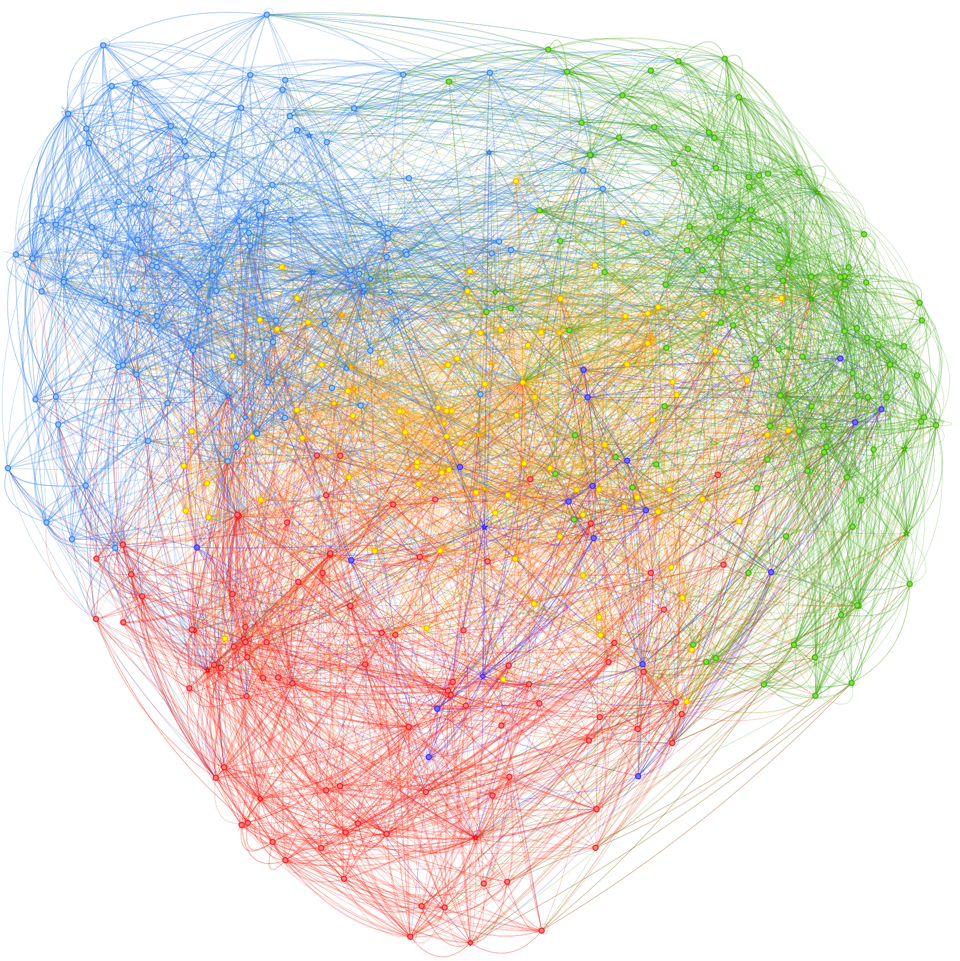
\includegraphics[width=\textwidth]{figures/media/image18.png}
  \caption{\label{fig:extremismus-frame-2020-21}Extremismus-Frame des Zeitraumes 2020--2021.}
\end{figure}

\begin{figure}
  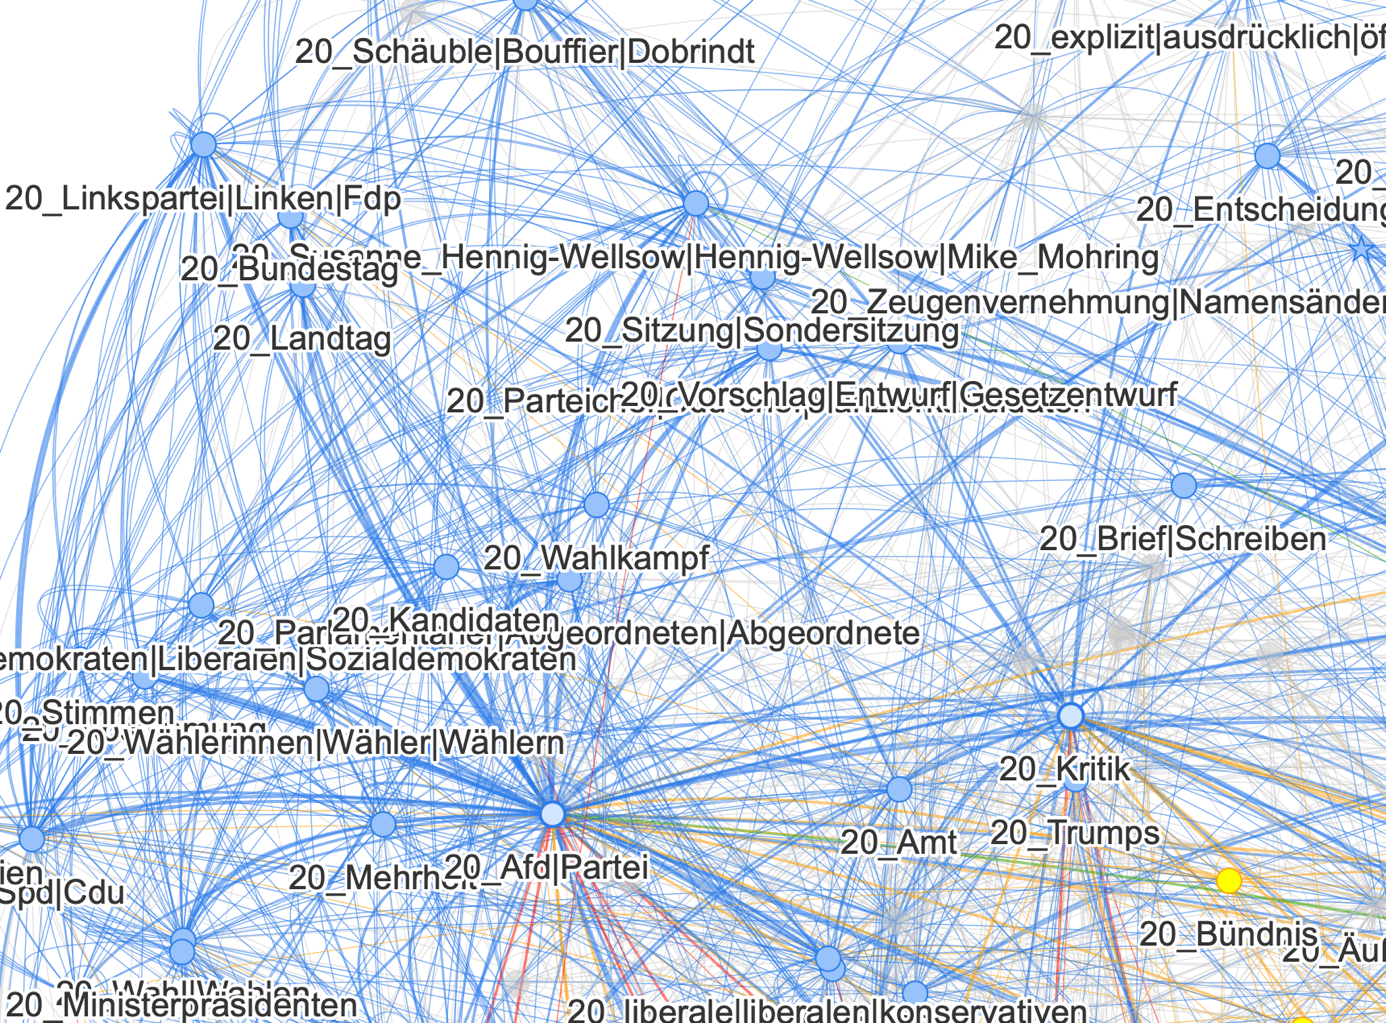
\includegraphics[width=\textwidth]{figures/media/image17.png}
  \caption{\label{fig:politik-frame-2020-21}Ausschnitt aus dem Politik-Teil-Frame des Zeitraums 2020--2021.}
\end{figure}

\begin{figure}
  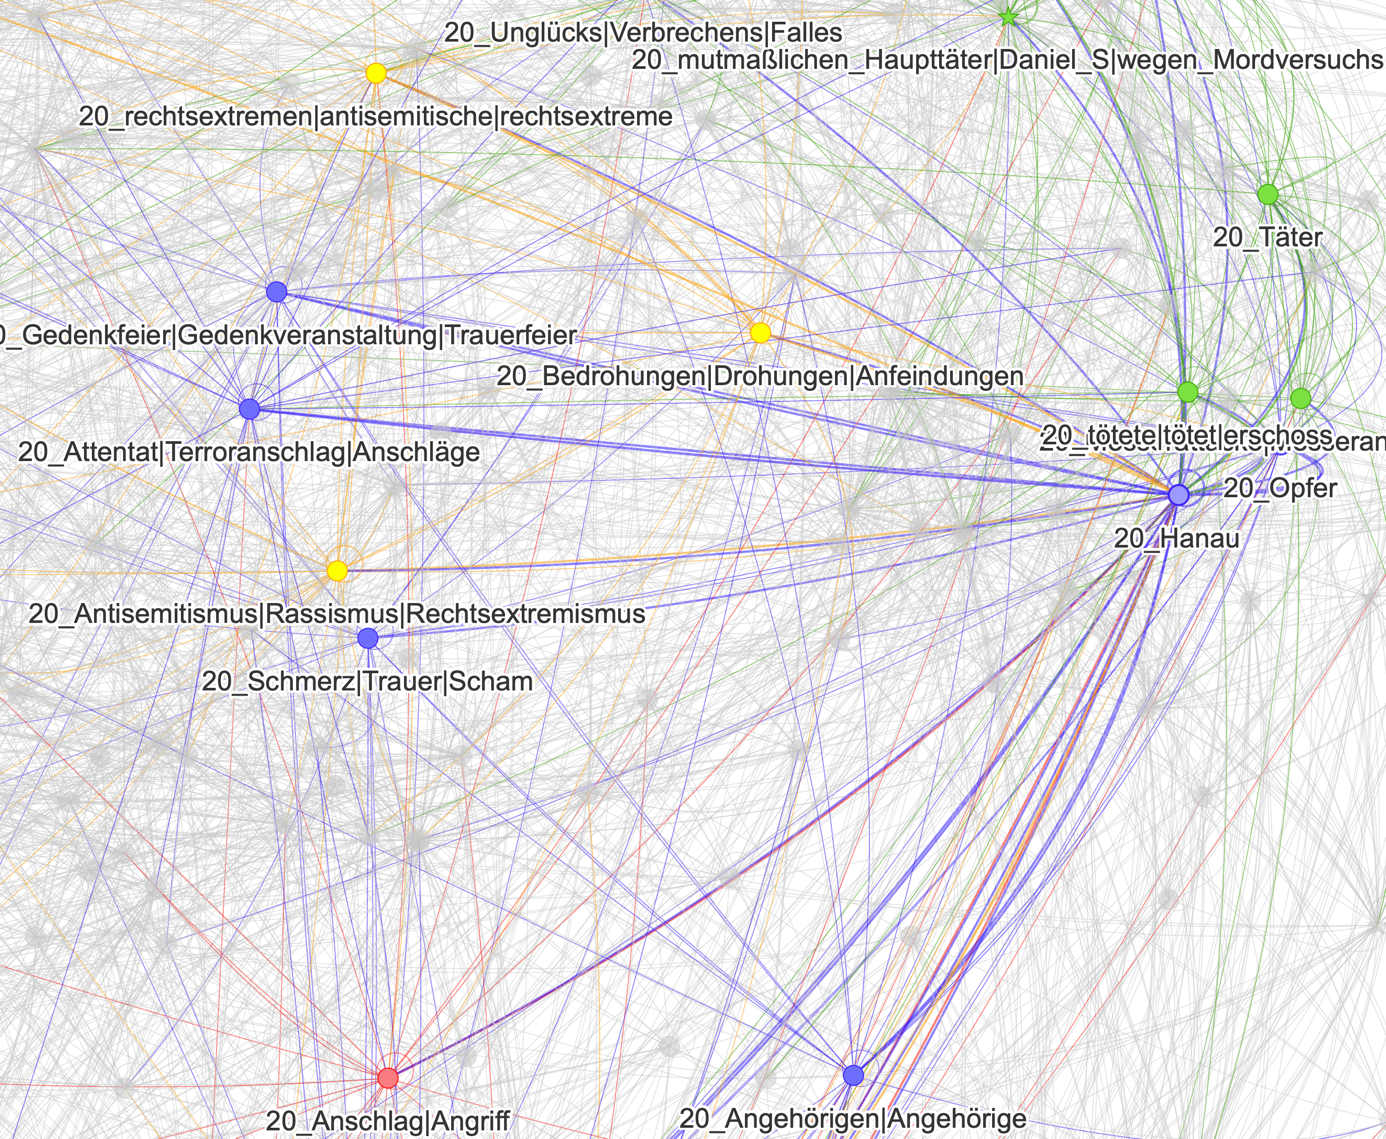
\includegraphics[width=\textwidth]{figures/media/image19.png}
  \caption{\label{fig:hanau-frame-2020-21}Teil des Hanau-Frame des Zeitraums 2020--2021.}
\end{figure}

Das so erstellte Netzwerk kann nun als (Type\mbox{-})Frame gelesen werden, der wesentliche Merkmale von Busse-Frames modelliert. Insbesondere sind dies die Slot-Filler-Struktur, die Rekursivität und unterschiedliche Arten der Frame-Relationen. Die Slot-Filler-Struktur und das Merkmal der Rekursivität sind dabei eng zusammen zu denken: Es lässt sich sowohl das gesamte Netzwerk als ein Frame lesen, der sich aus verschiedenen FE (Slots) zusammensetzt; auch an diese sind jedoch andere FE als Filler angeschlossen, die in Bezug auf wiederum andere FE als Slots agieren. Die Konstituenten der FE, also einzelne zu einem Cluster zusammengefasste Wörter, stellen zugleich die LE dar, die dieses FE evozieren, und darüber hinaus potenzielle Filler eines durch die Liste der LE definierten Wertebereichs. Beispielsweise ist an das Cluster \cluster{20\_Afd{\breakbar}Partei} das Cluster \cluster{20\_Höcke{\breakbar}Kalbitz{\breakbar}Andreas\_Kalbitz} angeschlossen, das im Sinne eines FE ‚Akteure der AfD` interpretierbar ist. Die einzelnen enthaltenen Wörter wie \emph{Kalbitz}, \emph{Flügel} oder \emph{Meuthen} stellen Mögliche Instantiierungen des FE in Token-Frames dar. Dieses FE ist nun selbst wieder ein komplexer Frame und angeschlossene Cluster wie \cluster{20\_Verfassungsschutz}, \cluster{20\_Einstufung} oder \cluster{20\_rechtsradikalen{\breakbar}rechtsradikale{\breakbar}rechtsextremistischen} zeigen an, dass in diesem Zeitraum insbesondere der \emph{Flügel} um \emph{Björn\_Höcke} unter Extremismusverdacht steht bzw. als rechtsextremistisch eingestuft wurde.

Die in den obigen Abbildungen gezeigten Ausschnitte des Graphen sind also jeweils als Frames interpretierbar. Der gesamte Graph in \figref{fig:extremismus-frame-2020-21} ist der Extremismus-Frame für den Zeitraum 2020--2021. Er ist unterteilt in fünf thematische Teil-Frames, die strukturell besonders eng zusammenhängen und farblich markiert sind (siehe \chapref{visualisierung-als-netzwerk-graph-und-erkennung-von-communities}). \figref{fig:hanau-frame-2020-21} stellt die Verbindungen des Clusters \cluster{20\_Hanau} im Graphen dar und lässt sich als Frame zum Anschlag in Hanau im Februar 2020 interpretieren. Während diese drei Struktureinheiten des Netzwerks in einem induktiven Zugang bzw. unter Nutzung etablierter Algorithmen emergent werden, ist es auch möglich, vorwissens- bzw. theoriegeleitete Interessen an den Graphen heranzutragen. So können in einem nächsten Schritt Extremismusvarianten-Frames herausgearbeitet werden. Eine grobe Einteilung kristallisiert sich bereits in der datengeleitet ermittelten Netzwerk-Struktur heraus; Islamismus und politischer Extremismus sind hier stets in unterschiedlichen thematischen Teilen des Netzwerks (Krieg \& Islamismus, Demonstrationen \& Politischer Extremismus) zu finden (siehe zur Analyse der Netzwerk-Communities \chapref{makrostruktur-thematische-teil-frames}). Da sich die Varianten-Frames jedoch auch aus anderen thematischen Bereichen speisen, wurden ergänzend weitere Cluster selektiert, die qua ihrer Kernbedeutung, ihrer Nähe zum Extremismus-Centroid oder aufgrund ergänzender \emph{corpus-driven} Analysen (siehe \chapref{vorgehen-und-zielsetzung}) der jeweiligen Extremismus-Variante zugehörig erscheinen. Idealiter ergeben sich Teile dieser Frames bereits aus den deduktiv ermittelten Strukturen und alle Knoten haben mindestens eine Kante zu einem anderen Knoten des Frames.

\begin{figure}[t]
  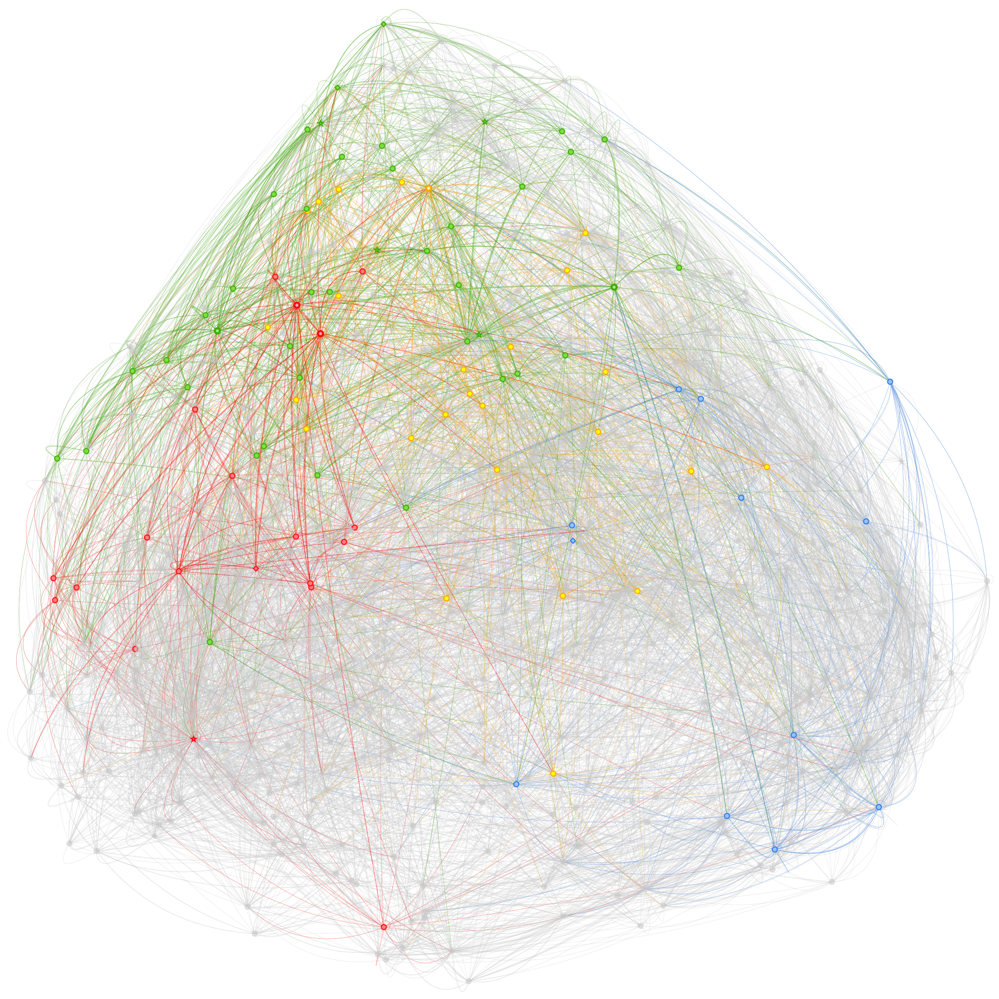
\includegraphics[width=\textwidth]{figures/media/image20.png}
  \caption{\label{fig:rechtsextremismus-frame-1999-2001}Rechtsextremismus-Frame des Zeitraums 1999--2001.}
\end{figure}

~\figref{fig:rechtsextremismus-frame-1999-2001} zeigt die Makrostruktur der Rechtsextremismus-Frames des Zeitraums 1999--2001. Zur Modellierung wurden alle Knoten ausgewählt, die auf Basis von Vorwissen relativ eindeutig der Extremismusvariante zuzuordnen sind (z.\,B. \cluster{99\_Npd}, \cluster{99\_Neonazis{\breakbar}Skinheads{\breakbar}Rechtsextremisten}, siehe \chapref{rechts--und-linksextremismus}). Dieser \emph{corpus-based} Verfahrensschritt ist jedoch eingebettet in die \emph{corpus-driven} ermittelte Struktur, die ergänzend und kontextualisierend wirkt. So werden auch die an die selektierten Knoten angeschlossenen Knoten sowie die Labels der an diese angeschlossenen Knoten angezeigt. Eine Leitlinie besteht außerdem darin, nur solche Knoten auszuwählen, die untereinander vernetzt sind. Dass jeweils ein großer Teil der Knoten zur selben Community gehört, stützt die Hypothese, dass die Extremismusvariante sich auch in der distributionellen Struktur des Korpus niederschlägt. Es finden sich so etwa Praktiken (z.\,B. \cluster{99\_vergewaltigt{\breakbar}überfallen{\breakbar}angegriffen}, \cluster{99\_verletzt\_worden}) und Maßnahmen der Bekämpfung (z.\,B. \cluster{99\_Verbot}, \cluster{99\_verhindern}) als eng assoziiert mit Rechtsextremismus, die nicht vorgegeben waren. Natürlich ist es nicht ausgeschlossen, deduktiv begründete Frames anzunehmen, wenn diese nicht durch die induktiv ermittelte Struktur gedeckt sind. Ausgehend von diesem Ergebnis sollte letztere jedoch noch nicht verworfen werden, sondern geprüft werden, wie der Befund zustande kommen kann -- warum man also einen konzeptuellen Zusammenhang annimmt, der sprachoberflächlich scheinbar nicht realisiert wird. Solche Irritationsmomente können den Blick einerseits auf methodische Defizite lenken, ihn andererseits aber auch für unerwartete Arten der sprachlichen Realisierung von Wissenselementen schärfen und so ein spannender Ausgangspunkt für Folgefragen im Sinne einer ‚quantitativ informierten qualitativen Diskursanalyse` \autocite{bubenhoferQuantitativInformierteQualitative2013} sein.

Die Betrachtung einzelner Knoten des Graphen und ihrer Kanten macht außerdem deutlich, wie einzelne Wörter Frames perspektivieren können. Als Beispiel können die Knoten \cluster{99\_Nazis} und \cluster{99\_Neonazis{\breakbar}Skinheads{\breakbar}Rechtsextremisten} dienen. Beide beinhalten Akteure eines Rechtsextremismus-Frames, die den Frame jedoch jeweils deutlich anders perspektivieren. So ist das Cluster \cluster{99\_Nazis} eng mit dem Bereich des zweiten Weltkriegs bzw. Nationalsozialismus verbunden (u.\,a. \cluster{99\_Holocaust{\breakbar}Nationalsozialismus}, \cluster{99\_Krieg}, \cluster{99\_1945{\breakbar}Zweiten\_Weltkrieg}), während \cluster{99\_Neonazis{\breakbar}Skinheads{\breakbar}Rechtsextremisten} insbesondere in Verbindung mit körperlichen Straftaten und Demonstrationen (u.\,a. \cluster{99\_Demonstranten{\breakbar}Proteste{\breakbar}Protesten}, \cluster{99\_verletzt\_worden}, \cluster{99\_vergewaltigt{\breakbar}überfallen{\breakbar}angegriffen}) vorkommt. Dass sich dies jedoch in einzelnen Vorkommen anders darstellen kann, zeigt Konkordanz K01 in \tabref{tab:K01}.\footnote{Die Konkordanzen werden hier und im Folgenden so wiedergegeben, wie sie im Korpus enthalten sind. Aus diesem Grund ist die Groß- bzw- Kleinschreibung einzelner Wörter verändert und es fehlen Interpunktionszeichen sowie sehr niedrigfrequente Wörter (siehe \chapref{kenndaten-zum-korpus-und-korpusaufbereitung} und \ref{details-der-korpusaufbereitung} zur Korpusaufbereitung).}

\begin{table}
  \caption{Konkordanz zum Ausdruck \emph{Nazis}.}
  \label{tab:K01}
K01 taz\_2208663
\begin{tabularx}{\textwidth}{XcY}
\toprule
man den Rechten keine Plattform geben darf in den Stuben der Verfassungsschutzämter wird lieber geschreddert & \textbf{Nazis} & sind Soziopathen wer sich ihnen offen entgegenstellt braucht Mut und verdient jede Unterstützung ganz am \\
\bottomrule
\end{tabularx}
\end{table}


Man kann diese Äußerung also als Bruch mit dem üblichen Gebrauch des Wortes \emph{Nazis} bzw. der üblichen Versprachlichung zeitgenössischer Akteure des Rechtsextremismus sehen und mithin als Framing rechtsextremer Akteure, in dem auch die historischen Bedeutungsanteile mitschwingen. Aus eher semasiologischer Perspektive zeigen sich Framing-Unterschiede auch an einzelnen Wortformen (siehe auch die Beispiele in \chapref{kenndaten-zum-korpus-und-korpusaufbereitung}). So kommt das Cluster \cluster{20\_Frau{\breakbar}Mann} insbesondere mit Clustern des Bereiches Straftaten \& Juristisches vor (u.\,a. \cluster{20\_belästigt{\breakbar}bedrängt{\breakbar}unter\_Druck\_gesetzt}, \cluster{20\_tötete{\breakbar}erschoss}, \cluster{20\_Polizisten{\breakbar}Beamte}), während \cluster{20\_Frauen{\breakbar}Männer} auch Teil dieses Clusters ist, jedoch ähnlich stark mit dem thematischen Bereich der Gesellschaft \& FdGO assoziiert ist (\cluster{20\_Selbstbestimmung{\breakbar}Gleichheit{\breakbar}Gleichberechtigung}, \cluster{20\_Schutz}, \cluster{20\_Demonstranten}). Assoziierte Cluster wie \cluster{20\_sexualisierte\_Gewalt{\breakbar}sexuelle\_Belästigung{\breakbar}sexuelle\_Gewalt}, \cluster{20\_Bedrohung{\breakbar}Drohungen{\breakbar}Anfeindungen} gehören ebenfalls zu letzterem, liegen jedoch am Übergang der Communities. Es zeigt sich also, dass die vorgeschlagene Methode es ermöglicht, Frames so ausdifferenziert zu beschreiben, dass auch subtile Bedeutungsunterschiede und deren sprachoberflächliche Korrelate sichtbar werden. Dies führt zwar einerseits dazu, dass Frame-Elemente, die man womöglich nicht unterscheiden möchte, in verschiedene Knoten zerfallen (z.\,B. \cluster{99\_Polizei} und \cluster{99\_Polizisten}). Beide Knoten daraufhin bei der Auswertung zum gleichen FE zu zählen, ist jedoch noch immer möglich. Der Vorteil gegenüber einer nicht-datengeleiteten Herangehensweise besteht darin, dass die Unterschiede zunächst für die Forschungsperson sichtbar werden und eine bewusste Entscheidung erfordern, die bestenfalls explizit gemacht und begründet wird -- ein Vorteil des Frame-semantischen Zugangs generell \autocite[341]{busseBedeutungsUndBegriffswissen2018}.

Busse et al. setzen sich ausführlich mit solchen praktischen Problemen der Frame-Darstellung auseinander, wobei sie die Definition der FE als die größte Schwierigkeit ansehen:

\begin{quote}
Das Hauptproblem jeder empirischen Beschreibung von semantischen oder konzeptuellen Frames liegt in der Gewinnung der Slots bzw. Attribute und der jedesmal neu zu treffenden Entscheidung, welche Frame-Elemente angesetzt und in welcher Differenziertheit (hinsichtlich der jeweils anzusetzenden Werte bzw. Filler) sie beschrieben werden sollen. \autocite[77]{busseBedeutungsUndBegriffswissen2018}
\end{quote}

Es gelte, eine schwierige Balance zu wahren zwischen der Überfrachtung des Frames mit zu ausdifferenzierten und letztlich nicht relevanten Frame-Elementen, die sich aufgrund der \emph{Ockhams razor Maxime}\footnote{„Entia non sunt multiplicanda praeter necessitatem``{\slash}„Entitäten dürfen nicht über das Notwendige hinaus vermehrt werden`` \autocite[78]{busseBedeutungsUndBegriffswissen2018}} verbiete, und dem Außer-Acht-Lassen von „banal{[}en{]} und scheinbar selbstverständlich{[}en{]} Wissenselement{[}en{]}`` \autocite[79]{busseBedeutungsUndBegriffswissen2018}, die doch von Relevanz für die Frame-Beschreibung sein könnten. Letztlich schlussfolgern die Autor*innen scheinbar mäßig überzeugt:

\begin{quote}
Im Prinzip muss die Ansetzung jedes einzelnen Elements in Bezug auf die Zielsetzung und das Korpusmaterial streng geprüft und gut begründet werden \autocite[79]{busseBedeutungsUndBegriffswissen2018}.
\end{quote}

Dies ist m.\,E. bei einigermaßen großen Korpora, komplexen sowie wandelbaren Frames und insbesondere aufgrund der Annahme der Rekursivität von Frames ein aussichtsloses Unterfangen. Letztlich konstatieren auch Busse et al. mit Blick auf Barsalou \autocite*{barsalouFlexibilityStructureLinguistic1993}, welcher Arbitrarität und Unvollständigkeit von Beschreibungen rekursiver Frame-Strukturen hervorhebt:

\begin{quote}
so blieb doch auch in unserem Projekt ein Rest an Unsicherheit, ob die angesetzten Frame-Elemente auch wirklich einigermaßen vollständig und ausreichend differenziert beschrieben worden sind. Diese Unsicherheit, die in sprachlichen Dingen (und da hat Barsalou entgegen dem „fröhlichen Positivismus`` der Mainstream-Linguistik durchaus Recht) niemals ganz aus der Welt geschafft werden kann, ist aber nicht mehr oder nicht weniger als die bekannte und unhintergehbare hermeneutische Unvollkommenheit, die in der traditionellen Hermeneutik mit der Metapher des hermeneutischen Zirkels (besser: hermeneutische Spirale) beschrieben worden ist. \autocite[343]{busseBedeutungsUndBegriffswissen2018}
\end{quote}

Die hier vorgeschlagene Methode setzt an, dieses Problem zumindest zu mindern. Sie bietet eine Möglichkeit, eine sehr große Menge rekursiv vernetzter Frame-Elemente auf Basis transparenter Kriterien und einer breiten empirischen Grundlage zu rekonsturieren und in den Frame einzubeziehen. Relevanz für den Frame wird erstens durch semantische Nähe zum Extremismusdiskurs und zweitens durch das überzufällig häufige syntagmatische Ko-Vorkommen von FE bzw. ihrer LE begründet. Beide Parameter sind dabei adjustierbar, um -- in Abhängigkeit vom Untersuchungsinteresse und den forschungspraktischen Möglichkeiten -- eine unterschiedlich große Menge an Frame-Elementen einzubeziehen. Ähnlich formulieren auch Busse et al. in Bezug auf den Auflösungsgrad von Frames:

\begin{quote}
Es sieht ganz so aus, als gebe es für dieses praktische Darstellungsproblem keine allgemeingültige Lösung. Es bleibt wohl nur die Möglichkeit, dies jeweils ad hoc, in Relation zu den jeweiligen Untersuchungszielen und dem gewünschten Auflösungsgrad der Frame-Darstellung zu entscheiden. \autocite[77]{busseBedeutungsUndBegriffswissen2018}
\end{quote}

Die Transparenz, Reproduzierbarkeit und auch Skalierbarkeit eines quantitativen Ansatzes stellen hier jedoch einen entscheidenden Vorteil dar. In Anbetracht der für Frames anzunehmenden Anzahl und Komplexität der enthaltenen Relationen ist es m.\,E. nicht vorstellbar, diese Entscheidungen händisch zu treffen, ohne implizit starke Vereinfachungen des Frames vorzunehmen. Eine kontrastive Untersuchung von Frames in unterschiedlichen diachronen oder medialen Kontexten würde es zudem erfordern, diese Entscheidungen auf eine unvoreingenommene Weise erneut für jeden Kontext zu treffen. Dies würde jedoch jeweils enorme analytische Vorarbeiten erfordern, möchte man die Ausdifferenzierung des Frames gegenstandsadäquat vornehmen und nicht voraussetzen.

\subsubsection{Netzwerk-Communities als thematische Teil-Frames}\label{netzwerk-communities-als-thematische-teil-frames}

Schon bei einer ersten Inaugenscheinnahme der erstellten Netzwerke zeigt sich, dass die Knoten des Graphen nicht gleichmäßig verteilt sind, sondern Cluster bilden. Solche Cluster werden in der Analyse von Netzwerken auch als Communities bezeichnet. Diese Netzwerk-Cluster sind untereinander stärker vernetzt als mit den anderen Communities, was korpuslinguistisch auf dem gemeinsamen Vorkommen der in den beteiligten Word-Embedding-Clustern enthaltenen Wörtern in den Texten des Korpus beruht. Inhaltlich teilen die Netzwerk-Cluster eine semantische Ähnlichkeit und lassen sich den Themen ‚Politik` (in manchen Teilkorpora getrennt nach Innen- und Außenpolitik), ‚Staat, FdGO \& Gesellschaft`, ‚Krieg \& Islamismus`, ‚Straftaten \& Juristisches` sowie ‚Demonstrationen \& Politischer Extremismus` zuordnen (siehe \chapref{makrostruktur-thematische-teil-frames}). Durch die Frame-Modellierung als Graph steht eine Vielzahl an Algorithmen zur Verfügung, die in der Lage sind, Communities datengleitet zu erkennen. Mit ihrer Hilfe können zum einen die mit bloßem Auge sichtbaren Cluster, zum anderen auch weitere Cluster, die aufgrund der vielen, sich zum Teil überlagernden Strukturen sonst unsichtbar geblieben wären, identifiziert werden.\footnote{In der Analyse wurde zu diesem Zeck der \emph{Spin-Glass}-Algorithmus \autocite{reichardtStatisticalMechanicsCommunity2006} verwendet.} Der besonders starke Zusammenhang dieser Netzwerk-Cluster beruht u.\,a. darauf, dass thematische Netzwerk-Cluster, wie ‚Innen- und Außenpolitik` oder ‚Krieg \& Islamismus`, nicht nur innerhalb des Extremismusdiskurses bestehen, sondern in verschiedenen Diskursen wesentliche Anteile thematischer Frames ausmachen bzw. die Themen selbst Diskurse darstellen. Ihre Kollokationsscores sind also besonders hoch im Gegensatz zu Clustern, die jeweils im ganzen Korpus vorkommen, jedoch nur im Kontext Extremismus signifikant häufig gemeinsam. Dies erscheint auch aus gebrauchssemantischer Perspektive plausibel, denn es ist m.\,E. sinnvoll, nicht davon auszugehen, dass Wörter völlig neue Bedeutungen in einzelnen Diskursen annehmen, sondern immer auch Gebrauchsspuren aus anderen Kontexten aufweisen. Auch Frame-semantisch ist der Gedanke solcher thematischen Teil-Frames, die das Extremismuskonzept aus jeweils unterschiedlichen thematischen Perspektiven beleuchten, plausibel. So stellt auch Busse die Rolle von Frame-Systemen heraus:

\begin{quote}
Bereits Fillmore wies vergleichsweise früh darauf hin, dass zum Lexem-bezogenen Wissen nicht nur die Aktivierung eines einzelnen Frames / Schemas gehört, sondern das Wissen darüber, mit welchen Schemata (Szenen, Frames) das Wort / Lexem selbst (oder die durch es aktivierten Frames) zusammenhängt. Er nannte als Beispiel Wortfeld-ähnliche Strukturen, auch wenn er die eigentliche Wortfeldtheorie als unzureichend ansieht. {[}\ldots{]} Minsky erweiterte diesen Aspekt der Perspektive auf die Perspektive im ganz wörtlichen Sinne bei visueller Wahrnehmung, und beschrieb die verschiedenen, vom kognitiven Apparat eines Individuums je getrennt verarbeiteten und konstituierten Perspektiven-Frames auf einen visuell wahrgenommenen Gegenstand (z.\,B. einen Tisch, bei dem ein Bein völlig, bis zu zwei weitere Beine teilweise verdeckt sind) als Elemente eines „Frame-Systems`` {[}\ldots{]}. Solche „Frame-Systeme`` gibt es jedoch nicht nur für verschiedene visuelle Perspektiven (wie bei Minsky), sondern als epistemische Strukturen generell. Fillmores Perspektiven-Frames auf Handlungskomplexe bzw. Ereignisse sind ein Beispiel dafür. Frame-Systeme als Kombinationen von mehreren Perspektiven bzw. Teilaspekte sind daher ein generelleres Phänomen des Wissens und seiner Strukturen. \autocite[635-636]{busseFrameSemantikKompendium2012}
\end{quote}

\largerpage
Die Berechnung der Communities ermöglicht es, den komplexen Extremismus-Frame zunächst makrostrukturell zu gliedern und dabei datengeleitet Themen zu identifizieren, nach denen sich die FE ordnen lassen. Kontrastiv ist es sodann möglich, sowohl Kontinuitäten als auch Umstrukturierungen der Extremismus-Semantik aufzuzeigen. So sind die Cluster ‚(Innen\mbox{-})Politik`, ‚Außenpolitik`, ‚Straftaten \& Juristisches`, ‚Krieg \& Islamismus`, ‚Demonstrationen \& politischer Extremismus` sowie ‚Staat, FdGO \& Gesellschaft` in fast jedem berechneten Frame zu finden, während sich Cluster wie ‚Flucht \& Migration` oder ‚Geheimdienste` nur in manchen Jahren bzw. Zeitungen manifestieren. Besonders interessant ist es, zu betrachten, wie sich einzelne FE zu diesen Clustern verorten und ihre Position in Abhängigkeit der betrachteten Variablen ‚Zeit` und ‚Medium` verändern. Zum Beispiel ist das Cluster \cluster{99\_Npd}, das einem NPD-Frame als Teil des rekursiven Extremismus-Frames entspricht, noch eng mit dem thematischen Bereich ‚Straftaten \& Juristisches` assoziiert und macht so verfassungsrechtliche Mittel der Extremismusbekämpfung in Form eines Parteivervots zum Teil des Framings von Rechtsextremismus. Diese Assoziation verschwindet in den Folgejahren jedoch beinahe vollständig und es bleibt bis zum zweiten NPD-Verbotsverfahren lediglich die Assoziation mit dem Bereich des Politischen und der Demonstrationen (siehe z.\,B. 2008--2010). Die Berechnung und Auswertung der Netzwerk-Cluster ist ein Analyseschritt, der zunächst nicht im Forschungsdesign angelegt war, sondern sich erst beim explorativen Umgang mit den Korpusdaten und der Kombination verschiedener etablierter Verfahren sowie insbesondere der Visualisierung der Ergebnisse dieser Methoden als sinnvoll erwiesen hat.

\subsubsection{Berechnung von Frames auf Basis unterschiedlicher Subkorpora als Modellierung von Kontexten und Frame-Wandel}\label{berechnung-von-frames-auf-basis-unterschiedlicher-subkorpora-als-modellierung-von-kontexten-und-frame-wandel}

Frame-Wandel ist gerade bei abstrakten konzeptuellen Frames die Regel und ein Grundprinzip in Busses Frame-Semantik (siehe \chapref{perspektivierung-kontext-und-frame-wandel}). Wie bereits angedeutet, lassen sich Frames mit dem hier vorgeschlagenen Verfahren für beliebige Teile des Korpus berechnen, eine gewisse Korpusgröße vorausgesetzt. Die Unterteilung in Subkorpora dient dabei in einem korpuspragmatischen Zugang der Modellierung von Kontexten bzw., wenn es um diachrone Gliederungen geht, der Modellierung von Sprach- bzw. Frame-Wandel. Dabei werden einzelne Verfahren auf das gesamte Korpus, andere nur auf die gebildeten Subkorpora (hier: die diachrone Gliederung in Dreijahresabschnitte und die Unterteilung nach Zeitung) angewendet. Für das gesamte Korpus wird zunächst das Phrasing vorgenommen, das signifikante Bi- und Trigramme erkennt und zu je einem Type zusammenführt. Außerdem wird mithilfe von TWEC ein Word-Embedding-Modell, der sogenannte Kompass, auf dem gesamten Korpus berechnet, der im Anschluss dafür genutzt wird, die Modelle der Subkorpora im gleichen Vektorraum zu berechnen.

\largerpage[-1]
Alle weiteren Verfahrensschritte beziehen sich auf die einzelnen Subkorpora: Zunächst wird ein TWEC-Modell für das Subkorpus berechnet und im Anschluss geclustert, wobei es sich bewährt hat, die Cluster-Anzahl \emph{k} nach der Anzahl der Types im Subkorpus zu richten. Wie bereits beschrieben, erfolgt im Anschluss die Berechnung der Kollokationsmatrix und des Netzwerk-Graphen. Der Vergleich der für die einzelnen Teilkorpora erstellten Netzwerk-Graphen zeigt dann Veränderungen und Konstanzen im Sprechen über Extremismus, die sich als Frame-Wandel lesen lassen.

\subsection{Technisch-methodische Umsetzung: Vom rohen Text zum Graphen}\label{technisch-methodische-umsetzung-vom-rohen-text-zum-graphen}

Nachdem das vorige Kapitel die inhaltliche Logik des vorgeschlagenen Verfahrens theoriebezogen dargestellt hat, sollen im Folgenden die technischen Aspekte des Vorgehens beleuchtet werden. Dazu zählen insbesondere die angewandten algorithmischen Schritte bei der Verarbeitung der Texte sowie die Einstellung der jeweiligen Parameter.

\subsubsection{Generelles Vorgehen}\label{generelles-vorgehen}

Sowohl Algorithmen- als auch Parameterwahl haben einen unmittelbaren Einfluss auf die Art und Qualität der Ergebnisse. Bei der Erprobung und Evaluation quantitativer algorithmischer Methoden, insbesondere in der Computerlinguistik, besteht das übliche Vorgehen darin, zunächst einen Goldstandard in Hinblick auf das algorithmisch zu lösende Problem zu etablieren, um daraufhin die Resultate mit diesem zu vergleichen. In der Regel werden dabei manuell vorgenommene Annotationen bzw. \emph{human ratings} zur Grundlage des Goldstandards gemacht oder etablierte \emph{tasks}, für die Lösungen bereitstehen, verwendet. Es werden sodann quantitative Kennwerte berechnet, die eine nachvollziehbare Einschätzung der Qualität der Ergebnisse erlauben. Als Beispiel kann das in \chapref{frame-induktion} berichtete Verfahren zur Frame-Induktion von Yamada et al. \autocite*{yamadaSemanticFrameInduction2021} dienen. Sie entwickeln einen Algorithmus zur Frame-Induktion, dessen Erfolg sie an der Übereinstimmung mit \emph{FrameNet}s „human-annotated frames`` \autocite*[814]{yamadaSemanticFrameInduction2021}, die sie als Goldstandard voraussetzen, messen. Dieses Vorgehen ist mit einem \emph{corpus-driven} Zugang jedoch schwer zu vereinbaren. Wenn in der vorliegenden Arbeit Wissensstrukturen und -elemente datengeleitet durch musterhafte Formationen in der \emph{Parole} rekonstruiert werden, soll dies ja gerade ohne die vorläufige Annahme, Beschreibung und Operationalisierung ebendieser Strukturen und Elemente geschehen.\footnote{Bubenhofer \autocite*{bubenhoferWennLinguistikKorpuslinguistik2018} hebt des Weiteren hervor, dass über den Vergleich mit einem Goldstandard die linguistische Reflektion, warum der Goldstandard erreicht (oder nicht erreicht) wird, oft ausbleibt.} Vielmehr gilt es, eine linguistisch informierte Methodenauswahl zu treffen, mit deren Hilfe Sprachgebrauchsmuster sichtbar und als epistemische Einheiten lesbar gemacht werden können. Natürlich sind dabei auch grobe inhaltliche Vorannahmen unerlässlich, wenn themenbezogen gearbeitet werden soll, denn ohne eine inhaltliche Rahmung und grobe Strukturierung des Forschungsgegenstandes, wie hier in \chapref{extremismus-diskurs} bzw. \ref{inhaltliche-mindestanforderungen-an-einen-extremismus-frame} vorgenommen, können die sprachoberflächlichen Formationen nicht als thematisch einschlägig erkannt werden. Statt ein deduktives, schablonenhaftes Kategoriensystem zu erstellen, in das empirische Daten eingeordnet werden, geht es also darum, Eckpunkte zur Orientierung zu gewinnen. Sprachgebrauchsmuster können so in Bezug zur Theorie gesetzt werden, was es insbesondere ermöglicht, die Art der vorgefundenen sprachlichen Muster und ihre Interpretierbarkeit im Rahmen des Forschungsinteresses einzuordnen. Erst so war es im Rahmen dieser Arbeit möglich, das Potenzial von Word-Embedding-Clustern als Frame-Elemente zu erkennen und die berechnete Anzahl an Clustern so anzupassen, dass der Auflösungsgrad der Frame-Elemente sinnvollen Kategorien des Extremismusdiskurses entspricht.

Der \emph{sweet spot} im \emph{corpus-driven} Ansatz liegt dort, wo die gewählte Methode einerseits vor dem Hintergrund des eingebrachten Diskurswissens wiedererkennbare Sprachgebrauchsmuster zu Tage fördert -- hier etwa als FE operationalisierbare Word-Embedding-Cluster mit Akteuren des Rechtsextremismus (z.\,B. \cluster{17\_Rechtsextremisten{\breakbar}Rechtsextreme{\breakbar}Neonazis}) oder mit ihnen assoziierte Praktiken (z.\,B. \cluster{17\_Demonstration{\breakbar}Kundgebung{\breakbar}Demo}). Auf der anderen Seite werden an diesem \emph{sweet spot} auch eine Vielzahl gleichartiger, d.\,h. auf dieselbe Art lesbarer, Sprachgebrauchsmuster emergent, die nicht bereits intuitiv antizipiert wurden (auffällig ist etwa, dass keine Kante zum Cluster \cluster{17\_Ausschreitungen{\breakbar}Krawallen{\breakbar}Krawalle} besteht) oder in ihrer Menge nicht händisch zu erschließen wären (dies betrifft sowohl die Anzahl der FE als auch insbesondere ihre präzisen sprachlichen Realisierungen in Form einzelner Lexeme oder gar Wortformen). Natürlich fördern datengeleitete Zugänge so auch Ergebnisse zu Tage, die „auf der Hand liegen`` \autocite[430]{roemerBackRootsVerteidigungsrede2022}. Abgesehen davon, dass dies auch für ein Funktionieren des Verfahrens und eine intersubjektive Nachvollziehbarkeit der Ergebnisse spricht, ist m.\,E. doch zu bezweifeln, dass die gleichen Ergebnisse auch in qualitativen Analysen zu gewinnen wären. Als Beispiel mag der in den Kapiteln \ref{kollokation-von-word-embedding-clustern-als-frame-relationen-und-perspektivierung-kollokationsnetzwerke-als-frames} und \ref{rechts--und-linksextremismus} angeführte Befund dienen, dass der Ausdruck \emph{Nazis} eine historische Perspektive auf die Zeit des Nationalsozialismus eröffnet, während Ausdrücke wie \emph{Rechtsextremisten}, \emph{Skinheads} oder \emph{Neonazis} sich vor allem auf zeitgenössische Akteure bzw. Formen des Rechtsextremismus beziehen. In einzelnen Fällen fanden sich aber durchaus auch Gegenbeispiele (siehe Beleg K01 in \tabref{tab:K01}). Natürlich erscheint es zunächst möglich, dies intuitiv zu antizipieren -- fraglich ist m.\,E. aber doch, ob auch graduelle Unterschiede dem qualitativen Blick ohne Weiteres zugänglich sind. Kann man etwa sagen, ob sich diese Verhältnisse im Zeitraum 1999--2001 anders darstellen als in den Jahren 2008--2010? Ob es womöglich generell eine Tendenz gibt, den Ausdruck \emph{Nazis} zunehmend in Bezug auf zeitgenössische Phänomene zu verwenden? Oder ob die \textsc{Welt} mehr dazu neigt als der \textsc{Spiegel}? Solche Differenzen können durchaus eine Rolle spielen, wenn linguistisch-epistemologische Fragen im Detail betrachtet werden, und erschließen sich insbesondere in einem korpuspragmatischen Zugang.

\subsubsection{Details der Korpusaufbereitung}\label{details-der-korpusaufbereitung}

Im Folgenden soll ein Überblick über das im Rahmen dieser Dissertation entwickelte und angewandte Verfahren gegeben werden, wobei die Reihenfolge der Darstellung der Reihenfolge der Anwendungsschritte im Verfahren entspricht. Ausgangspunkt für dieses Kapitel ist die bereits fertig erhobene Textsammlung, die als csv-Datei vorliegt. Hier werden den noch ‚rohen`, d.\,h. linguistisch nicht weiter bearbeiteten Texten eine Reihe von Metadaten wie das Publikationsdatum und die URL zugeordnet. Die Erhebung des Korpus erfolgte mit einem Python-Webscraper, dessen Implementierung sich an den Empfehlungen in Feiks \autocite*{feiksEmpirischeSozialforschungMit2019} orientierte. Es wurde des Weiteren, wie bereits in \chapref{kenndaten-zum-korpus-und-korpusaufbereitung} beschrieben, ein Sample aus den Daten gezogen, das allen weiteren Schritten zugrunde liegt.

Zunächst wurden routinemäßige Schritte der Korpusaufbereitung mit dem \emph{TreeTagger} \autocite{schmidProbabilisticPartSpeechTagging1994} vorgenommen, d.\,h. eine Tokenisierung, Lemmatisierung und ein POS-Tagging. Bei computerlinguistisch geprägten Verfahren sind darüber hinaus weitere Schritte des \emph{preprocessing} verbreitet und für manche Verfahren empfohlen. Diese können z.\,B. eine Kleinschreibung aller Wörter (\emph{lower casing}), das Filtern von \emph{stop words} (je nach Definition sehr häufige Wörter oder Synsemantika) oder das Entfernen von Satzzeichen und Zahlen umfassen \autocite{schumacherPreprocessingMitNLTK2022}. Während wohl kaum eine Korpusuntersuchung ohne Tokenisierung auskommt,\footnote{In Sprachmodellen der neueren Generation wie z.\,B. BERT entsprechen Token aber nicht mehr unbedingt ganzen Wörtern.} sind Schritte wie ein \emph{lower casing} insbesondere für deutsche Sprachdaten nicht unbedingt sinnvoll, da sie in der Sprache bestehende formale Differenzierungen, die auch zur semantischen Disambiguierung beitragen, nivelliert. So gibt es mit der Großschreibung von Nomen-- im Gegensatz zur Großschreibung am Satzanfang -- eine orthographische Differenzierung, die zugleich häufig eine semantische Disambiguierung ermöglicht (z.\,B. \emph{rennen} und \emph{Rennen}). Als Kompromiss zwischen dem Ziel, möglichst viele Informationen aus der sprachlichen Oberfläche zu erhalten und zugleich möglichst viele Belege für einzelne Types beim Training der Word Embeddings berücksichtigen zu können, wurde kein generelles \emph{lower casing} durchgeführt. Stattdessen wurde die Großschreibung der laufenden Wörter nach dem Lemma ausgerichtet, um Großschreibung zu tilgen, die nur auf die Position des Wortes am Satzanfang zurückgeht. So konnte vermieden werden, unterschiedliche Types (und mithin im späteren Verfahren Word Embeddings) für z.\,B. \emph{machen} und \emph{Machen} zu erhalten.\footnote{Eine weitere Möglichkeit zur Disambiguierung stellt der Einbezug der POS-Tags bei der Berechnung von Word-Embeddings dar. Erweitert man jedoch jedes Token um seinen POS-Tag hat dies einen deutlich höheren Arbeitsspeicherbedarf beim Training der Vektoren zur Folge.} Da dieser Verarbeitungsschritt nicht durchweg treffsicher funktionierte, ergaben sich auch orthographisch falsche Schreibweisen wie z.\,B. \emph{Npd}, \emph{Un-blauhelme} oder \emph{Us-regierung}.

Da Zahlen zwar insgesamt häufig im Korpus vorkommen, individuelle Zahlen jedoch zum Teil sehr selten, kann es sinnvoll sein, diese aus dem Korpus zu tilgen oder grundsätzlich zu maskieren, d.\,h. durch ihr POS-Tag (CARD) zu ersetzen. Da jedoch insbesondere Jahreszahlen als potenziell interessant erschienen, wurde entschieden, Zahlen im Korpus zu belassen und in Abhängigkeit ihrer Größe zu maskieren. Zusammengefasst wurden die Zahlen \textless{} 0 als \emph{lt0} (\emph{less than} 0), \textless{} 10 als \emph{lt10}, \textless{} 100 als \emph{lt100}, \textless{} 1000 als \emph{lt1000}, \textless{} 1500 als \emph{lt1500} und \textgreater{} 2050 als \emph{gt2500} (\emph{greater than} 2500). Wie im Original belassen wurden also -- häufig Jahresangaben darstellende -- Zahlen zwischen 1500 und 2050, sodass für den Extremismusdiskurs interessante Cluster wie \cluster{05\_1945{\breakbar}Zweiten\_Weltkrieg{\breakbar}Kriegsende} erhalten blieben. Diese Maskierung wurde bei allen Token angewandt, die als ‚CARD` getaggt waren und als Ziffern vorlagen. Ausgeschriebene Zahlen, die als ‚CARD` getaggt waren, wurden mit ‚CARD` maskiert, da sie nicht ohne Weiteres automatisch kategorisiert werden konnten. Aufgrund des explorativen, methodenentwickelnden Charakters dieses Projektes war es sinnvoll, eine ganze Reihe von Aufbereitungsschritten vorsorglich vorzunehmen; schließlich können bestehende Annotationsebenen im weiteren Verlauf nach Belieben genutzt oder auch außer Acht gelassen werden. Die tatsächliche Nutzung von Lemmatisierung und POS-\emph{Tagging} beschränkte sich jedoch auf die beschriebene Berücksichtigung der Lemmaform beim \emph{lowercasing}; mit den POS-Annotation wurde nur bei der Maskierung der Zahlen gearbeitet (siehe zur Begründung des Verzichts auf Annotationen \chapref{kenndaten-zum-korpus-und-korpusaufbereitung}).

Ein weiterer wichtiger Schritt der Korpusaufbereitung bestand im \emph{Phrasing}, d.\,h. der Identifizierung und formalen Zusammenführung signifikanter Bi- und Tri-Gramme (siehe zur inhaltlichen Begründung \chapref{kenndaten-zum-korpus-und-korpusaufbereitung}). Es wurden die Default-Einstellungen des \emph{Phrases}-Algorithmus der \emph{Gensim}-Bibliothek verwendet, die eine dem PMI-Kollokationsmaß ähnelnde Berechnung von signifikanten Bi-Grammen \autocite{mikolovDistributedRepresentationsWords2013}, ein Mindestvorkommen des Bi-Gramms von 10 sowie ein Mindestkollokationsscore von 10 vorsehen. Zum Zwecke des \emph{Phrasings} wurden außerdem Interpunktionszeichen mit Ausnahme des Bindestrichs aus dem Korpus getilgt.

\subsubsection{Berechnung und Clustering der Word-Embedding-Modelle}\label{berechnung-und-clustering-der-word-embedding-modelle}

Für die Berechnung der Word-Embedding-Modelle wurde das in \chapref{vergleichbarkeit-von-word-embedding-modellen} dargestellte TWEC-Verfahren, eine Erweiterung des \emph{Word2Vec}-CBOW-Algorith\-mus von Mikolov et al. \autocite*{mikolovEfficientEstimationWord2013}, verwendet. Bei der Auswahl der Parameter wurde weitgehend auf Standardwerte bzw. in anderen diskursanalytischen Arbeiten erfolgreich erprobte Werte gesetzt. So wurde die Anzahl der Dimensionen (\emph{vector\_size}) auf einen Wert von 200 gesetzt und der maximale Abstand zwischen vorhergesagtem Wort und Kotext-Wörtern bei 5 belassen (\emph{window}). Die Mindestfrequenz der Types, für die Embeddings berechnet werden sollen (\emph{min\_count}) wurde aber vom Default-Wert 5 auf 25 erhöht, um möglichst stabile und nicht von einzelnen Vorkommen potenziell verzerrte Vektoren zu erhalten. Die Einteilung des Korpus in Subkorpora konnte mithilfe der pro Text gespeicherten Metadaten vorgenommen werden, sodass auf der diachronen Achse acht Subkorpora und auf der medienkontrastiven Achse drei Subkorpora erstellt wurden. Es konnten dann mit TWEC jeweils alignierte Word-Embedding-Modelle für jedes Subkorpus (sogenannte \emph{slices}) berechnet werden. Da beim Training der \emph{slices} mit TWEC die Type-Mindestfrequenz von 25 nicht mehr berücksichtigt wird, wurden die Texte vorab mit einem Skript so gefiltert, dass nur Wörter mit der entsprechenden Mindestfrequenz enthalten waren.

Im Anschluss wurden die berechneten Wortvektoren jedes Subkorpus einem Clustering-Verfahren unterzogen. Es kam dabei der \emph{k-Means-}Algorithmus zum Einsatz, der zum einen ein etabliertes Standardverfahren ist, zum anderen auch die in dieser Arbeit verwendeten großen Datenmengen in einer angemessenen Zeit in Cluster sortieren kann (siehe \chapref{clustering-von-word-embeddings}). Als Input benötigt der Algorithmus dabei den Parameter ‚\emph{k}`, d.\,h. die Anzahl der zu berechnenden Cluster. Auf mögliche Einwände, die gerade an eine datengeleitete Analyse bei der Festlegung dieses entscheidenden Parameters gerichtet werden können, wurde in \chapref{clustering-von-word-embeddings} bereits eingegangen. Ausgehend von einem bei Bubenhofer \autocite*{bubenhoferSemantischeAquivalenzGeburtserzahlungen2020} erprobten Wert von \emph{k} = 2000 für Zeitungsdaten wurden verschiedene Werte erprobt in Hinblick auf ihr Potenzial, für den Extremismusdiskurs bedeutsame Wissensstrukturen, d.\,h. hier FE, herauszukristallisieren. Nach wiederholter Überprüfung der Ergebnisse wurde ein Wert von 2,4 \% der Type-Anzahl festgelegt. Zu jedem Cluster wird außerdem sein Centroid berechnet, d.\,h. der Mittelpunkt des Clusters im Vektorraum bzw. das arithmetische Mittel aller Vektoren des Clusters.

Auf Basis des geclusterten Word-Embedding-Modells kann nun ein thematischer Extremismus-Centroid im Vektorraum bestimmt werden, mit dessen Hilfe einzelne Vektoren (Wortvektoren oder insbesondere die Cluster-Centroids) in Hinblick auf ihre Einschlägigkeit für den Extremismusdiskurs bzw. ihr Potenzial einen Extremismus-Frame zu evozieren verortet werden können. Zur Errechnung des Centroids kommen einige händisch ausgewählte \emph{seed words} zum Einsatz (siehe \chapref{naehe-im-vektorraum-als-frame-evokationspotenzial-und-perspektivierung}). Die \emph{seed words} sollten dabei typische und unstrittige Repräsentanten für die epistemischen Eckpfeiler des Diskurses sein. Um einen übermäßigen Einfluss dieser auf Basis individuellen Diskurswissens ausgewählten Wörter zu vermeiden, wird nicht der Mittelpunkt dieser Wörter als Extremismus-Centroid berechnet. Stattdessen werden zunächst zu jedem Seedword die \emph{top\_n} nächsten Nachbarn im Vektorraum gesammelt. Die Anzahl \emph{top\_n} richtet sich dabei nach der Anzahl der insgesamt vorliegenden Vektoren und es werden 0,2 \% dieser Menge einbezogen -- für das \textsc{Taz}-Modell z.\,B. 365\,815 Embeddings (siehe \tabref{tab:type_frequencies} in \chapref{kenndaten-zum-korpus-und-korpusaufbereitung}) und somit 731 nächste Nachbarn pro \emph{seed word}. Dann wird über alle so identifizierten nächsten Nachbarn ausgezählt, zu welchem Cluster sie gehören. Das folgende Beispiel verdeutlicht dies für die \textsc{Taz}, wenn \emph{top\_n} = 10 wäre und man nur zwei Seedwords berücksichtigen würde. Es würden sich um das Seedword \emph{linksradikale} die nächsten Nachbarn \emph{antikapitalistische}, \emph{linksradikalen}, \emph{antideutsche}, \emph{militante}, \emph{linksextreme}, \emph{antifaschistische}, \emph{trotzkistische}, \emph{rechtsradikale}, \emph{anarchistische} und \emph{neofaschistische} finden und um das Seedword \emph{linksextremistische} die Nachbarn \emph{linksextreme}, \emph{rechtsextremistische}, \emph{neonazistische}, \emph{gewaltorientierte}, \emph{rechtsradikale}, \emph{extremistische}, \emph{gewaltbereite}, \emph{rechtsextreme}, \emph{linksextremen} und \emph{Linksextreme}. Schaut man nun, zu welchen Clustern die Wörter gehören und zählt diese aus, findet sich (u.\,a.) das Cluster \cluster{ta\_Hammerskins{\breakbar}Anti-Antifa{\breakbar}Autonomen\_Nationalisten} vier Mal (ihm zugehörig sind \emph{linksextreme}, \emph{linksextreme}, \emph{linksextremen}, \emph{Linksextreme}) und das Cluster \cluster{ta\_antiliberalen{\breakbar}antiwestlichen{\breakbar}antiliberale} drei Mal (ihm zugehörig sind \emph{antikapitalistische}, \emph{antideutsche}, \emph{neofaschistische}). Da Cluster, die viele Wörter enthalten, hier auch häufiger vertreten sind, wird diese Anzahl mit der Anzahl der pro Cluster enthaltenen Wörter normalisiert. Da \cluster{ta\_Hammerskins{\breakbar}Anti-Antifa{\breakbar}Autonomen\_Nationalisten} insgesamt 198 Wörter und \cluster{ta\_antiliberalen{\breakbar}antiwestlichen{\breakbar}antiliberale} insgesamt 179 Wörter umfasst würde sich nur auf Basis dieser Auszählung für ersteres ein Score (Quotient) von 0,017 und für zweiteres ein Score von 0,02 ergeben. Bei Einbezug der je 731 nächsten Nachbarn der 30 Seedwords ergeben sich natürlich weitaus höhere Werte. Es kann nun ein c\emph{ut-off}-Wert gesetzt werden, der festlegt, welche Cluster bei der weiteren Berechnung des Extremismus-Centroids einbezogen werden sollen und welche nicht. Dieser Wert wurde auf 0,05 festgelegt. Letztlich kann aus den Centroids aller Cluster, die über dem Schwellenwert liegen, der Extremismus-Centroid als Mittelpunkt dieser Cluster berechnet werden. Auf diese Weise ist dieser Verfahrensschritt eng an die induktiv ermittelte distributionelle Struktur des Korpus rückgebunden und es werden bei der Berechnung des Centroids nicht nur die 30 \emph{seed words}, sondern -- am Beispiel der \textsc{Taz} -- insgesamt 1256 Wortcluster mit insgesamt 70\,393 enthaltenen Wörtern berücksichtigt. Es ist dabei sinnvoll, die Anzahl der einbezogenen Cluster, die über den Cut-off adjustiert werden können, nicht zu eng zu fassen. Dass die Methode so auch Cluster berücksichtigt, die als \emph{false positives} gelten können, ist zu vernachlässigen, da letztlich aus den Centroids aller gesammelten Cluster der Mittelpunkt gebildet wird und diese so nur einen geringen Einfluss haben. Zudem dient der Extremismus-Centroid, nur als Orientierungspunkt im Vektorraum, nicht als selbst zu analysierendes Embedding.

\subsubsection{Berechnung der Kollokationen}\label{berechnung-der-kollokationen}

Um die Interaktion der paradigmatischen Word-Embedding-Cluster, d.\,h. FE, miteinander herauszuarbeiten, werden im nächsten Verfahrensschritt Kollokationen zwischen den Clustern berechnet. Technisch wurde zu diesem Zweck eine zweite Version des Korpus erstellt und in die CWB importiert, die insgesamt drei Annotationsebenen enthält, in denen zu jedem Token sein Cluster im (nicht weiter ausgewerteten) Gesamtmodell sowie in den pro Text relevanten Teilkorpora (das diachrone und das Zeitungssubkorpus) ausgezeichnet ist. Es war sodann möglich, mithilfe von \emph{polmineRs} \emph{Cooccurrences()}-Funktion alle Kollokationen aller Cluster pro Annotationsebene zu berechnen. Die Berechnung erfolgte also so, als würde in den Texten nicht einzelne Wortformen stehen, sondern die Cluster-Bezeichnungen, d.\,h. wie die Berechnung von Kollokationen auf Lemma-Basis. Dabei wurden die folgenden Parameter zugrunde gelegt: Es wurde ein Kollokationsfenster von fünf Token zu beiden Seiten eingestellt und keine Mindestfrequenz oder \emph{stop words} festgelegt. Als Kollokationsmaß wurde \emph{Log-Likelihood} verwendet, wobei auf die Verwendung eines Signifikanzthresholds verzichtet werden konnte, da fast alle Knoten signifikante Kollokationsscores von mindestens 3,84 aufwiesen, was der vorherigen thematischen Filterung mithilfe des Extremismus-Centroids geschuldet ist. Da diese Cluster Teil desselben Diskurses sind, kommen sie syntagmatisch besonders häufig miteinander vor.\footnote{Erst spät fiel auf, dass sich unter den 9000 Kanten des Graphen von 2020--2021 acht sowie unter den 25\,340 Kanten im \textsc{Spiegel}-Frame fünf befinden, die unterhalb eines ll-Wertes von 3,84 und mithin einem Signifikanzniveau von p \textless{} 0,05 liegen. Zwar wäre es wünschenswert gewesen, dies zu vermeiden, sie fallen jedoch aufgrund ihrer geringen Anzahl insgesamt nicht ins Gewicht und werden in der Analyse nicht weiter ausgewertet.} Als Resultat erhält man z.\,B. für das Subkorpus 2020--2021 eine $2649྾2649$ große Matrix, die ausschnittsweise in \tabref{tab:collocation_matrix} in \chapref{was-sind-word-embeddings} abgebildet ist, und die Stärke des Zusammenhangs zwischen den jeweiligen Clustern (\emph{Log-Likelihood}) angibt.

\subsubsection{Berechnung des Extremismus-Centroid und Begrenzung der Knotenmenge}\label{berechnung-des-extremismus-centroid-und-begrenzung-der-knotenmenge}

Vor der Aufbereitung der Kollokationsmatrix als Graph wurde eine Filterung der Cluster vorgenommen. Damit habe ich zwei Ziele verfolgt: Zum einen war es notwendig, die Lesbarkeit des Graphen sicherzustellen. Schon mit den letztlich verwendeten 450 (2020--2021) bis 1413 (\textsc{Taz}) Clustern ist die Anzahl der Knoten relativ hoch und es benötigt Zeit, um sich in der Visualisierung zu orientieren. Zum anderen erfolgt auf diese Weise eine Perspektivierung und Disambiguierung der Frame-Strukturen. Das Cluster \cluster{17\_Lastwagen{\breakbar}Lkw} z.\,B. erschließt sich erst, nach der Filterung hinsichtlich seiner Rolle im Extremismusdiskurs (siehe \chapref{naehe-im-vektorraum-als-frame-evokationspotenzial-und-perspektivierung}). Grundlage der Filterung waren zwei Kennzahlen: Zum einen sollten nur Cluster mit einer gewissen Mindestnähe zum zuvor berechneten Extremismus-Centroid berücksichtigt werden, um eine thematische Einschlägigkeit der Cluster sicherzustellen. Im Fall der diachronen Korpora \textgreater= 0,2 Cosinus-Ähnlichkeit, im Fall der Zeitungskorpora \textgreater= 0,24 Cosinus-Ähnlichkeit. Zum anderen wurden unter diesen Clustern nur die 20 signifikantesten Kollokatoren jedes Clusters berücksichtigt, um die Anzahl der Kanten zu begrenzen. Dies ist bei der Interpretation des Graphen zu berücksichten: Dass zwischen zwei Knoten keine Kante eingezeichnet ist, bedeutet nicht, dass gar kein Kollokationszusammenhang zwischen den Clustern besteht.

\subsubsection{Visualisierung als Netzwerk-Graph und Erkennung von Communities}\label{visualisierung-als-netzwerk-graph-und-erkennung-von-communities}

Die Visualisierung des Graphen erfolgt anschließend mithilfe des \emph{forceAtlas2based}-Algorithmus \autocite{jacomyForceAtlas2ContinuousGraph2014} der \emph{visNetwork}-\emph{R}-Bibliothek. Die Funktionsweise des Algorithmus fassen die Autoren wie folgt zusammen:

\begin{quote}
ForceAtlas2 is a force directed layout: it simulates a physical system in order to spatialize a network. Nodes repulse each other like charged particles, while edges attract their nodes, like springs. These forces create a movement that converges to a balanced state. This final configuration is expected to help the interpretation of the data. \autocite[2]{jacomyForceAtlas2ContinuousGraph2014}
\end{quote}

Diese nachvollziehbare Funktionsweise begründen die Autoren nicht zuletzt mit dem Bedarf von verständlichen Algorithmen in sozialwissenschaftlicher Forschung \autocites[siehe zu einem entsprechenden Plädoyer auch][]{bubenhoferWennLinguistikKorpuslinguistik2018, bubenhoferMaschinelleTextanalyseIm2015}:

\begin{quote}
This push for simplicity comes from a need for transparency. Social scientists cannot use black boxes, because any processing has to be evaluated in the perspective of the methodology. \autocite[2]{jacomyForceAtlas2ContinuousGraph2014}
\end{quote}

Als Ergebnis werden Cluster, die mit ähnlichen anderen Clustern kookkurrieren, nah beieinander dargestellt, sodass sich neben dem syntagmatischen Zusammenhang der Cluster, der über Kanten abgebildet ist, auch ihr paradigmatischer Zusammenhang in der Visualisierung niederschlägt. Außerdem zeigen sich in so visualisierten Kollokationsnetzwerken „alleine durch die Anordnung der Knoten Cluster von Themen, die plausibel gedeutet werden können`` \autocite[231]{bubenhofer9DiskurslinguistikUnd2018}; hier als thematische Frame-Anteile (siehe \chapref{netzwerk-communities-als-thematische-teil-frames}). Insbesondere bei der explorativen Sichtung der berechneten Graphen mit einer geringen Cluster-Anzahl, d.\,h. einer hohen Mindestnähe zum Extremismus-Centroid, fiel auf, dass die Knoten der so erzeugten Graphen Cluster bilden, die thematisch kohärent und in allen Subkorpora vorhanden sind. Es lag aus diesem Grund nahe, einen Clustering- bzw. \emph{community-detection}-Algorithmus auf den Graphen anzuwenden, um das Potenzial dieser aus Word Embedding Clustern bestehenden Communities näher zu analysieren. Hierzu wurde der \emph{Spin-Glass}-Algorithmus \autocite{reichardtStatisticalMechanicsCommunity2006} mit den Default-Einstellungen verwendet, der in der Lage ist, Netzwerkgraphen induktiv, d.\,h. ohne Vorgabe einer bestimmten Community-Anzahl, zu gruppieren. Nach Interpretation der Ergebnisse konnte jeder Community außerdem ein Name sowie eine bestimmte Farbe zugewiesen werden.

Es wurden des Weiteren Tooltips implementiert, über die via \emph{Mouse-Over} weitere korpuslinguistische Kennzahlen zu den einzelnen Knoten abrufbar sind (siehe \figref{fig:cluster-tooltip-nsu-mundlos} in \chapref{interpretation-der-knoten}). Es sind so die Gesamtanzahl der im Cluster enthaltenen Wörter, die 15 Top-Keywords\footnote{Als Referenzkorpus dient bei den diachronen Korpora ab 2002 jeweils der vorhergehende Zeitraum. Beim ersten Untersuchungszeitraum 1999--2001 und den Zeitungs-Subkorpora wird das gesamte Korpus als Referenzkorpus genutzt.} (\emph{Log-Likelihood}) und der prozentuale Anteil der Keyword-Anzahl an der gesamten Wortmenge sowie die 15 frequentesten Wörter des Clusters mit ihrer relativen Frequenz (pro Million Wörter) einzusehen.

\subsection{Wie der Graph zu lesen ist -- und mögliche Fallstricke}\label{wie-der-graph-zu-lesen-ist-und-moegliche-fallstricke}

\subsubsection{Überblick und Bedienung}\label{ueberblick-und-bedienung}

Nachdem im vorigen Kapitel die Operationalisierung semantischer Frames für das in dieser Arbeit entwickelte Verfahren geleistet worden ist, gibt dieses Kapitel Interpretationshinweise zur visualisierten Frame-Struktur. Dabei sollen einerseits die enthaltenen Informationen und wie sie aufgerufen werden können, erläutert werden, andererseits auch Grenzen der Interpretierbarkeit sowie naheliegende Fehlschlüsse aufgezeigt werden. Bevor im Folgenden die einzelnen bedeutungstragenden Elemente der Visualisierung näher erläutert werden, sollen einige Hinweise zur Bedienung gegeben werden.

Die Visualisierung der Frames kann mit üblichen Web-Browsern dargestellt werden und hat interaktiven Charakter. Von Interesse sind insbesondere die folgenden Möglichkeiten:

\begin{itemize}
\item
  Mithilfe des Mausrades bzw. der am unteren rechten Rand eingeblendeten Steuersymbole kann rein- und rausgezoomt werden.
\item
  Durch Mausklick können einzelne Knoten des Graphen selektiert werden, um nur \emph{ihre} Kanten zu betrachten. Mit gedrückter \emph{command}- (\emph{Mac}) bzw. \emph{Strg}-Taste (\emph{Windows}) können auch mehrere Knoten zugleich angewählt werden.
\item
  Alternativ können einzelne Knoten auch über das Drop-Down-Menü oben links ausgewählt werden. Dies ist insbesondere hilfreich, um einzelne Knoten wiederfinden zu können, da die meisten Browser für solche Menüs eine naive Suchfunktion anbieten: Gibt man den Namen des Clusters bei ausgeklapptem Menü ein, wird es in der Liste angezeigt.
\item
  Fährt man mit der Maus über einen Knoten, wird ein \emph{Tooltip} mit weiteren korpuslinguistischen Informationen zum Wort-Cluster angezeigt.
\item
  Durch Scrollen der Gesamtseite nach unten erhält man außerdem Zugang zu weiteren Einstellungsmöglichkeiten. So können nach Bedarf z.\,B. Schriftgröße und Kantendicke nachjustiert werden. Auch die physikalischen Werte des Visualisierungsalgorithmus sind einstellbar. Es empfiehlt sich jedoch, die laufende Berechnung dieser Parameter direkt zu Beginn auszuschalten, indem der Haken bei \emph{enabled} im \emph{physics}-Menü entfernt wird, da die Visualisierung dann wesentlich flüssiger dargestellt wird. Die Einstellung dieser Parameter erfolgt am besten direkt im Skript, mit der die Visualisierung erzeugt wird, denn durch die Funktion \emph{visIgraphLayout()} wird die algorithmische Austarierung der Knoten und Kanten außerdem bereits vorab und in sehr kurzer Zeit vorgenommen; den Austarierungsprozess der Netzwerkvisualisierung im Browser mitzuverfolgen, ist zwar durchaus von ästhetischem Wert, benötigt jedoch aufgrund der sehr großen Anzahl an Knoten und Kanten viel Zeit \autocite[siehe zum Netzwerkgraphen innewohnenden „Zauber``][184-188]{bubenhoferVisuelleLinguistikZur2020}.
\end{itemize}

Die Visualisierung der Distribution der im Korpus enthaltenen sprachlichen Muster erfolgt als Netzwerkgraph. Eine solche aus Knoten und Kanten bestehende Struktur ist zum einen das prototypische Visualisierungsformat für Frames, zum anderen auch für die Visualisierung von Kollokationsnetzwerken. Als Knoten werden dabei die auf paradigmatischer distributioneller Ähnlichkeit beruhenden Word-Embedding-Cluster genutzt, während die Kanten an jeden Knoten die 20 engsten Kollokate anbinden. Da die statistische Assoziation einer Kollokation und mithin jede Kante nicht gleichstark in beide Richtungen verläuft, handelt es sich um einen ‚gerichteten` Graphen.

\subsubsection{Interpretation der Knoten}\label{interpretation-der-knoten}

Jeder Knoten im Graph stellt ein durch den \emph{k-Means}-Algorithmus ermitteltes Cluster von Word Embeddings dar, das eine festgelegte Mindestnähe zum Extremismus-Centroid und mithin eine gewisse thematische Einschlägigkeit aufweist (siehe \chapref{naehe-im-vektorraum-als-frame-evokationspotenzial-und-perspektivierung}). Es stehen folgende Informationen zu jedem Knoten zur Verfügung: Zunächst zeigt das Label eines jeden Knoten das Subkorpus (hier: ‚\cluster{11\_}` für ‚2011--2013`) sowie die drei zentralsten Wörter des Clusters (\emph{Uwe\_Mundlos}, \emph{Uwe\_Böhnhardt} und \emph{Böhnhardt}) an. Über den Tooltip (\figref{fig:cluster-tooltip-nsu-mundlos}) können weitere Informationen abgerufen werden. Erstens ist hier durch die Angabe ‚n = 5` ersichtlich, wie viele Wörter in dem Cluster enthalten sind. Zweitens werden die Top-Keywords des Clusters, basierend auf ihrem \emph{Log-Likelihood}-Wert gelistet, wobei maximal 15 Keywords angezeigt werden (hier: \emph{Mundlos} und \emph{Zwickau}) und der Signifikanz-Threshold auf mindestens 3,84 festgelegt wurde. Der Wert n\_key = 2 = 40 \% berichtet zudem drittens, wie viele Wörter des Clusters in absoluten und relativen Zahlen Keywords sind, was Aufschluss darüber gibt, inwiefern das Cluster für den jeweiligen Zeitabschnitt bzw. die jeweilige Zeitung typisch.\footnote{Es fällt im Beispiel auf, dass zwar \emph{Mundlos} ein Keyword darstellt, \emph{Uwe\_Mundlos}, \emph{Böhnhardt} und \emph{Uwe\_Böhnhardt} jedoch nicht. Dies liegt am verwendeten \emph{Log-Likelihood}-Test, wie er in \emph{polmineR} implementiert ist. Bei diesem können nur solche Wörter als Keywords erkannt werden, die auch im Referenzkorpus (hier: der Zeitraum 2008--2010) vorkommen: „An inherent difficulty of the log likelihood statistic is that it is not possible to compute the statistical test value if the number of observed counts in the reference corpus is 0'' \autocite{blaetteComputeLoglikelihoodStatistics2020}. Für eine spätere Weiterentwicklung der Methode ist geplant, auch andere Keyword-Statistiken oder Modifikationen von \emph{Log-Likelihood} zu erproben, da es aus disursanalytischer Sicht in diesem Beispiel natürlich sinnvoller wäre, beide NSU-Akteure gleichermaßen berücksichtigen zu können. Im Rahmen der vorliegenden Arbeit konnte dies noch nicht umgesetzt werden, da für eine Modifikation der Berechnung von \emph{Log-Likelihood}-Keywords \autocite[siehe zu entsprechenden Ansätzen][237]{gabrielatosKeynessAnalysisNature2018} nicht mehr mit polmineR gearbeitet werden könnte und mithin umfangreichere Programmierarbeiten notwendig wären. Auch da die Keyword-Analysen im empirischen Teil der Arbeit keine zentrale Rolle einnehmen und nur zur zusätzlichen Absicherung von Befunden herangezogen werden, bleibt dieses Vorhaben ein Desiderat.} Viertens sind die maximal 15 frequentesten Wörter des Clusters, geordnet nach ihrer relativen Frequenz pro Million Wörter im Tooltipp enthalten.

\begin{figure}
  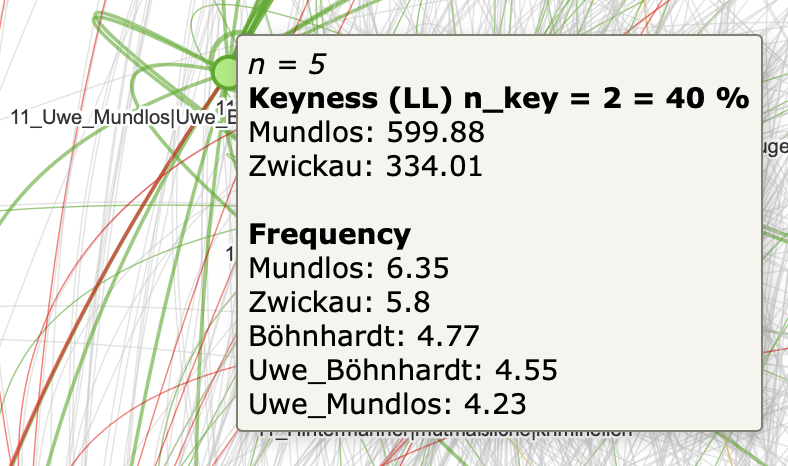
\includegraphics[width=\textwidth]{figures/media/image21.png}
  \caption{\label{fig:cluster-tooltip-nsu-mundlos}Tooltip zum Cluster \cluster{11\_Uwe\_Mundlos{\breakbar}Uwe\_Böhnhardt{\breakbar}Böhnhardt.}}
\end{figure}

Entscheidend bei der Interpretation des Graphen ist es, die enthaltenen Cluster als FE bzw. Slots eines Extremismus-Frames zu lesen und die in ihnen gebündelten Wörter als mögliche Filler des Slots bzw. zugleich Frame-evozierende LE. So kann das in \figref{fig:cluster-tooltip-nsu-mundlos} gezeigte Cluster als Teil eines größeren NSU-Frames interpretiert werden, in dem insbesondere die Mitglieder Uwe Böhnhardt und Uwe Mundlos, aber auch Zwickau als Wohnort des NSU enthalten sind. Ausdrücke wie \emph{Mundlos}, \emph{Zwickau} und \emph{Böhnhardt} wären dann dieses FE evozierende LE und zugleich die frequentesten Filler des Slots auf Token-Frame-Ebene. Aufgrund der Rekursivität von Frames können auch FE selbst als Frames gelesen werden. Durch die Einbettung in den Extremismus-Frame sind sie dabei zugleich in Hinblick auf dieses Thema perspektiviert (siehe \chapref{kollokation-von-word-embedding-clustern-als-frame-relationen-und-perspektivierung-kollokationsnetzwerke-als-frames}). Richtlinie bei der Interpretation der WE-Cluster als FE ist es, den größten gemeinsamen semantischen Nenner der enthaltenen Wörter zu identifizieren. \tabref{tab:example_clusters} in \chapref{geclusterte-word-embeddings-als-frame-elemente} zeigte bereits eine Auswahl von Clustern, die recht unkompliziert interpretierbar sind. Häufig sind Cluster jedoch, gerade wenn sie mehr Wörter umfassen, semantisch vager oder nur unter Ausblendung einzelner ‚Ausreißer` auf einen konzisen semantischen Nenner zu bringen. Dies betrifft etwa auch das zuvor genannte Cluster \cluster{11\_Uwe\_Mundlos{\breakbar}Uwe\_Böhnhardt{\breakbar}Böhnhardt}, das neben einem Teil der Mitglieder auch einen der Wohnorte des NSU enthielt oder mehr noch das Cluster \cluster{11\_Terrorzelle{\breakbar}Zwickauer\_Zelle{\breakbar}Zwickauer\_Terrorzelle}, das mit insgesamt 27 Wörtern größer ist und den NSU einerseits explizit in Hinblick auf Terror (u.\,a. \emph{Terrorzelle}, \emph{Rechtsterroristen}, \emph{Zwickauer\_Terrorzelle}) und Rechtsextremismus (u.\,a. \emph{rechten\_Szene}, \emph{rechtsextremen}) framet; andererseits aber auch Unterstützer des NSU wie \emph{Holger\_G} und \emph{Carsten\_S} enthält. Es findet sich dabei auch ein Mörder, der -- abgesehen von der durch die Handlung begründeten paradigmatischen Ähnlichkeit -- in keinem Zusammenhang zum NSU steht (\emph{Thomas\_S}). Das FE ist also insgesamt etwas vager als das zuvor betrachtete Cluster. Daran zeigt sich auch, dass nicht zu erwarten ist, etwa alle Akteure eines NSU-Frames im selben Cluster zu finden. Dies liegt darin begründet, dass sie jeweils in unterschiedliche Syntagmen eingebettet und mithin unterschiedlich geframet werden. Anschaulich macht das auch das wiederum separate Cluster \cluster{11\_Beate\_Zschäpe{\breakbar}Zschäpe{\breakbar}Nsu}, das neben diesen drei Ausdrücken auch das Wort \emph{Bundesanwaltschaft} enthält. Dieses FE ist deutlich stärker in den Bereich des juristischen Vokabulars eingebunden, da über Beate Zschäpe ausführlich als Hauptangeklagte im NSU-Prozess berichtet wurde. Am Beispiel des Clusters \cluster{08\_Intoleranz{\breakbar}Homophobie{\breakbar}Fremdenfeindlichkeit} wiederum zeigt sich, dass es wichtig ist, auch über das Cluster-Label hinaus Wörter bei der Interpretation einzubeziehen. So enthält das Cluster neben weiteren diskriminierungsbezogenen Wörtern (\emph{Diskriminierung}, \emph{Ausgrenzung}), auch Ausdrücke wie \emph{Gentrifizierung}, \emph{Hetze} oder \emph{Aggression}, die also auch andere negativ bewertete gesellschaftliche Handlungen bzw. Prozesse, die mehr oder weniger gegen Menschen gerichtet sind, umfassen.

Aufgrund der sehr hohen Knotenanzahl von 450--1413 Clustern pro Teilkorpus wäre eine Annotation der Cluster nur bei sehr umfangreichen Projekt-Ressourcen möglich. Wesentlich realistischer -- und so auch hier praktiziert -- ist es, die Interpretation der Cluster \emph{ad-hoc} vorzunehmen und einzelne Cluster nur dann im Detail zu untersuchen, wenn sie wesentlicher Bestandteil der Analyse werden. Als Beispiel mag der Hanau-Frame dienen (siehe \figref{fig:hanau-frame-2020-21} in \chapref{kollokation-von-word-embedding-clustern-als-frame-relationen-und-perspektivierung-kollokationsnetzwerke-als-frames}). Für eine erste Interpretation genügt es hier, sich einen Überblick über die angeschlossenen FE zu verschaffen. Es lässt sich, ohne die genauere Zusammensetzung der einzelnen Cluster wie \cluster{20\_tötete{\breakbar}tötet{\breakbar}erschoss}, \cluster{20\_Schmerz{\breakbar}Trauer{\breakbar}Scham} oder \cluster{20\_Gedenkfeier{\breakbar}Gedenkveranstaltung{\breakbar}Trauerfeier} zu betrachten, bereits mit großer Wahrscheinlichkeit sagen, dass es bei ersterem um die extremistische Gewalthandlung des Anschlags geht; bei zweiterem um emotionale Reaktionen auf den Anschlag sowie bei letzterem um Reaktionen in Form eines Gedenken an die Opfer des Anschlags. Diese wahrscheinlichen Vermutungen können zudem über einen Blick auf die an die jeweiligen FE angeschlossenen Cluster sowie die in den Tooltips ersichtlichen weiteren enthaltenen Wörter abgesichert werden. Dass dies funktioniert, liegt an der Kontextualisierungsleistung von Syntagmen und Paradigmen, die in der Methode aufgeht. Sollten auf diese Weise nur schwer interpretierbare Verbindung für die weitere Analyse relevant erscheinen, müsste die Verbindung der beiden Cluster näher geprüft werden: Welche der enthaltenen Wörter kookkurrieren hier tatsächlich (dies ist quantitativ überprüfbar) und worin besteht die Frame-Relation zwischen beiden Clustern (hier kann bei überschaubaren Frequenzen etwa eine Konkordanzsuche einen guten Überblick geben).

Während die Interpretation eines Knoten als FE einfach ist, wenn das Cluster sehr klein ist und womöglich nur ein Wort enthält -- in diesem Falle ist es in aller Regel sinnvoll, das Wort als FE bzw. Frame-Namen aufzufassen, etwa \cluster{20\_Hanau} und seine angeschlossenen FE als Hanau-Frame zu begreifen --, sind auch sehr große Cluster mit zum Teil über 8000 Wörtern im Graphen enthalten (z.\,B. \cluster{sp\_Gurgeltests{\breakbar}Zustellungen{\breakbar}Familienzusammenführungen}). Diese sind kaum sinnvoll interpretierbar und enthalten fast ausschließlich niedrigfrequente Wörter. Da diese FE häufig nicht im Sinne ihres zunächst kongruent erscheinenden Labels gedeutet werden können, sind alle Cluster mit mehr als 100 Wörtern im Graphen als Raute und alle Cluster mit über 200 Wörtern als Stern dargestellt. Weitere Möglichkeiten, mit diesen Clustern zu verfahren, werden in \chapref{methodische-limitationen-und-perspektiven} skizziert.

\subsubsection{Interpretation der Kanten}\label{interpretation-der-kanten}

Die Kanten des Graphen entsprechen aus Frame-semantischer Perspektive Frame-Relationen. Aus technisch-methodischer Perspektive sind sie zunächst \emph{Log-Likelihood}-Kollokationswerte, die zwischen den Wörtern der einzelnen WE-Cluster bestehen. Da die Darstellung aller statistisch signifikanten Kollokationsbeziehungen als Kanten zu einem hochgradig vernetzten und kaum mehr zu überblickenden Graphen geführt hätte, werden nur die jeweils 20 signifikantesten Kollokationspartner über eine Kante an einen Knoten angebunden, was zudem die Relevanz der Beziehung annäherungsweise abbildet. Genauso bedeutsam wie eine Kante zwischen zwei Knoten kann dabei auch das Ausbleiben einer solchen Verbindung sein. In dem Fall werden zwei FE, zumindest im zugrunde gelegten Kollokationsfenster, nicht in Beziehung zueinander gesetzt. Zum Beispiel werden im ungefähren Zeitraum 2002 bis 2010 FE wie \cluster{05\_Attentate{\breakbar}Attentaten{\breakbar}Bombenanschlägen} oder \cluster{08\_Gefährdung{\breakbar}Bedrohung{\breakbar}Störung} nicht in Verbindung zu Clustern des Rechtsextremismus gesetzt. Inwiefern in dieser Zeit, in der keine größeren (als solche erkannten) rechtsextremen Anschläge stattgefunden haben, entsprechende FE noch als Teil des gesellschaftlichen Wissens zu Rechtsextremismus gelten können, ist auf Basis der Daten nicht ohne Weiteres zu entscheiden. Ob also von einer Nullinstantiierung bzw. einem Default-Wert auszugehen ist, bei der die Frame-Relation so sehr im verstehensrelevanten Wissen verankert ist, dass sie nicht mehr verbalisiert wird, ist bei Fällen, wo das Ausbleiben einer solchen Beziehung überrascht, im Einzelfall nachzuprüfen und hermeneutisch zu entscheiden. Im genannten Fall erscheint dies jedoch eher unplausibel, da mit Aufdeckung des NSU im Jahr 2011 entsprechende Framing-Muster in aller Deutlichkeit zurückkehren und mithin wohl kein selbstverständlicher Teil des verstehensrelevanten Wissens mehr waren.

Auch die Interpretation der Kanten als Frame-Relationen muss in der Regel \emph{ad-hoc} und auf der Basis von Vorwissen erfolgen. Dies ist im Falle eines Clusters wie \cluster{we\_Kampf\_gegen} und den angeschlossenen Kanten in weiten Teilen gut möglich. Die angeschlossenen Frame-Elemente \cluster{we\_Missbrauch}, \cluster{we\_Armut}, \cluster{we\_Virus}, \cluster{we\_Terrorismus{\breakbar}Terror} sind häufige Objekte der Bekämpfung, Frame-Elemente wie \cluster{we\_Strategie}, \cluster{we\_Anstrengungen} oder \cluster{we\_Bemühungen} spezifizieren, wie und dass ein Kampf gegen etwas geführt wird. Nicht gleichermaßen eindeutig verhält es sich im Falle angeschlossener Akteure wie \cluster{we\_Extremisten{\breakbar}Dschihadisten{\breakbar}Terroristen} oder \cluster{we\_Terrormiliz{\breakbar}Al-kaida{\breakbar}Kabul}, die ja gleichermaßen Objekt der Bekämpfung als auch das den Kampf gegen etwas führende Subjekt sein können.

\largerpage
Zwei weitere potenziell bedeutungstragende Elemente sind im Graphen angelegt, da sie Informationen für die algorithmische Berechnung der Graph-Struktur bieten. Sie sind jedoch bei den hohen hier verwendeten Knotenanzahlen kaum in der Visualisierung erkennbar und werden auch in der Analyse keine weitere Berücksichtigung finden. Dies betrifft zum einen die Gerichtetheit der Kanten, die auf den ihrerseits gerichteten Kollokationen beruhen. Zwar kann es bedeutend sein, wenn sich ein Cluster unter den 20 signifikantesten Kollokatoren eines anderen Clusters findet, die Kollokation in die andere Richtung jedoch nicht gleichermaßen signifikant ist; aus Gründen der Komplexitätsreduktion kann dies jedoch in der Analyse nicht weiter berücksichtigt werden. Visuell ist diese Information zwar im Graphen enthalten, gleichwohl aufgrund ihrer geringen Bedeutung für die Analyse nur dezent markiert. So verlaufen im Fall einer beidseitig gerichteten Kollokation zwei Kanten zwischen den beiden Knoten, was aber nur bei starkem Zoom ersichtlich ist. Das zweite bei der Berechnung zugrunde gelegte, jedoch nicht sehr deutlich hervortretende Element ist die auf dem \emph{Log-Likelihood}-Wert beruhende Stärke der Verbindung zwischen zwei Knoten, die durch die Breite der Kante angezeigt wird. Hier sind nur die über alle Werte gesehen besonders signifikanten Verbindungen durch breitere Kanten gut sichtbar, häufig im thematischen Bereich Politik (z.\,B. die Kanten um das Cluster \cluster{we\_Cdu{\breakbar}Union}). Inwiefern andere Knoten eher starke oder eher schwache Verbindungen aufweisen, ist jedoch kaum zu erkennen. Dieses Problem wird dadurch gemindert, dass z.\,B. im Teilkorpus 2002--2004 mit einem mittleren \emph{Log-Likelihood}-Wert von 558,17 (arithmetisches Mittel) bzw. 194,93 (Median) und einem Minimum von 8,33 ohnehin alle dargestellten Kollokationen äußerst stark sind.

\subsubsection{Interpretation der räumlichen Struktur}\label{interpretation-der-raeumlichen-struktur}

Neben den Knoten und Kanten ist auch die räumliche Struktur des Graphen bedeutungstragendes Element der Visualisierung und soll im Folgenden beschrieben werden.

Insgesamt weisen die Netzwerke eine annähernd runde Struktur auf, die durch mindestens vier, mitunter auch einzelne weitere, Cluster bzw. Communities geprägt ist. Die Bildung der Communities beruht auf einer besonders hohen Vernetzung unter den jeweils enthaltenen Knoten, denn Knoten sind umso näher beieinander positioniert, je ähnlicher ihre Verbindungen sind. Hier schlägt sich also erneut eine paradigmatische distributionelle Ähnlichkeit nieder, sodass semantisch ähnliche Knoten häufig in der Nähe voneinander zu finden sind und sich auch innerhalb der Netzwerk-Cluster kleinere thematische Cluster bilden, so z.\,B. in der Community ‚Straftaten \& Juristisches` eine Gruppe mit Knoten wie \cluster{ta\_Gefängnis}, \cluster{ta\_Knast} und \cluster{ta\_Festnahmen{\breakbar}Verhaftungen}, eine andere mit Knoten wie \cluster{ta\_Ermittler}, \cluster{ta\_Ermittlern} und \cluster{ta\_Verdacht} sowie eine weitere mit Clustern wie \cluster{ta\_Klägerin{\breakbar}Kläger{\breakbar}Richterin}, \cluster{ta\_Berufung{\breakbar}Revision} oder \cluster{ta\_Richter{\breakbar}Staatsanwalt}. Auch die Positionierung einzelner Knoten im Verhältnis zu den Communities kann gemäß dem probabilistischen Charakter der Methode fruchtbar gedeutet werden. Zwar ist jeder Knoten zunächst durch den Algorithmus nur einer der Communities zugeordnet, jedoch graduell auch mit anderen Communities mehr oder weniger vernetzt, was sich durch die räumliche Nähe zu ebendiesen ausdrückt. Besonders sichtbar wird dies an den Knoten, die am Übergang von zwei Communities positioniert sind. Diese lassen sich i.d.R. auch semantisch beiden Communities zuordnen, so z.\,B. die Cluster \cluster{14\_Antrag} und \cluster{14\_Ausschuss{\breakbar}Untersuchungsausschuss{\breakbar}NSA-Untersuchungsausschuss}, die am Übergang zwischen den Communities ‚Politik` und ‚Straftaten \& Juristisches` verortet sind oder die Cluster \cluster{08\_beteiligt\_gewesen} und \cluster{08\_getötet{\breakbar}erschossen} am Übergang der Communities ‚Krieg \& Islamismus' und ‚Straftaten \& Juristisches`.

\subsubsection{Mögliche Fallstricke bei der Interpretation}\label{moegliche-fallstricke-bei-der-interpretation}

In diesem Kapitel sollen -- mitunter bereits angedeutete -- Missverständnisse zusammengefasst werden, die bei der Interpretation der erzeugten Frames auftreten können.

Das erste mögliche Problem betrifft die analytische Fokussierung auf einzelne Datenpunkte. Die hier vorgestellte Methode bietet einen Zugang zur epistemischen Makrostruktur von Diskursen im Sinne einer Vogelperspektive auf Diskurse und des \emph{distant reading} \autocite{morettiConjecturesWorldLiterature2000}. Alle Datenpunkte (einzelne Word Embeddings, Word-Embedding-Cluster, Kollokationen zwischen den Clustern, etc.) sind zudem einem relationalen, probabilistischen Zugang entsprechend berechnet und zu deuten, d.\,h. es spielen immer Ambiguitäten und die Komplexität vieler simultaner Relationen sowie auch Zufälligkeiten eine Rolle. Letztere gehen insbesondere auf die Nicht-Determiniertheit der verwendeten Algorithmen zurück. Die Berechnung von Word-Embeddings, das Clustering ebendieser, die Visualisierung der Word-Embedding-Cluster und ihrer Kollokationswerte als Graph, und die Erkennung von Clustern im Graph nutzen Algorithmen, die -- im Gegensatz zu z.\,B. der Berechnung von Kollokationen -- Zufallskomponenten beinhalten. Zwar werden dabei im Großen und Ganzen sehr ähnliche Ergebnisse erzielt, wenn die Methoden bei identischen Parametern auf dieselben Daten angewandt werden. Einzelne Datenpunkte können jedoch durchaus unterschiedlich berechnet werden. So können etwa einzelne Word-Embeddings leicht andere nächste Nachbarn im Vektorraum haben oder in andere Cluster gezählt werden. Es wäre aus diesem Grund voreilig, Analyseschlüsse auf Detail-Ergebnissen dieser Algorithmen zu stützen. Zum Beispiel sollte daraus, dass in Cluster \cluster{20\_Susanne\_Hennig-Wellsow{\breakbar}Hennig-Wellsow{\breakbar}Mike\_Mohring} neben den thüringer Politiker*innen Susanne Hennig-Wellsow und Mike Mohring auch die Wörter \emph{Gauland}, \emph{Franziska\_Giffey} und \emph{Chrupalla} enthalten sind, noch nicht geschlossen werden, dass jede einzelne dieser Politiker*innen eine ähnliche Rolle im Extremismusdiskurs spielt und sich von benachbarten Clustern wie \cluster{20\_Schäuble{\breakbar}Bouffier{\breakbar}Dobrindt} oder \cluster{20\_Höcke{\breakbar}Kalbitz{\breakbar}Andreas\_Kalbitz} deutlich unterscheidet. Zwar zeichnet sich ab, dass das letztgenannte Cluster insbesondere AfD-Politiker und -Strukturen beinhaltet und das erstgenannte in weiten Teilen die Ereignisse um die Thüringer Ministerpräsidentenwahl 2020 widerspiegelt; warum aber z.\,B. \emph{Chrupalla} in dieses Cluster und nicht ins AfD-Cluster sortiert wurde, ist nicht auf den ersten Blick ersichtlich. Es ist außerdem wahrscheinlich, dass sich bei erneuter Berechnung der Cluster einzelne Cluster nicht erneut bilden bzw. andere Wörter umfassen. Dies bedeutet nicht, dass nicht tatsächlich Unterschiede in der Semantisierung bestehen. Sie sind sogar wertvolle Hinweise darauf, denen im Sinne einer datengeleiteten, quantitativ informierten Diskursanalyse \autocite{bubenhoferQuantitativInformierteQualitative2013} weiter nachgegangen werden kann. Sie müssten aber zunächst durch ergänzende Analysen weiter abgesichert werden (s.u.). Für die makrostrukturelle Diskursbeschreibung ist es hingegen empfehlenswert, Muster zu identifizieren, die über den einzelnen Datenpunkt hinausgehen. Dies können zum einen rekurrente Muster wie das in allen Teilkorpora bestehende Cluster um Wortformen der Lexeme \emph{antisemitisch}, \emph{rassistisch} und \emph{rechtsextrem} bzw. \emph{rechtsextremistisch} (z.\,B. \cluster{05\_rechtsextremen{\breakbar}rechtsextremistischen{\breakbar}rechtsextreme}, \cluster{14\_rechtsradikale{\breakbar}rechtsradikalen{\breakbar}Rechtsradikalen} oder \cluster{ta\_rechtsradikale{\breakbar}rechtsextreme{\breakbar}antisemitische}) sein. Dieses wiederkehrende Muster zeigt deutlich an, dass wesentliche Eigenschaften des Rechtsextremismus als solche im gesellschaftlichen Wissen verankert sind und sprachlich realisiert werden. Zum anderen ist es empfehlenswert, größere zusammenhängende Strukturen wie die als Extremismus-Varianten-Frames lesbaren Verbünde aus Knoten des Graphen zu fokussieren. Es kann auch nur so das rekontextualisierende Potenzial \autocite{bubenhoferVisuelleLinguistikZur2020} der verwendeten Methode bzw. Visualisierung erfasst und für die Analyse fruchtbar gemacht werden. Dies gilt grundsätzlich auch für die auf Kollokationen beruhenden Kanten; sie sind den angesprochenen Unsicherheiten jedoch nur in geringerem Maße unterworfen, da sie ein algorithmisch-deterministisches methodisches Element darstellen.

Ein weiterer möglicher Fallstrick, der bereits in \chapref{geclusterte-word-embeddings-als-frame-elemente} in Kürze angesprochen wurde, betrifft die Interpretation der Word-Embedding-Cluster als FE. Hier ist insbesondere zu berücksichtigen, dass Cluster weit mehr Wörter enthalten können als nur die drei Wörter, die das Label des Clusters ausmachen. So beinhaltet etwa das Cluster \cluster{99\_wirtschaftlichen{\breakbar}ökonomischen{\breakbar}ökonomische} neben den drei namensgebenden, im Vektorraum zentralsten Wörtern des Clusters und den semantisch kongruenten Wörtern \emph{wirtschaftliche} und \emph{finanziellen} auch die Ausdrücke \emph{Globalisierung}, \emph{ökologische} und \emph{ökologischen}. Während das Label des Clusters also zunächst eine Interpretation als rein wirtschaftsbezogenes FE nahelegt, sind auch Aspekte der Ökologie und Globalisierung im Cluster enthalten. Letztlich beruht jedoch die Nachbarschaft im Vektorraum und mithin die Zuordnung zu einem gemeinsamen Cluster auf dem musterhaften Auftreten in ähnlichen Kontexten und es ist durchaus sinnvoll, das Wort \emph{Globalisierung} als stark assoziiert mit ökonomischen und ökologischen Fragen zu sehen. Insofern ist es an dieser Stelle empfehlenwert, das Cluster zunächst als eher vages Frame-Element zu lesen, das insgesamt den Bereich von Ökologie, Ökonomie und Globalisierung betrifft. Wann immer die genaue Beziehung des FE zu anderen FE von Interesse ist, müssten genauere Analysen erfolgen, welche Wörter der beiden Cluster tatsächlich kookkurrieren.

Hiermit ist zugleich ein weiterer möglicher Fehlschluss angesprochen, der bei der Interpretation des Graphen gemacht werden kann und die Kanten bzw. Frame-Relationen betrifft. So beruhen die eingezeichneten Kanten ja auf Kollokationen der Wörter des einen Clusters mit Wörtern des anderen Clusters, wobei die einzelnen Wörter und ihr individuelles Kollokationsverhalten nicht mehr berücksichtigt werden. Hierdurch wirken sich frequentere Wörter auch stärker auf die Kollokationen des Clusters aus als weniger frequente Wörter. Einzelne Verbindungen können also eher durch einzelne Wörter geprägt sein sowie insgesamt eher durch die frequenteren Wörter des Clusters.\footnote{Insgesamt liegt den Word-Embedding-Clustern jedoch eine paradigmatische Ähnlichkeit zugrunde, sodass grundsätzlich von einem ähnlichen Kollokationsverhalten der Wörter auszugehen ist (siehe \chapref{was-sind-word-embeddings}).} Des Weiteren ist bei der Interpretation der Kanten zu beachten, dass nur die 20 signifikantesten Kollokationen eines jeden WE-Clusters an es angebunden sind (siehe auch \chapref{berechnung-des-extremismus-centroid-und-begrenzung-der-knotenmenge}). Besteht also zwischen zwei Knoten keine Kante, bedeutet dies nicht, dass nicht auch diese Cluster signifikant kookkurrieren. Sie sind nur jeweils nicht unter den Top-Kollokatoren des anderen Clusters vertreten. Die genauen Kollokationsdaten sind bei Bedarf über die Korpussoftware abrufbar.

\largerpage
Letztlich ist noch einmal auf einen Nachteil der auf \emph{Word2Vec} und ähnlichen Algorithmen basierenden Word Embeddings hinzuweisen. Wie in \chapref{was-sind-word-embeddings} dargestellt, handelt es sich bei ihnen um Type-basierte Algorithmen, die also für jeden Korpus-Type im Sinne eines formseitig identischen Tokens eine Vektorrepräsentation berechnen. Bei der Berechnung werden alle Belegstellen für diese Types herangezogen, was bei homonym bzw. polysem oder metonymisch gebrauchten Wörtern ein Problem darstellen kann. Sind etwa Wörter wie \emph{Björn\_Höcke}, \emph{Andreas\_Kalbitz} und \emph{Flügel} im Cluster \cluster{20\_Höcke{\breakbar}Kalbitz{\breakbar}Andreas\_Kalbitz} zusammengefasst, beruht das darauf, dass \emph{Flügel} als Name einer Parteistruktur gebraucht wird und daher nicht etwa mit Wörtern wie \emph{Schwingen}, \emph{Schnabel} oder \emph{Federn} zusammengefasst ist, die das Wort noch im Zeitraum 2011--2013 im Vektorraum umgeben. Interessant -- aber auch komplexitätssteigernd -- wäre es, unterschiedliche Embeddings für die Bedeutungen zu haben, was im Rahmen der hier verwendeten Algorithmen jedoch nicht ohne Weiteres zu realisieren ist. Grundsätzlich wäre auch denkbar, dass homonyme Wörter bei sehr unterschiedlichen Verwendungskontexten gar keine sinnvolle Vektorrepräsentation erhalten und somit für die Analyse nicht nutzbar sind. Dass Wörter im Korpus gleichermaßen in unterschiedlichen Bedeutungen vorkommen, ist jedoch aufgrund der korpuspragmatischen Kontextualisierung eher unwahrscheinlich. So kommt das Wort \emph{Bank} in Zeitungstexten in aller Regel in seiner Bedeutung als Finanzinstitut, nicht als Sitzgelegenheit vor. Folglich sind seine nächsten Nachbarn im Vektorraum des Zeitraums 2020--2021 \emph{Sparkasse}, \emph{Commerzbank} und \emph{Greensill}.\footnote{Ein Beispiel für ein durch Polysemie geprägtes paradigmatisches Profil ist das Umfeld des Wortes \emph{Flügel} im Word-Embedding-Modell 2014--2016. Unter den 10 nächsten Nachbarn finden sich sowohl \emph{rechten\_Flügel}, \emph{linken\_Flügel} und \emph{Parteiflügel}, die auf einen eher politischen Gebrauch hindeuten; \emph{Saiten}, was auf das Musikinstrument deutet sowie \emph{Propeller}, was den Gebrauch des Wortes \emph{Flügel} in der Luftfahrt widerspiegelt.} Neben der übergreifenden Disambiguierung durch den medialen Kontext bietet auch die diachrone Unterteilung des Korpus dieses Potenzial. So können die Wörter, die nicht konstant mehrdeutig gebraucht werden, durch das Kriterium der thematischen Einschlägigkeit in die Frame-Modellierung ein- oder ausgeschlossen werden. Wörter wie \emph{Hanau}, \emph{Querdenker} oder \emph{Lkw} sind dann nur in den Jahren, in denen sie für die Modellierung eines Extremismus-Frames relevant sind, in der Darstellung enthalten. Auch da die jeweils angeschlossenen Kanten ebenfalls thematisch in Hinblick auf Extremismus perspektiviert sind, wird nicht unnötigerweise das gesamte Bedeutungsspektrum eines Ausdrucks im Frame aufgefächert.
